
%%%%%%%%%%%%%%%%%%%%%%%%%%%%%%%%%%%%%%% Chapter 5

\chapter{Topology of the Complex Plane and Continuity}



\section{Point-set topology in the (extended) complex plane}


The complex plane has the same topology as the Euclidean plane $\mathbb{R}^2$.  As a result, the convergence concepts and limits in the real case and the complex case are basically the same. The concepts of point-set topology in $\mathbb{R}^2$ can be directly imported to the complex case.
For example, open disc is defined as follows.
\begin{svgraybox}
	\begin{definition} \index{Open disk}
		The \df{open disk} of radius $r$ centered at $z_0$ is the set
		$$
		D(z_0,r) \triangleq \{z\in\mathbb{C}:\, |z-z_0|<r\}.
		$$
	\end{definition}
\end{svgraybox}

The collection of all open disks $D(z,r)$, with $z$ varying over all points in $\mathcal{C}$, and $r>0$, is the base of the standard topology on $\mathbb{C}$.

\begin{svgraybox}
	\begin{definition} \index{Open set} \label{def:open_set}
		A subset $A$ in $\mathbb{C}$  is called an \df{open set} for every point $z_0\in A$, we can find a sufficiently small radius $r$ so that $D(z_0,r)$ is a subset of $A$. A set $B$ is said to be \df{closed} if the complement of $B$ in $\mathbb{C}$ is open, i.e., for any point $w_0$ that is not in $B$, there is radius $r$ such that $D(w_0,r)$ and $B$ are mutually disjoint.
	\end{definition}
\end{svgraybox}

\begin{example}
	The upper half-plane $\imag(z) >0$ is open. Given any point $z$ in the upper half-plane, we can enclose it by an open disk $D(z, |z|/2)$, which lies inside the upper half-plane. 
\end{example}

\begin{example}
	The set $D(z_0,r)$ is open according to Definition~\ref{def:open_set}. Pick any point $w\in D(z_0,r)$. The distance between $w$ and the closest point on the circle $|z-z_0|=r$ is  $r - |w-z_0|$. The set $D(w, (r-|w-z_0|)/2)$ lies inside the set $D(z_0,r)$, hence $D(z_0,r)$ is an open set.
\end{example}

\index{Topological space}
It is not difficult to show that (i) the empty set is open, (ii) the whole complex plane is open, (iii) arbitrary union of open sets is open, and (iv) intersection of finitely many open sets is open. These are the axioms of open sets in topology. In general, given a set $X$ and a collection $\mathcal{T}$ of subsets of $X$ that satisfies these four axioms, the pair $(X,\mathcal{T})$ is called a \df{topology space}. 

\smallskip

In the extended complex plane, we also need a notion of open disks centered at the point at infinity. A convenient way to formalize this is to use the inversion map  $w =f(z)=1/z$. Under this transformation, a small disk around the origin in the $w$-plane,
$$\{w\in\mathbb{C}:\, |w|<\epsilon\},$$
corresponding to a neighborhood of $\infty$ in the $z$-plane. Thus an open disk centered at infinity is any set of the form
$$\{ \, z\in \mathbb{C}:|z|>R\, \} \cup \{ \infty \} ,$$
for some radius $R>0$. Geometrically speaking, a point with very large modulus is close to the point at infinity.



\begin{remark} \index{Neighborhood of a point}
	In this book, the term ``\df{neighborhood of a point}'' will mean a set $S$ whose interior contains the given point. In other words, a set $S$ is a neighborhood of point $p$ if we can find a small disc centered at $p$ that is completely inside $S$. A neighborhood of a point needs not be an open set. We will use the term ``open neighborhood'' to refer to a neighborhood that is an open set. 
\end{remark}


The concept of accumulation point, closure, interior, and isolated point are defined in the same way as in Euclidean plane. We briefly review them in the remainder of this section.

\begin{svgraybox}
	\begin{definition} \index{Closed set} \index{Accumulation point}
A set $S$ is called $\df{closed}$ if its complement $S^c = \mathbb{C}\setminus S$ is open. A point $z$ in $\mathbb{C}$ is called an \df{accumulation point} of a set $A$ if, for all $r>0$, we can find a point $z\in D(z_0,r)\cap A$ that is different from~$z_0$.
	\end{definition}
\end{svgraybox}

We can prove that a set $A$ is closed if and only if $A$ contains all of its accumulation points. 

\begin{svgraybox}
	\begin{definition}
We define the \df{closure} of a set $S$ as the union of $S$ and the accumulation points of~$S$, and use the notation $\overline{S}$ to refer to the closure of $S$.
	\end{definition}
\end{svgraybox}

%Notation: we will denote the closure of a set $S$ by $\overline{S}$.


\begin{example} the closure of open disk $D(z_0,r)$ is the set of complex numbers $z$ that satisfy the inequality $|z-z_0|\leq r$. We will denote a closed disk centered at $z_0$ with radius $r$ by $\overline{D}(z_0,r)$. 
\end{example} 


\begin{example}
Given two real numbers $a$ and $b$ with $a<b$, the annulus $\{z: a\leq |z| \leq b\}$ is a closed set. The accumulation points lie on the circle $|z|=a$ and $|z|=b$.
\end{example}

\index{Discrete set} \index{Isolated point}
\begin{svgraybox}
	\begin{definition} \label{def:discrete_set} 
Given a set $S\subseteq \mathbb{C}$, a point $z\in S$ is called an \df{isolated point} of $S$ if we can find a radius $r>0$ such that $D(z,r)\cap S = \{z\}$. A set $S$ is said to be \df{discrete} all points in $S$ are isolated.
	\end{definition}
\end{svgraybox}


Geometrically, the points in a discrete set are separated from each other by some positive distance. It can be shown that a discrete set is closed, but do not have any accumulation point.

\begin{example}
	The set of points 
	$\{1/n: n\in \mathbb{N}_{>0}\}$ is discrete. However, the set of points
	$\{1/n: n\in \mathbb{N}_{> 0}\} \cap \{0\}$ is not discrete, because the origin is an accumulation point.
\end{example}

%\begin{example}
%	This example illustrates the distinction between being \emph{non-isolated in the ambient
%	space} and being an \emph{accumulation point of the set}. Consider the subset
%	\[
%	S = \left\{ \frac{1}{n} : n \in \mathbb{N} \right\} \subseteq \mathbb{C}.
%	\]
%	
%	First observe that no point of $\mathbb{C}$ is isolated in the ambient topology: for any
%	$z \in \mathbb{C}$ and any $r>0$, the disk $D(z,r)$ contains infinitely many complex
%	numbers distinct from $z$. Thus every point of $\mathbb{C}$ is ``non-isolated'' in the
%	ambient space.
%	
%	Now consider the point $z=2$. Since $2 \notin S$, it cannot be an isolated point of $S$.
%	However, $2$ is also \emph{not} an accumulation point of $S$. Indeed, taking $r=1$ gives $D(2,1) \cap S = \emptyset$,
%	so there exists a neighborhood of $2$ that contains no points of $S$ at all. Hence $2$ is
%	neither an isolated point of $S$ nor an accumulation point of $S$, even though it is not
%	isolated in the ambient space $\mathbb{C}$.
%
%	
%	This example shows that the property of being ``non-isolated in the ambient space'' has no
%	direct bearing on whether a point is an accumulation point of a given subset.
%\end{example}



\begin{example} (Point lattice in complex plane)
Let $w_1$ and $w_2$ be two nonzero complex numbers that are linear independent as vectors. The set of points
$$
\{aw_1 + bw_2: a,b\in \mathbb{Z}\}
$$
is a discrete set.
\end{example}





\section{Limit and continuity of complex function}



\begin{svgraybox}
	\begin{definition} (Limit of function)  
		\index{Limit of complex function} Let $f$ be a complex function defined on a set $S \subseteq \mathbb{C}$, and let $z_0$ be a point in the closure of $S$. We say that $f(z)$ \df{converges} to a complex number $w$ as $z\rightarrow z_0$ if  for each $\epsilon>0$, we can find $\delta>0$ such that for all
		$
		z\in S$ satisfying  $0<|z-z_0|< \delta$, we have $|f(z)-w| <\epsilon$.
	\end{definition}
\end{svgraybox}

We note that the value of $f$ at $z_0$ is irrelevant in the above definition. In the case when $z_0$ is an accumulation point of $S$ but not in $S$, then the function value $f(z_0)$ is undefined. However, if the limit exists, the value of the limit is determined uniquely by the value of function $f(z)$ for $z$ close $z_0$ (Exercise~\ref{exercise:unique_limit}).

If we take the point at infinity into account, we define the limit of a function  as follows:

\begin{enumerate}
	\item When $z_0$ is finite and the limit $w$ is $\infty$, $\lim_{z\rightarrow z_0} f(z) =\infty$ means 
	$$
	\lim_{z\rightarrow z_0} \frac{1}{f(z)} = 0. 
	$$
	\item When $z_0=\infty$  and $w$ is finite, $\lim_{z\rightarrow \infty} f(z) = w$ means 
	$$
	\lim_{z\rightarrow 0} f(1/z) = w. 
	$$
	\item When both $z_0$  and  $w$ is $\infty$, $\lim_{z\rightarrow \infty} f(z) =\infty$ means 
	$$
	\lim_{z\rightarrow 0} \frac{1}{f(1/z)} = 0. 
	$$
\end{enumerate}





\begin{svgraybox}
	\begin{definition} \index{Continuous!function} (Function continuity)
		A function $f:S \rightarrow\mathbb{C}$ defined on a set $S\subseteq \mathbb{C}$ is said to be \df{continuous at a point} $z_0 \in S$ if, for any $\epsilon>0$, there exists $\delta>0$ such that
		$$
		(z\in S \text{ and } |z - z_0| <\delta )\ \Rightarrow\ |f(z)-f(z_0)| < \epsilon.
		$$
		A function $f$ is said to be \df{continuous} in a domain $S$ if $f$ is continuous at every point in~$S$. \label{def:continuous_function}
	\end{definition}
\end{svgraybox}

The definition of continuity at a point is the same as requiring that (i) $f(z_0)$ exists, (ii) $\lim_{z\rightarrow z_0} f(z)$ exists, and (iii) $\lim_{z\rightarrow z_0} f(z) = f(z_0)$.

We note that by the definition of continuity at a point, a function is always continuous at an isolated point.

Continuity at the point at infinity is defined by: given a function $f:S\rightarrow\mathbb{C}$, we say that $f$ is continuous at the point at infinity if
for all  $\epsilon>0$, there exists $R>0$ such that
$$
(z\in S \text{ and } |z | >R )\ \Rightarrow\ |f(z)-f(\infty)| < \epsilon.
$$



In the next theorem, the value of $w_0$, $z_0$ nad $\zeta$ may be the point at infinity. This is a result on the Riemann sphere.

\begin{svgraybox}
	\begin{theorem} (Limit of composite function)
		Let $f(z)$ and $g(w)$ denote complex functions Suppose $f(z)$ converges to $w_0$ as $z\rightarrow z_0$, $g(w)$ converges to $\zeta$ as $w\rightarrow w_0$, and $g$ is continuous at $w_0$. Then, 
		$$
		\lim_{z\rightarrow z_0} g(f(z)) = \zeta.
		$$
	\end{theorem}
\end{svgraybox}

If the point at infinity is allowed in the domain of $f$ and $g$, then the proof of the above theorem requires the consideration of several cases, depending on whether $z_0$, $w_0$ and $\zeta$ are finite or $\infty$.

By consider the real and imaginary part separately, we can prove the following

\begin{svgraybox}
	\begin{theorem}
		A complex function $f$ is continuous if and only if the real and imaginary parts are continuous.
	\end{theorem}
\end{svgraybox}

The proof of this theorem is straightforward and is omitted.

Another way to understand continuity is by means of sequence. If a complex function $f$ is continuous at $z_0$, and if $(z_k)_{k=1}^\infty$ is a sequence of complex numbers converging to $z_0$, then the image points $(f(z_k))_{k=1}^\infty$ should converge to $f(z_0)$. We can approach $z_0$ from any direction, and the limit of the sequence should equal $f(z_0)$.




The limit for complex function behaves in the same as the limit of vector function. Hence, complex limit has the same properties as in multi-variable calculus.  







\begin{example} Show that $f(z) = 1/z$ is continuous in the domain $\mathbb{C}\setminus\{0\}$.
	
	Suppose $z=x+iy$ and $z\neq 0$.
	\[
	\frac{1}{z} = \frac{1}{x+iy} 
	= \frac{x-iy}{x^2+y^2} 
	\]
	The real part of $f(z)$ is $x/(x^2+y^2)$ and the imaginary part is $-y/(x^2+y^2)$. Both of them are continuous functions in the domain $\mathbb{C}\setminus\{0\}$. Hence $f(z)$ is continuous by the previous theorem.
\end{example}


\begin{example}
	We compute the limit of the linear fractional transformation $f(z) = \frac{z+i}{z-8}$ as $z$ approaches $\infty$.  We first write the function as
	$$
	\frac{z+i}{z-8} = 
	\frac{z-8+8+i}{z-8}= 1 + \frac{8+i}{z-8}.
	$$
	Since we are considering $z\rightarrow \infty$, the fractional $(8+i)/(z-i)$ will tend to 0, and the limit is~1.
	
	If we want to verify that the answer is indeed equal to 1 by definition, we need to bound
	$$
	\Big| \frac{z+i}{z-8} -  1\Big| =
	\Big| \frac{8+i}{z-8}\Big| = \frac{\sqrt{65}}{|z-8|}.
	$$
	Using the reverse triangular inequality, we know that $|z-8| \geq |z|-8$. Let $\epsilon$ be a positive real number. If we set 
	$$
	r = \frac{\sqrt{65}}{\epsilon}+8,
	$$
	then for all $z$ with modulus $|z|>r$, we have
	$$
	\frac{\sqrt{65}}{|z-8|} \leq
	\frac{\sqrt{65}}{|z|-8} \leq
	\frac{\sqrt{65}}{r-8} = \epsilon.
	$$
	This proves that
	$$
	\lim_{z\rightarrow \infty} \frac{z+i}{z-8} = 1.
	$$
\end{example}



Another way to understand continuity is by means of sequence. If a complex function $f$ is continuous at $z_0$, and if $(z_k)_{k=1}^\infty$ is a sequence of complex numbers converging to $z_0$, then the image points $(f(z_k))_{k=1}^\infty$ should converge to $f(z_0)$. We can approach $z_0$ from any direction, and the limit of the sequence should equal $f(z_0)$.



The limit for complex function behaves in the same as the limit of vector function. Hence, complex limit has the same properties as in multi-variable calculus.  


The next theorem is an expected result, because the analogous result holds for real functions.

\begin{svgraybox}
	\begin{theorem}
		The composition of two continuous complex functions is continuous.
	\end{theorem}
\end{svgraybox}


Let $f(z)$ be a complex-valued function mapping from a set $A \subseteq \mathbb(C)$ to $\mathbb{C}$.
We define the pre-image of a set $S\subseteq \mathbb{C}$ under a function $f(z)$ by
$$
f^{-1}(S) \triangleq \{z \in A:\, f(z) \in S\}.
$$
Using this notation, we can characterize continuity as:

\begin{svgraybox}
	\begin{theorem} \label{thm:continuous_preimage}
A complex function $f: A \rightarrow \mathbb{C}$ is continuous if and only if for all open set $U \subseteq \mathbb{C}$, the pre-image $f^{-1}(U)$ is an open set in~$A$. 
	\end{theorem}
\end{svgraybox}

Proof is left as an exercise (Exercise~\ref{exercise:continuous_preimage}).


\section{Paths and parametric curves}


\index{Parametric curve} \index{Path} 
\begin{svgraybox}
	\begin{definition}
A \df{path}/\df{parametric curve} is defined as a continuous function $\gamma$, that maps a closed interval $[a,b]$ to the complex numbers $\mathbb{C}$:
		\begin{equation}
			\gamma :\, [a,b] \rightarrow \mathbb{C}.
			\label{eq:parametric_curve_def}
		\end{equation}
The \df{trajectory} or \df{locus} of a path is the set of points that is equal to the image of a path $\gamma: [a,b]\rightarrow\mathbb{C}$. We  denote the trajectory of $\gamma$ by $|\gamma|$.
	\end{definition}
\end{svgraybox} 
We call $\gamma(a)$ and $\gamma(b)$ the initial point and end point, respectively. We say that the curve represented by $\gamma$ goes from $\gamma(a)$ to $\gamma(b)$. Since $\gamma$ is continuous, the locus of a parametric curve is a compact set.

\index{Line segment}
Given two distinct complex numbers $z_1$ and $z_2$, the line segment from $z_1$ to $z_2$ can be represented parametrically by
$$
\gamma(t) = z_1(1-t) + z_2 t
$$
for $t\in [0,1]$. Alternately, we may represent the same trajectory by
$$
\tilde{\gamma}(t) = z_1(1-t^2) + z^2 t^2
$$
for $t\in [0,1]$. How a curve is parameterized is part of the data of parametric curve. As a result, $\gamma(t)$ and $\tilde{\gamma}(t)$ are considered two different parametric curve, even though the underlying trajectory is the same. We will call a path a {\em line segment} from $z_1$ to $z_2$ if the start points and end points are $z_1$ and $z_2$, respectively, and the locus of the path consists of the points $z_1(1-t) + z_2t$, for $t\in [0,1]$.


%We will use the notation 
%\begin{equation}
%[z_1,z_2]
%\label{eq:line_segment}
%\end{equation}
%to stands for the line segment from $z_1$ to $z_2$. When $a$ and $b$ are 


A circular path centered at $z_0$ with radius $r$ and counter-clockwise orientation can be represented in polar form:
\begin{equation}
\gamma(t) = z_0 + re^{i\theta}
\label{eq:circular_path}
\end{equation}
for $\theta\in[0, 2 \pi ]$.

\index{Path!concatenation}
{\em Path concatenation.} Given two paths $\gamma_1: [a_1,b_1] \rightarrow \mathbb{C}$, and $\gamma_2: [a_2,b_2] \rightarrow \mathbb{C}$, if $\gamma_1(b)=\gamma_2(a)$, we can concatenate the two paths. The combined path 
$$\gamma: [a_1,b_1+b_2-a_2] \rightarrow \mathbb{C}$$ 
is defined as
$$
\gamma(t) \triangleq \begin{cases}
	\gamma_1(t) & \text{ for } t \in [a_1,b_1] \\
	\gamma_2(t+b_1-a_1) & \text{ for } t \in [b_1, b_1+b_2-a_2].
\end{cases} 
$$
We denote the \df{concatenated} path by $\gamma_1+\gamma_2$. Even though we use the symbol ``+'' to stand for path concatenation, it is important to note that path addition is not commutative. Moreover, if the end point of $\gamma_1$ and the start point of $\gamma_2$ do not coincide, then the sum of $\gamma_1$ and $\gamma_2$ are not defined.

However, if the concatenation of $m$ paths $\gamma_1,\ldots, \gamma_m$ is well defined, i.e., when the end point of $\gamma_i$ is the start point of $\gamma_{i+1}$, then the path summation is associative, and we will denote the overall concatenated path as
$$\gamma_1 + \gamma_2 + \cdots + \gamma_m.
$$


{\em Path negation.}
\index{Path!negation}
The \df{negation} or the \df{reverse} of a path $\gamma:[a,b]\rightarrow\mathbb{C}$ is the path with the same locus with reverse direction, denoted by $-\gamma$,
$$
(-\gamma)(t) = \gamma(a+b-t) \quad \text{for } t\in[a,b].
$$





\index{Curve!simple} \index{Curve!closed} \index{Curve!Piece-wise linear} \index{Curve!polygonal}


\renewcommand{\labelenumi}{(\alph{enumi})}
\begin{svgraybox}
	\begin{definition} The parametric curve in \eqref{eq:parametric_curve_def} is said to be
		\begin{enumerate}
			\item \df{piece-wise linear} or \df{polygonal} if it is the concatenation of finitely many line segments.
			\item \df{simple} if there is no self-intersection, i.e., $\gamma(t_1) \neq \gamma(t_2)$ for any $a\leq t_1 <t_2 \leq b$, except when $t_1=a$ and $t_2=b$.
			\item  \df{closed} if the start point is the same as the end point, i.e., $\gamma(a) = \gamma(b)$.
		\end{enumerate}
		\label{def:simple_path}
	\end{definition}
\end{svgraybox}

\begin{example}
	We can obtain very symmetrical curves using parameterization in the form
	$$
	\gamma(t) = ae^{ikt} + b e^{i\ell t}
	$$
	for $t \in [0,2\pi]$. For example, if we choose $a=5$, $b=2$, $k=3$ and $\ell=-4$, the corresponding curve is drawn in Fig.~\ref{fig:parametric_plot}. We note that this is a closed curve with  7-fold symmetry. This is a closed but not simple path.
\end{example}

\begin{figure}
	\begin{center}
		\includegraphics[width=9cm]{parametric_plot.png}
	\end{center}
	\caption{Parametric plot of $\gamma(t)=5e^{i3t} + 2e^{-i4t}$ for $0\leq t \leq 2\pi$.}
	\label{fig:parametric_plot}
\end{figure}




\section{Connected set}
\label{sec:connected_set}
\index{Separated sets}
\begin{svgraybox}
	\begin{definition}
		Two nonempty sets $A$ and $B$ in $\mathbb{C}$ are said to be \df{separated} if $\overline{A}\cap B = \emptyset$ and $A\cap \overline{B}=\emptyset$. \label{def:separated_sets}
	\end{definition}
\end{svgraybox}
In other words, $A$ and $B$ are separated set if the accumulation points of $A$ are not in $B$, and the accumulation points of $B$ are not in $A$.

\begin{example}
The two open disks $D(-1,1)$ and $D(1,1)$ are separated, even though the origin is a common accumulation point. However, the open disk $D(-1,1)$ and the closed disk $\overline{D}(1,1)$ are not separated.
\end{example}

\begin{svgraybox}
	\begin{definition}
An nonempty set $X \subseteq \mathbb{C}$ is said to be \df{disconnected} if $X$ can be written as the union of two separated sets. A set is said to be \df{connected} if it is not disconnected.
	\end{definition}
\end{svgraybox}

In other words, a connected set cannot be written as the union of two separated sets.

\begin{example}
The square lattice $\{x+iy:\, x,y\in\mathbb{Z}\}$ is disconnected. In fact, any discrete set defined in Definition~\ref{def:discrete_set} is disconnected.
\end{example}



\index{Relative topology}
We introduce a few more concepts in topology. 
Let $X$ be  nonempty subset in $\mathbb{C}$. If we regard $X$ be a metric space by itself, then the distance function pertaining to $X$ is just the restriction of the distance function of $\mathbb{C}$, namely the absolute value. However, an open set in $X$ may not be be open as a subset of $\mathbb{C}$. In view of this, an open set in $X$ will be referred to as a \df{relative open set}, a closed set in $X$ is called a \df{relative closed set}. The {\em relative topology} of $X$ is the collection 
$$
\mathcal{T}_X \triangleq \{X\cap U:\, \text{open set $U$ in $\mathbb{C}$}\}.
$$
It is straight forward to show that the sets in $\mathcal{T}_X$ satisfy the four axioms of topology, so that $(X,\mathcal{T}_X)$ is a topological space.

For example, if $X$ is the real axis in $\mathbb{C}$, the relative open sets $X$ are the same as usual open sets in $\mathbb{R}$.

\begin{example}
From real analysis, open interval $(a,b)$ and closed interval are connected.
\end{example}



\begin{svgraybox}
	\begin{theorem} \label{thm:disconnected_set}
		Let $X$ be a nonempty subset of $\mathbb{C}$. The following  are equivalent.
		\begin{enumerate}
			\item $X$ is disconnected, i.e., $X$ can be written as the union of two separated nonempty sets.
			\item $X$ can be written as the union of two disjoint and nonempty open sets (in the relative topology of $X$).
		\end{enumerate}
		In particular, $X$ is connected if and only if it cannot be written as the union of two disjoint and nonempty open sets in the relative topology of $X$.
	\end{theorem}
\end{svgraybox}

\begin{proof}
	We first show that (1) implies (2). Suppose $X$ is disconnected. Then, by definition, there exist
	nonempty sets $A$ and $B$ such that
	\[
	X = A \cup B,\qquad A\cap B = \emptyset,
	\]
	and $A$ and $B$ are separated, that is,
	\[
	\overline{A}\cap B = \emptyset
	\quad\text{and}\quad
	A\cap \overline{B} = \emptyset,
	\]
	where the closures are taken in $\mathbb{C}$.
	
	Since $X = A\cup B$ and $B\cap \overline{A} = \emptyset$, we have
	\[
	X\cap \overline{A} = A.
	\]
	But $X\cap \overline{A}$ is exactly the closure of $A$ in the relative topology of $X$. Hence
	$A$ is relatively closed in $X$. Similarly, from $A\cap \overline{B} = \emptyset$ we obtain
	\[
	X\cap \overline{B} = B,
	\]
	so $B$ is relatively closed in $X$ as well.
	
	Now $A$ and $B$ are complements of each other in $X$, so $A = X\setminus B$ and $B = X\setminus A$.
	Since $A$ and $B$ are relatively closed, their complements are relatively open. Therefore $A$ and
	$B$ are both open in the relative topology of $X$. We have thus written $X$ as the union of two
	disjoint, nonempty, relatively open sets. This proves~(2).
	
	\medskip
	
	We now show that (2) implies (1). Suppose $X$ can be written as
$	X = U \cup V$,
	where $U$ and $V$ are disjoint, nonempty sets that are open in the relative topology of $X$.
	Then $U$ and $V$ are also relatively closed in $X$, because
	\[
	X\setminus U = V, \qquad X\setminus V = U,
	\]
	and complements of relatively open sets are relatively closed.
	
	Since $U$ is relatively closed in $X$, its closure in $X$ is $U$ itself. We write $\overline{U}^X$ to represent the relative closure of $U$ in $X$. We have $\overline{U}^X = U$. But the closure in $X$ is given by $\overline{U}^X = X\cap \overline{U}$, where $\overline{U}$
	denotes the closure in $\mathbb{C}$. Hence
	\[
	X\cap \overline{U} = U.
	\]
	Now suppose, for contradiction, that there exists a point $z\in \overline{U}\cap V$. Then
	$z\in X$ (since $V\subseteq X$), and $z\in \overline{U}$, so $z\in X\cap \overline{U} = U$.
	This contradicts the assumption that $U$ and $V$ are disjoint. Therefore
	\[
	\overline{U}\cap V = \emptyset.
	\]
	A similar argument shows that $U\cap \overline{V} = \emptyset$. Thus $U$ and $V$ are separated
	sets in the sense of Definition~\ref{def:separated_sets}.
	
	We have thus written $X$ as the union of two separated nonempty sets $U$ and $V$. This proves that $X$ is disconnected.
\end{proof}


\begin{svgraybox}
	\begin{theorem} \label{thm:connected_image_connected}
If $f(z)$ is a continuous function on a connected set $X$, the image $f(X)$ is also connected.
	\end{theorem}
\end{svgraybox}

\begin{proof}
Let $Y$ denote the image of $X$ under the function $f$, and suppose that $Y$ is not connected. We can find two sets $U$ and $V$ which is open in the relative topology of $Y$ such that $Y=U\cup V$. By the continuity of $f$, the preimage $f^{-1}(U)$ and $f^{-1}(V)$ are open (in the relative topology of $X$). This contradict that $X$ is connected.
\end{proof}

\index{Locally!constant function}
\begin{svgraybox}
	\begin{definition}
A function $f:X\rightarrow\mathbb{C}$ is said to be \df{locally constant} if every point $z\in X$ is contained in a neighborhood $U \subseteq X$ such that the restriction of $f$ on $U$ is a constant function. \label{def:locally_constant_function}		
	\end{definition}
\end{svgraybox}
In general, a locally constant function may not be a constant function, and it depends on whether the set $X$ is connected.

\begin{example}
Let $X$ be the union of two open spheres $D(0,1)$ and $D(2,1)$. For any complex constants $a$ and $b$, the function
$$
f_{a,b}(z) = \begin{cases}
	a & \text{if } |z|<1 \\
	b & \text{if } |z-2|<1
\end{cases}
$$
is locally constant. The function $f_{a,b}$ is not constant if $a\neq b$. 
\end{example}

\begin{svgraybox}
	\begin{theorem}
		A locally constant function is continuous.
	\end{theorem}
\end{svgraybox}

\begin{proof}
	Let $X$ be a nonempty subset of $\mathbb{C}$ (equipped with the relative topology), and let
	$f:X\rightarrow\mathbb{C}$ be a locally constant function. We want to show that $f$ is 	continuous.	
	By definition of continuity in terms of topology, it suffices to show that for every open set
	$V$ in $\mathbb{C}$, the pre-image $f^{-1}(V)$ is a relative open set in~$X$.
	
	Let $V$ be an open set in $\mathbb{C}$, and suppose that $f^{-1}(V)$ is nonempty. Take any
	point $z_0 \in f^{-1}(V)$. Then $f(z_0) \in V$. Since $f$ is locally constant, there exists a
	neighborhood $U \subseteq X$ of $z_0$ such that the restriction of $f$ on $U$ is a constant
	function. Denote this constant value by $c$. In particular, $c = f(z_0) \in V$.
	
	Therefore, for every $z \in U$, we have $f(z) = c \in V$, and hence $U \subseteq f^{-1}(V)$.
	This shows that every point $z_0 \in f^{-1}(V)$ is contained in a neighborhood $U$ (relative
	open set in $X$) such that $U \subseteq f^{-1}(V)$.
	
	Consequently, $f^{-1}(V)$ is a union of relative open sets in $X$, and hence $f^{-1}(V)$ is
	itself a relative open set in $X$. Since $V$ was an arbitrary open set in $\mathbb{C}$, we
	conclude that $f$ is continuous.
\end{proof}


%\begin{example}
%Let $X$ be the interval $[0,1]$ on the real axis, and suppose $f(z)$ is a locally constant function defined on~$X$. By the definition of locally constant function, for each point $z_0$ in $X$, there is a neighborhood of $z_0$ so that $f(z)$ is constant on this neighborhood. Since neighborhood of a $z_0$ means a set whose interior contains the point $z_0$, we can find an open disk $U_{z_0}$ such that $f(z)$ is constant on~$z_0$. We thus have a collection of open disks that cover the interval $[0,1]$.

%By Heine-Borel theorem, there is a finite subcover. Let the finite subcover be $U_{z_1}$, $U_{z_2},\ldots, U_{z_m}$, for some finite $m$, and complex numbers $z_1,\ldots, z_m$ in the interval $[0,1]$. We will show that the values of $f(z)$ on $[0,1]$ are all equal to $c\triangleq f(0)$ by an algorithm. 

%Suppose $j$ is an index such that $U_{z_{j}}$ contains 0. Let $A_1=U_{z_{j}}$. The supremum $s = \sup A_1$ is in $[0,1]$, and hence we can find another index $j'$ such that $s \in U_{z_{j'}}$. Since $U_s$ intersect both $A_1$ and $U_{z_{j'}}$, 
%\end{example}

\begin{svgraybox}
	\begin{theorem} \label{thm:connected_set}
	Let $X$ be an nonempty subset of $\mathbb{C}$. With the relative topology of $X$, the followings are equivalent.
	\begin{enumerate}
		\item Every locally constant function on $X$ is a constant function.
		\item A subset in $X$ that is both open and closed is either the empty set or the set $X$.
		\item $X$ cannot be written as a union of two disjoint and nonempty open sets (in the relative topology of $X$).
		\item $X$ is connected .
	\end{enumerate}
	\end{theorem}
\end{svgraybox}


\begin{proof}
	((a)$\Rightarrow$(b)) 
	Suppose $S$ is a nonempty subset of $X$ such that $S$ and $X\setminus S$
	are both open in the relative topology of~$X$. We want to show that $S=X$.
	
	Consider the indicator function
	\[
	\mathbf{1}_S(z) = 
	\begin{cases}
		1 & \text{if } z\in S,\\
		0 & \text{if } z \not\in S.
	\end{cases}
	\]
	We claim that it is a locally constant function. We first consider the case $z\in S$. Since
	$S$ is open in the relative topology of $X$, we can find a set $U$ that is open in
	$\mathbb{C}$ such that $S = U\cap X$. This implies that $z\in U$, and we can thus find an
	open disk $D(z,r)$ with a small enough radius $r$ such that $D(z,r)\subseteq U$. Then the
	restriction of $\mathbf{1}_S$ to $D(z,r)\cap X$ is constantly equal to~1. 
	
	For the case $z\in X\setminus S$, we can apply a similar argument to show that there is an
	open set $V$ in $\mathbb{C}$ such that $z\in V$ and $V\cap X \subseteq X\setminus S$. Hence
	the restriction of $\mathbf{1}_S$ to $V\cap X$ is constantly equal to~0. This completes the
	proof of the claim that $\mathbf{1}_S$ is locally constant.
	
	By the hypothesis in part~(a), $\mathbf{1}_S$ is a constant function. The constant must be
	equal to~1 as $S$ is nonempty. Therefore $X\setminus S$ must be the empty set, and so
	$S = X$.
	
	\medskip
	
	((b)$\Rightarrow$(c)) Suppose $X$ can be written as the union of $A$ and $B$, for some
	disjoint sets $A$ and $B$, such that both $A$ and $B$ are nonempty and open (in the relative
	topology of $X$). Then $A$ and $B$ are both open and closed sets in $X$.
	
	Since $A$ and $B$ are both nonempty, by the assumption in part~(b) we must have $A = X$ and
	$B = X$. But this violates the assumption that $A$ and $B$ are disjoint. This gives a
	contradiction. Therefore, $X$ cannot be written as the union of two disjoint and nonempty
	open sets.
	
	\medskip
	
	((c)$\Rightarrow$(a)) Suppose $f:X\to\mathbb{C}$ is a locally constant function on~$X$. Since
	$X$ is nonempty, we can choose a point $z_0\in X$. Denote the pre-image
	\[
	U \triangleq f^{-1}\bigl(\{f(z_0)\}\bigr).
	\]
	The set $U$ is a subset of $X$ such that all points in $U$ have the same $f$-value as $z_0$.
	Obviously $z_0 \in U$ and $U$ is not empty. Moreover, $U$ is open in $X$ because $f$ is
	locally constant (the pre-image of a point under a locally constant function is a union of
	relative open sets).
	
	If $U$ is not equal to $X$, then consider
	\[
	V \triangleq f^{-1}\bigl(\mathbb{C}\setminus\{f(z_0)\}\bigr).
	\]
	The set $V$ is an open subset of $X$ (again by local constancy of $f$), and it is disjoint
	from $U$ by construction. Furthermore, $U\cup V = X$ and $V$ is nonempty (otherwise $f$ would
	already be constant with value $f(z_0)$). This contradicts the condition in part~(c) that $X$
	cannot be written as the union of two disjoint and nonempty open sets. Hence, $U$ must be
	equal to $X$, and $f$ is constant on~$X$.
	
	\medskip
	
	((c)$\Leftrightarrow$(d)) By definition, a subset $X$ of $\mathbb{C}$ (equipped with the
	relative topology) is said to be \emph{connected} if it cannot be written as the union of two
	disjoint and nonempty open sets. This is exactly the statement in part~(c) by Theorem~\ref{thm:disconnected_set}. Therefore, the
	condition in part~(d) is equivalent to the condition in part~(c).
\end{proof} 

As a corollary, we have
\begin{svgraybox}
	\begin{theorem}
	The restriction of a locally constant function to a connected component of the domain is a constant function.
	\end{theorem}
\end{svgraybox}

We next investigate path-connected set.

\index{Connected set}
\index{Path-connected set}
\begin{svgraybox}
	\begin{definition}
A set $X$ in $\mathbb{C}$ is said to be
\begin{enumerate}
\item \df{connected} if it satisfies one of the equivalent conditions in Theorem~\ref{thm:connected_set}, 

\item \df{path-connected} if for any two points $z_1$ and $z_2$ in $S$, there is a path in $X$ from $z_1$ to $z_2$.
\end{enumerate}
	\end{definition}
\end{svgraybox}


A example of path-connected set is depicted in Fig.~\ref{fig:path_connected_set}.


\begin{figure}
	\begin{center}
		
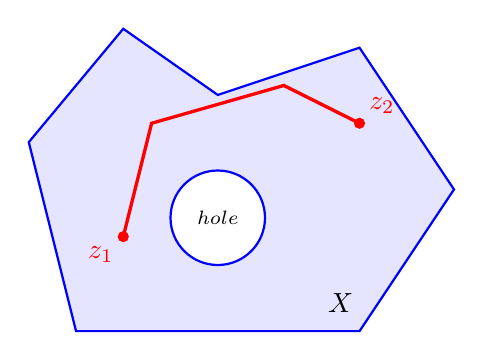
\begin{tikzpicture}[scale=1.2]
	
	% Outer non-convex boundary
	\fill[blue!10]
	(0,0) -- (3,0) -- (4,1.5) -- (3,3) -- (1.5,2.5) -- (0.5,3.2) -- (-0.5,2) -- (0,0) -- cycle;
	
	% Inner hole (not simply connected)
	\fill[white]
	(1.5,1.2) circle (0.5);
	
	% Outer boundary line
	\draw[thick,blue]
	(0,0) -- (3,0) -- (4,1.5) -- (3,3) -- (1.5,2.5) -- (0.5,3.2) -- (-0.5,2) -- (0,0) -- cycle;
	
	% Hole boundary
	\draw[thick,blue]
	(1.5,1.2) circle (0.5);
	
	% Two points in the region
	\filldraw[red] (0.5,1) circle (1.5pt) node[below left] {$z_1$};
	\filldraw[red] (3,2.2) circle (1.5pt) node[above right] {$z_2$};
	
	% Polygonal path connecting z1 to z2, avoiding the hole
	\draw[very thick,red]
	(0.5,1) -- (0.8,2.2) -- (2.2,2.6) -- (3,2.2);
	
	% Labels
	\node at (2.8,0.3) {$X$};
	\node at (1.5,1.2) {$\phantom{X}$};
	\node at (1.5,1.2) {$\scriptstyle\text{hole}$};
	
\end{tikzpicture}
\caption{A path-connected set}
\label{fig:path_connected_set}
	\end{center}
\end{figure}



\begin{svgraybox}
	\begin{theorem}
If a subset $X$ of $\mathbb{C}$ is path-connected, then it is connected (in the relative topology of $X$).
	\end{theorem}
\end{svgraybox}

\begin{proof}
	Suppose $X$ is path-connected. To show that $X$ is connected, we verify condition~(c) of 
	Theorem~\ref{thm:connected_set}.
	
	Assume that $X$ can be written as
	\[
	X = A \cup B,
	\]
	where $A$ and $B$ are disjoint, nonempty sets that are open in the relative topology of $X$.
	Choose points $z_1 \in A$ and $z_2 \in B$. Since $X$ is path-connected, there exists a path
	\[
	\gamma : [0,1] \to X
	\]
	such that $\gamma(0) = z_1$ and $\gamma(1) = z_2$.
	
	Consider the sets
	\[
	S \triangleq \gamma^{-1}(A), \qquad T \triangleq \gamma^{-1}(B).
	\]
	Because $A$ and $B$ are open in $X$ and $\gamma$ is continuous, both $S$ and $T$ are open in
	$[0,1]$ (with the relative topology). They are disjoint, and
	\[
	[0,1] = S \cup T,
	\]
	since every point of the path lies in either $A$ or $B$.	
	Moreover, $S$ and $T$ are both nonempty: $0 \in S$ because $\gamma(0)=z_1\in A$, and
	$1 \in T$ because $\gamma(1)=z_2\in B$.
	
	Thus we have written the interval $[0,1]$ as a union of two disjoint, nonempty, open subsets.
	But it is known from real analysis that the interval $[0,1]$ is connected, so such a
	decomposition is impossible.
	
	This contradiction shows that no such sets $A$ and $B$ can exist. Therefore $X$ cannot be
	written as the union of two disjoint nonempty open sets, and condition~(c) of
	Theorem~\ref{thm:connected_set} holds. Hence $X$ is connected.
\end{proof}

Convex set is a special kind of connected set.

\index{Convex set}
\begin{svgraybox}
	\begin{definition} \label{def:convex_set}
		A set $S$ in $\mathbb{C}$ is said to be \df{convex} if for any two points $z_1$ and $z_2$ in $S$, the line segment between $z_1$ and $z_2$ is in~$S$.
	\end{definition}
\end{svgraybox}

For example, a disk and a half-plane are convex, but a punctured disk and an annulus is not convex.



\begin{svgraybox}
	\begin{theorem}
Let $X$ be a nonempty open set in $\mathbb{C}$. Then $X$ is path-connected if it is connected. Moreover, we can always choose a polygonal path that connects two points in~$X$.
	\end{theorem}
\end{svgraybox}

\begin{proof}
	Let $X$ be a nonempty open and connected subset of $\mathbb{C}$. Fix a point $z_0 \in X$.
	We define
	\[
	Y \triangleq \{ z \in X : \text{there exists a polygonal path in $X$ from $z_0$ to $z$} \}.
	\]
	Clearly $z_0 \in Y$, so $Y$ is nonempty. We will show belowthat $Y$ is both open and closed in $X$.
%	By the connectedness of $X$, this will imply $Y = X$, and hence any point in $X$ can be joined
%	to $z_0$ by a polygonal path in $X$. This proves that $X$ is path-connected, and moreover that
%	we can always choose a polygonal path.
	
	\smallskip
	
	\noindent\textbf{($Y$ is open in $X$)}
	Let $z \in Y$. By definition, there is a polygonal path in $X$ from $z_0$ to $z$. Since $X$ is
	open, there exists $r>0$ such that the open disk $D(z,r)$ is contained in $X$.
	
	Take any $w \in D(z,r)$. Because $D(z,r)$ is convex, the line segment from $z$ to $w$ lies
	entirely in $D(z,r)$, and hence in $X$. Concatenating the polygonal path from $z_0$ to $z$
	with this line segment from $z$ to $w$ gives a polygonal path in $X$ from $z_0$ to $w$.
	Therefore $w \in Y$, and we have shown that $D(z,r) \subseteq Y$.
	Thus, for each $z \in Y$, there is a neighborhood of $z$ in $X$ contained in $Y$, so $Y$ is open in~$X$.
	
	\smallskip
	
	\noindent\textbf{($Y$ is closed in $X$)}
	We show that $X \setminus Y$ is open in $X$. Let $z \in X \setminus Y$. Since $X$ is open,
	there exists $r>0$ such that $D(z,r) \subseteq X$.
	
	We claim that $D(z,r) \cap Y = \emptyset$. Suppose, for contradiction, that there exists
	$w \in D(z,r) \cap Y$. Then, by definition of $Y$, there is a polygonal path in $X$ from
	$z_0$ to $w$. As before, the line segment from $w$ to $z$ lies entirely in $D(z,r)$, and hence
	in $X$. Concatenating the polygonal path from $z_0$ to $w$ with this line segment from $w$ to
	$z$ gives a polygonal path in $X$ from $z_0$ to $z$. This implies $z \in Y$, contradicting
	our assumption that $z \in X \setminus Y$.
	Therefore $D(z,r) \subseteq X \setminus Y$, so every point of $X \setminus Y$ has a
	neighborhood in $X$ contained in $X \setminus Y$. Hence $X \setminus Y$ is open in $X$, and
	so $Y$ is closed in~$X$.
	
	\smallskip
	
	\noindent\textbf{(Conclusion)}
	We have shown that $Y$ is nonempty, open, and closed in $X$. Since $X$ is connected, the only
	subsets of $X$ that are both open and closed are $\emptyset$ and $X$ itself. Thus we must have
	$Y = X$. Consequently, for any two points $z_1, z_2 \in X$, there is a polygonal path in $X$ from
	$z_1$ to $z_2$ (take the polygonal path from $z_0$ to $z_1$ and from $z_0$ to $z_2$, and
	concatenate appropriately). In particular, $X$ is path-connected, and the path can always be
	chosen to be polygonal.
\end{proof}


\begin{svgraybox}
	\begin{definition} \label{def:domain} \index{Domain} \index{Region}
A nonempty, open and connected set in $\mathbb{C}$ is referred to as 
a \df{domain} or \df{region}.
	\end{definition}
\end{svgraybox}




The followings are examples of domain.
\begin{itemize}
	\item Open disk $D(z_0,r)$.
	\item Punctured disk $D(z_0,r)\setminus \{z_0\}$.
	\item The complex plane $\mathbb{C}$.
	\item Annulus $\{z\in\mathbb{C}: a< |z| < b\}$.
	\item Open half-plane $\real(\alpha z)>0$, where $\alpha$ is a complex constant.
\end{itemize}






\section{Uniform convergence and continuity of power series}


The point-wise limit of a sequence of real-valued continuous functions needs not be a continuous function. A simple example is the sequence of function $x^k$, for $x\in[0,1]$. For $x$ that is strictly less than~1, the function $x^k$ converges to 0 as $k\rightarrow \infty$, but for $x=1$, the limit is 1  as $k\rightarrow \infty$.

%In general, we cannot exchange the order of integration and limit.

%\begin{example} (\cite[Section 7.6]{Rudin}) Consider the function $f_k(x) = k x(1-x^2)^k$, for $x\in [0,1]$, and $k=1,2,3,\ldots$. The pointwise limit of $f_k(x)$ is the zero function for $x\in[0,1]$, and hence 
%	$$\int_0^1 (\lim_{k\rightarrow\infty } f_k(x) )\, dx = 0.
%	$$
%	However, one can calculate that
%	$$
%	\int_0^1 f_k(x)\, dx = \int_0^1 k x(1-x^2)^k \, dx= \frac{k}{2k+2},
%	$$
%	which tends to a positive constant $1/2$ as $k\rightarrow\infty$ (See Fig.~\ref{fig:nonuniform_convergence}).
%\end{example} 

%\begin{figure}
%	\begin{center}
	%		\includegraphics[width=10cm]{nonuniform_convergence.PNG}
	%	\end{center}
%	\caption{Plot of function $nx(1-x^2)^n$ for $n=1,2,4,8,16,32,64$.}
%	\label{fig:nonuniform_convergence}
%\end{figure}


%If a sequence of continuous functions $f_k(x)$ converges uniformly, then the limit function $f(x)  = \lim_k f_k(x)$ is continuous, and we have
%$\int \lim_k f_k(x)\, dx = \lim_k \int f_k(x)\, dx$.

%The Stone-Weierstrass theorem says that given any continuous function $f(x)$ on an interval $[a,b]$, there exists a sequence of polynomial $p_k(x)$ that converges uniformly to $f(x)$. Since the continuous function $f(x)$ needs not be differentiable, it is not true in real analysis that the pointwise limit of a sequence differentiable functions is continuous, even if the convergence is uniform.

%For example, we take the function $f(x)=|x|$, for $x\in [-1,1]$. Then by Stone-Weiestrass approximation theorem, we can find a sequence of polynomial functions, which are all infinitely smooth, that converge to a function that is not differentiable at $x=0$. %In view of this example, the theorem of Weierstrass in Theorem~\ref{thm:Weierstrass} is remarkable.


We can guarantee that the limit function  is continuous if the convergence is uniform.


\begin{svgraybox}
	\begin{definition}\index{Convergence!uniform}
		A sequence of function $f_k(z)$ is said to be \df{uniformly converging} to a limit function $f(z)$ in a domain $D$ if for any $\epsilon>0$, we can find a sufficiently large index $N(\epsilon)$, which does not depend on $z$, such that
		$
		|f_k(z) - f(z)| \leq \epsilon$
		for all $k\geq N(\epsilon)$ and for all $z\in D$. \label{def:uniform_convergence_real}
	\end{definition}
\end{svgraybox}

We can show that $f_k(z)$ converge uniformly to $f(z)$ for $z\in D$ if and only if
\begin{equation}
	\lim_{k\rightarrow\infty} \big( \sup_{z\in D} |f_k(z) - f(z)| \big) = 0.
	\label{eq:alternate_uniform_convergence}
\end{equation}

\begin{svgraybox}
	\begin{theorem}
		Let $f_k(z)$ be a sequence of continuous functions defined in a domain $D$, for $k=1,2,\ldots$. If $f_k(z)$ converges to $f(z)$ uniformly in $D$, then $f(z)$ is continuous.
		\label{thm:uniform_convergence_continuous}
	\end{theorem}
\end{svgraybox}

\begin{proof}
	Pick a point $z_0$ in the domain $D$. For all $z\in D$ and for all $k\geq1$, we have
	$$
	|f(z) - f(z_0)| \leq 
	|f(z) - f_k(z)| + |f_k(z) - f_k(z_0)| + |f_k(z_0) - f(z_0)|,
	$$
	by triangle inequality. Since $f_k(z)$ converges uniformly, given any $\epsilon>0$, we can find two indices $N_1$ and $N_2$ such that $|f(z)-f_k(z)|\leq \epsilon /3$ for all $k\geq N_1$, and $|f_k(z_0) - f(z_0)|\leq \epsilon /3$ for all $k\geq N_2$. Let $k_0$ be an index larger than $\max(N_1,N_2)$. The middle term $|f_{k_0}(z) - f_{k_0}(z_0)|$ can be made arbitrarily small. More precisely, we can find $\delta>0$ such that $|f_{k_0}(z) - f_{k_0}(z_0)|\leq \epsilon /3$ whenever $|z-z_0|\leq \delta$.
	
	We put all the estimates together. Given any $\epsilon>0$, there is a $\delta>0$ such that
	$$
	|f(z)- f(z_0)| \leq \frac{\epsilon}{3}+\frac{\epsilon}{3}+\frac{\epsilon}{3} = \epsilon
	$$
	if $|z-z_0| \leq \delta$. This is exactly the definition of continuity at $z_0$.
\end{proof}


When applied to a series of functions, the condition of uniform convergence becomes:  for all $\epsilon >0$, there exists an integer $N(\epsilon)$ that depends only on $\epsilon$ but not on the value of $z$, such that
\begin{equation}
	\big| \sum_{k=1}^n g_k(z) - \sum_{k=1}^\infty g_k(z) z^k \big| <\epsilon
	\label{eq:uniform_convergence_power_series}
\end{equation}
for all $n \geq N(\epsilon)$ and for all $z$ in a domain $D$. The number $N(\epsilon)$ should be a function of $\epsilon$ only independent of~$z$.

%When applied to series, we say that a series of function $\sum_{k=1}^\infty g_k(z)$ converges {\em uniformly} to $g(z)$ if the sequence of partial sums
%$$
%f_n(z) = \sum_{k=1}^n g_k(z)
%$$
%converges to $g(z)$ uniformly as $n\rightarrow \infty$.
%

Weierstrass $M$ test is a convenient method to show that a series of functions converge uniformly.

\begin{svgraybox}
	\begin{theorem}[Weierstrass $M$ test] \index{Weierstrass $M$ test} \label{thm:M_test} Suppose $(g_k(z))_{k=1}^\infty$ is a sequence of  function defined on a domain $D$. If we can find positive real numbers $M_k$, for $k\geq 1$, such that
		
		(i) $|g_k(z)|\leq M_k$ for all $z\in D$, and
		
		(ii) $\sum_{k=1}^\infty M_k$ converges,
		
		then  $\sum_{k=1}^\infty g_k(z)$ converges uniformly in the domain~$D$. 
	\end{theorem}
\end{svgraybox}


\begin{proof}
	We first show that the sequence of function $g_k(z)$ converges. For any two indices $m<n$, we have
	\begin{equation}
		\big| \sum_{k=m+1}^n g_k(z) \big| \leq 
		\sum_{k=m+1}^n  |g_k(z)| \leq \sum_{k=m+1}^n M_k
		\label{eq:M_test_proof1}
	\end{equation}
	for all $z\in D$. Since $\sum_{k=1}^\infty M_k$ converges, given any $\epsilon >0$, we can find an index $N$ such that $\displaystyle \sum_{k=m+1}^n M_k$ is less than $\epsilon$  for all $m$ and $n$ larger than $N$. For this choice of $N$, we have 
	$$
	\Big| \sum_{k=m+1}^n g_k(z) \Big| \leq \epsilon
	$$
	for each $z\in D$. By Cauchy's criterion for convergence (Theorem~\ref{prop:Cauchy_sequence}), the limit of $g_k(z)$ as $k\rightarrow \infty$ exists for all $z$. We denote the limit function as~$g(z)$.
	
	Next, we show that the convergence is uniform. By triangle inequality, for all indices $m$ and $n$, 
	\begin{equation} \big|\sum_{k=1}^n g_k(z) - g(z)\big| \leq 
		\big|\sum_{k=1}^n g_k(z) - \sum_{k=1}^m g_k(z)\big| + \big|\sum_{k=1}^m g_k(z) - g(z)\big|.
		\label{eq:M_test_proof2}
	\end{equation}
	Given any $\epsilon>0$, using the argument in Equation~\eqref{eq:M_test_proof1}, we can find a larger index $N_\epsilon$, which only depends on $\epsilon$, such that $|\sum_{k=1}^n g_k(z) - \sum_{k=1}^m g_k(z)|\leq \epsilon/2$ for all $m,n\geq N$ and for all $z\in D$. 
	
	Moreover, since $g_k(z)$ converges to $g(z)$, there exists an integer $M(z,\epsilon)$, which depends on both $z$ and $\epsilon$, such that $|\sum_{k=1}^m g_k(z) - g(z)| \leq \epsilon/2$ for all $m\geq M(z,\epsilon)$. For each $z \in D$, we choose an integer $m(z)$ that is larger than $\max(M(z,\epsilon), N_\epsilon)$ (using axiom of choice). Then for all $z\in D$, we can conclude from \eqref{eq:M_test_proof2} that
	\begin{align*}
		\big|\sum_{k=1}^n g_k(z) - g(z)\big| 
		& \leq  \big|\sum_{k=1}^n g_k(z) - \sum_{k=1}^{m(z)} g_k(z)\big| + \big|\sum_{k=1}^{m(z)} g_k(z) - g(z)\big| \\
		& \leq \frac{\epsilon}{2} + \frac{\epsilon}{2} = \epsilon.
	\end{align*}
	for all $n\geq N_\epsilon$. This proves that $g_k$ converges to $g$ uniformly as $k\rightarrow\infty$.
\end{proof}





The following theorem shows that absolute convergence implies uniform convergence for power series.

\begin{svgraybox}
	\begin{theorem}
		Suppose  $\sum_{k=0}^\infty a_k z^k$ converges absolutely at $z=z_0$, then $\sum_{k=0}^\infty a_k z^k$ converges uniformly for $|z| \leq |z_0|$.
		\label{thm:uniform_convergence_circle}
	\end{theorem}
\end{svgraybox}


\begin{proof} 	For $k\geq 0$, let $M_k \triangleq |a_k| |z_0|^k$. By assumption, $\sum_{k=0}^\infty M_k$ converges. In addition, we have
	$$	
	|a_k z^k| \leq |a_k| |z_0|^k = M_k
	$$
	for all $z$ in the closed disk $|z|\leq |z_0|$.
	The result follows from Weierstrass $M$-test in Theorem~\ref{thm:M_test}.
	%	 Given any $\epsilon>0$, there exists an integer $N(\epsilon)$ such that
	%	$$
	%	\sum_{k=n+1}^\infty M_k \leq \epsilon, \qquad \text{ for all } n\geq N(\epsilon).
	%	$$
	%	So, for this choice of $N(\epsilon)$, we have
	%	\begin{align*}
		%		\Big| \sum_{k=0}^n a_k z^k - \sum_{k=0}^\infty a_k z^k\Big| &=
		%		\Big| \sum_{k=n+1}^\infty a_k z^k \Big| 
		%		\leq \sum_{k=n+1}^\infty |a_k| |z|^k 
		%		\leq \sum_{k=n+1}^\infty M_k \leq \epsilon
		%	\end{align*}
	%	for all $|z|\leq |z_0|$. This proves that $\sum_k a_k z^k$ is uniformly convergent to $\sum_{k=0}^\infty a_k z^k$ for $z$ in the closed disk $\{z:\, |z|\leq |z_0|\}$.
\end{proof}

\begin{svgraybox}
	\begin{theorem}
		The function defined by a power series is continuous in the region of convergence. \label{thm:power_series_continuous}
	\end{theorem}
\end{svgraybox}

\begin{proof}
	Suppose $R$ is the radius of convergence of a power series $\sum_{k=0}^\infty a_k z^k$. Let $z$ be a complex number with modulus $|z|$ strictly less than~$R$. Since $|z|<R$, we can find a real number $r$ between $|z|$ and $R$, e.g. we can take $r=(|z|+R)/2$. The power series $\sum_k a_k z^k$ is converging at $z=r$, and hence by Theorem~\ref{thm:uniform_convergence_circle}, the power series converges uniformly for $|z|\leq r$. Finally, we observe that the partial sum $\sum_{k=0}^n a_k z^k$ are polynomials for each natural number $n$, and is thus continuous. We see that the function defined by this power series is continuous at $z$. Since this argument works for all $|z|<R$, the function is continuous in the open disk $|z|<R$.
\end{proof}


We thus see that the functions defined by power series are all continuous.






\section*{Summary}

\begin{itemize}
\item The complex plane has the same topological properties of the Euclidean plane $\mathbb{R}^2$.

\item A function $f(z)$ is continuous at $z_0$ if  (i) $f(z_0)$ exists, (ii) $\lim_{z\rightarrow z_0} f(z)$ exists, and (iii) $\lim_{z\rightarrow z_0} f(z) = f(z_0)$.

\item The continuity of a complex function at the point at infinity can be seen from the continuity of $f(1/z)$ at $z=0$.

\item A path in the complex plane is represented parametrically by a continuous function $\gamma: [a,b] \rightarrow \mathbb{C}$.

\item A set $X$ is path-connected if any two points in $X$ are connected by a path in $X$.

\item A set $X$ is connected if it cannot be written as a union of two disjoint subsets that are relatively open in $X$.

\item When $X$ is connected, the only sets that are open and closed at the same time are the open set and $X$ itself. 

\item A domain is a nonempty, open and connected set in $\mathbb{C}$.

\item When $X$ is nonempty and open, path-connectedness is equivalent to connectedness.


\item A series $\sum_{k=1}^\infty g_k(z)$ converges  uniformly to $g(z)$ in a domain $D$ if for any $\epsilon >0$, there exists $N$ such that
$|\sum_{k=1}^n g_k(z) - g(z)| \leq \epsilon$ for all $n\geq N$ and for all $z\in D$.

\item The limit of a sequence of continuous functions is continuous if the convergence is uniform.


\item Weierstrass $M$ test is a tool that proves uniform convergence.

\item A function defined by power series is continuous in its region of convergence.

\end{itemize}


\section*{Exercises}
\renewcommand{\labelenumi}{\arabic{enumi}}
\begin{enumerate}
\item If $z_0$ is an accumulation point of a set $S\subseteq \mathbb{C}$ and $\lim_{z\rightarrow z0} f(z) = w$, then the limit is unique. \label{exercise:unique_limit}

\item Prove the usual rules for computing with limits of functions. Suppose $f(z)$ and $g(z)$ are complex function with limits $\lim_{z\rightarrow z_0} f(z) = w_1$ and $\lim_{z\rightarrow z_0} g(z) = w_2$. Show that
\begin{enumerate}
	\item $\lim_{z\rightarrow z_0} (f(z)+g(z)) = w_1+w_2$;
	\item $\lim_{z\rightarrow z_0} (f(z)-g(z)) = w_1-w_2$;
	\item $\lim_{z\rightarrow z_0} (f(z)g(z)) = w_1w_2$;
	\item $\lim_{z\rightarrow z_0} (f(z)/g(z)) = w_1/w_2$ (when $w_2\neq 0$).
\end{enumerate}

\item \label{exercise:continuous_preimage} Prove Theorem~\ref{thm:continuous_preimage}.

\item Prove that the trajectory of a path is  compact.

\item Show that the condition in \eqref{eq:alternate_uniform_convergence} is equivalent to the definition of uniform convergence in Definition~\ref{def:uniform_convergence_real}.


\end{enumerate}



%%%%%%%%%%%%%%%%%%%%%%%%%%%%%%%%%%%%%%%%%%%%%%% Lecture 6

\chapter{Complex Differentiability}

In this chapter we investigate the meaning that a complex function is differentiable at a point.

%In order to compute the derivative of a function at a point, we need to make a small difference in the domain and investigate the resulting change in the function value. In order to be able to have enough elbow room, we usually assume that the complex function is defined in an open set. 




\section{Differentiable real functions from multi-variable calculus}

When a real-valued function $f(x)$ is differentiable at a point $x_0$, we can approximate the function near $x_0$ by a linear function 
$$L(x) = f(x_0)+ f'(x_0)(x-x_0).
$$ The value of $f'(x_0)$ has the geometric meaning of slope in the graph of $f(x)$. 

Now consider a real-valued function $f(x,y)$ in variables $x$ and $y$. If $f(x,y)$ is differentiable at a point $(x_0,y_0)$, we can approximate $f(x,y)$ near $(x_0,y_0)$ by a linear function 
$$ L(x,y) = f(x_0,y_0) + \alpha (x-x_0)+ \beta(y-y_0),
$$
where $\alpha = f_x(x_0,y_0)$ and $\beta = f_y(x_0,y_0)$ are the partial derivatives of $f(x,y)$ with respect to $x$ and $y$, respectively, at the point $(x_0,y_0)$.
We can write the linear function $L(x,y)$ as
$$
L(x,y) = f(x_0,y_0) + 
\begin{bmatrix}
	f_x(x_0,y_0) & f_y(x_0,y_0)
\end{bmatrix}
\begin{bmatrix}
	x-x_0 \\ y-y_0
\end{bmatrix}.
$$
The vector 
$\begin{bmatrix}
	f_x(x_0,y_0) & f_y(x_0,y_0)
\end{bmatrix}$
is called the gradient of $f$ at $(x_0,y_0)$. We can express the linear approximation in terms of the differences,
$\Delta_x \triangleq x-x_0$ and $\Delta_y \triangleq y-y_0$,
$$
L(x_0+\Delta_x,y_0+\Delta_y) = f(x_0,y_0) + 
\begin{bmatrix}
	f_x(x_0,y_0) & f_y(x_0,y_0)
\end{bmatrix}
\begin{bmatrix}
	\Delta_x \\ \Delta_y
\end{bmatrix}.
$$

Next, we consider a vector-valued function 
$$\mathbf{F}(x,y) = (u(x,y), v(x,y)),
$$ 
which is also called a {\em vector field}. Differentiation of vector field is about linear approximation.

\begin{svgraybox}
	\begin{definition} \index{Real differentiable}
A vector-valued function $\mathbf{F}(x,y)\triangleq (u(x,y), v(x,y))$ is said to be \df{real differentiable} at a point $(x_0,y_0)$ in the domain of $\mathbf{F}$ if there exists a $2\times 2$ matrix $A$ such that 
\begin{equation}
	\begin{bmatrix} u(x_0+\Delta x, y_0+\Delta y) \\ v(x_0+\Delta x, y_0 + \Delta y) \end{bmatrix} 
\doteq
\begin{bmatrix} u(x_0,y_0) \\ v(x_0,y_0) \end{bmatrix}	+
	 A \cdot
	\begin{bmatrix} \Delta x \\ \Delta y \end{bmatrix}
	\label{eq:real_differentiable}
\end{equation}
when $(\Delta x, \Delta y)$ is small.
	\end{definition}
\end{svgraybox}

The symbol ``$\doteq$'' means that the difference between the left and right side of~\eqref{eq:real_differentiable} converges to zero faster than the linear term, i.e.,
\begin{equation}
\lim_{(\Delta x, \Delta y)\rightarrow (0,0)} \frac{\| \text{Difference between L.H.S and R.H.S. of \eqref{eq:real_differentiable}}\|}{\sqrt{\Delta x^2 + \Delta y^2}} =0.
\label{eq:real_differentiable2}
\end{equation}

The matrix $A$ is called the {\em total derivative} of $\mathbf{F}$ at $(x_0,y_0)$, if $\mathbf{F}$ is real differentiable at $(x_0,y_0)$. 


It is known that if $\mathbf{F}(x,y)$ is real differentiable at $(x_0,y_0)$, the partial derivatives of $u(x,y)$ and $v(x,y)$ exists at $(x_0,y_0)$, and the total derivative equals
$$
\begin{bmatrix} u_x(x_0,y_0) & u_y(x_0,y_0) \\ v_x(x_0,y_0) & v_y(x_0,y_0) \end{bmatrix}.
$$
The entries in the $2\times 2$ matrix are the partial derivatives of $u$ and $v$ evaluated at $(x_0,y_0)$ \cite[Theorem 9.17]{Rudin}. 
It is important to note that the mere existence of the partial derivatives of $\mathbf{F}$ is not sufficient to guarantee that \eqref{eq:real_differentiable} holds. The existence of of partial derivatives is a necessary condition of real differentiability.

In general, we have the following sufficient condition for real differentiability, which is easier to check \cite[Theorem 9.21]{Rudin}.

\renewcommand{\labelenumi}{(\roman{enumi}).}
\begin{svgraybox} 		\label{thm:real_sufficient}
	\begin{theorem} A vector field $\mathbf{F}(x,y) = (u(x,y), v(x,y))$ is real differentiable at a point $(x_0,y_0)$ if 
\begin{enumerate}
\item partial derivatives $u_x$, $u_y$, $v_x$ and $v_y$ exists in a neighborhood of $(x_0,y_0)$, and 
\item the partial derivatives $u_x$, $u_y$, $v_x$ and $v_y$ are continuous at $(x_0,y_0)$ in this neighborhood.
\end{enumerate}
	\end{theorem}
\end{svgraybox}



\begin{example}
	The function $\mathbf{F}(x,y)$ defined by $(x^2y, x+y)$ is real differentiable. Partial derivatives of the first component $u(x,y)=x^2y$ and the second component $v(x,y)=x+y$ exist, and are all continuous. Therefore $F$ is real differentiable, 	
	 and we have
	\begin{equation}
		\begin{bmatrix}(x_0+\Delta x)^2 (y_0 + \Delta y)\\ x_0+\Delta x + y_0 + \Delta y \end{bmatrix}
		\doteq
		\begin{bmatrix}x_0^2 y_0 \\ x_0+y_0 \end{bmatrix} +
		\begin{bmatrix} 2x_0y_0 & x_0^2 \\ 1 & 1 \end{bmatrix}
		\begin{bmatrix} \Delta x \\ \Delta y \end{bmatrix}
	\end{equation}
	for any $x_0$ and $y_0$.
	\label{ex:5A}
\end{example}

A classic example  that has partial derivatives but not differentiable.
\begin{example} \label{ex:non_differential_vector_function}
Let $F(x,y)$ be the vector field defined by
$$
\mathbf{F}(x,y) \triangleq 
\begin{cases}
\big( \frac{x^2y}{x^2+y^2}, \frac{xy^2}{x^2+y^2} \big)	& \text{if } (x,y)\neq (0,0) , \\
0 & \text{if } (x,y)=(0,0).
\end{cases}
$$
Let $u$ and $v$ denote the first and the second components of $\mathbf{F}(x,y)$
The partial derivatives $u_x$, $y_y$, $v_x$, $v_y$ at the origin exist and are all equal to 0, but $\mathbf{F}$ is not real differentiable at the origin. It is not differentiable because if we approach the origin along the straight line $x=y$, the value of $F(x,x)$ equals $(x/2,x/2)$, so that
$$
\lim_{x\rightarrow 0}\frac{\| \mathbf{F}(x,x)\| }{\sqrt{2x^2}} = \frac{1}{2},
$$
contradicting the defining condition in \eqref{eq:real_differentiable2} that the limit should be~0.
\end{example}


\section{Complex differentiability and Cauchy-Riemann condition}

After the revision of differentiation in multi-variable calculus, we now consider a complex function $f(z)$ as a two-dimensional vector field,
$$
f(x+iy) = u(x,y) + i v(x,y).
$$
and study $f(z)$ as if it is a vector field. We motivate the notion of complex differentiability by an example.

\begin{example} 	\label{ex:complex_differentiation_z_cube}
	Consider the function $$f(z)=z^3 = (x+iy)^3 = (x^3-3xy^2) + i (3x^2y-y^3).$$
	The real and imaginary parts are $u(x,y) = x^3-3xy^2$ and $v(x,y) = 3x^2y-y^3$, respectively. The partial derivatives of $u$ and $v$ are
	\begin{align*}
		u_x(x,y) &= 3x^2-3y^2 ,\\
		u_y(x,y) &= -6xy, \\
		v_x(x,y) &= 6xy, \\
		v_y(x,y) &= 3x^2 -3y^2.
	\end{align*}
	
	Suppose we fix a base point $(x_0,y_0)=(2,1)$. The linear approximation in~\eqref{eq:real_differentiable} at $(2,1)$ can be written as
	$$
	\begin{bmatrix}u(2+\Delta x, 1+\Delta y) \\ v(2+\Delta x, 1 + \Delta y) \end{bmatrix}
	\doteq
	\begin{bmatrix}2\\11 \end{bmatrix} +
	\begin{bmatrix} 9&-12 \\ 12 &9 \end{bmatrix}
	\begin{bmatrix} \Delta x \\ \Delta y \end{bmatrix}.
	$$
	For general $z=x+iy$, the $2\times 2$ matrix consisting of the partial derivatives is
	$$
	\begin{bmatrix}
		3x^2-3y^2 & -6xy \\ 6xy & 3x^2-3y^2
	\end{bmatrix}.
	$$
	The total derivative is in the form as in the matrix representation of complex number (Sec.~\ref{sec:complex_numbers_matrices}). 
	We can use simplify the linear approximation in terms of complex variable,
	\begin{align*}
		f(z+\Delta z) &= f(z) + (3x^2-3y^2 +i(6xy))\cdot (\Delta x + i \Delta y) \\
		&= f(z) + (3z^2)\Delta z.
	\end{align*}
\end{example}

\begin{svgraybox}
\begin{definition} \index{Complex differentiable} 	\label{def:complex_differentiable} Let $f(z)$ be a complex function defined in a domain $D$. Given a point $z_0\in D$, we say that $f$ is \df{complex differentiable at $z_0$} if there exists a complex constant $w_0$ such that 
	\begin{equation}
	f(z_0 + \Delta z) \doteq f(z_0) + w_0 \cdot \Delta z.
	\label{eq:complex_derivative1}
\end{equation}	
The constant $w_0$ is called the derivative of $f(z)$ at $z_0$, and is denoted by $f'(z_0)$.
\end{definition}
\end{svgraybox}

The symbol $\doteq$ in \eqref{eq:complex_derivative1} means 
$$
f(z_0 + \Delta z) = f(z_0) + w_0 \cdot \Delta z + o(\Delta z),
$$
where $o(\Delta z)$ represents a function that satisfies 
\begin{equation}
	\lim_{\Delta z \rightarrow 0} \frac{|o(\Delta z)|}{|\Delta z|} = 0.
	\label{eq:complex_derivative_limit0}
\end{equation}

In some textbooks, the following equivalent condition is adopted as the definition of complex differentiability.

\begin{svgraybox}
	\begin{theorem} 
Let $f(z)$ be a complex function defined  an a domain $D$ and $z_0$ is a point in $D$.	Then $f(z)$ is complex differentiable at $z_0$ if and only if the limit 
		\begin{equation}
			\lim_{h \rightarrow 0} \frac{f(z_0+h) -f(z_0)}{h}
			\label{eq:complex_derivative_limit}
		\end{equation}
		exists. 
	\end{theorem}
\end{svgraybox}

\begin{proof}
($\Rightarrow$) Suppose $f(z)$ is complex differentiable at $z_0$, then the complex constant $w_0$ is precisely the limit in \eqref{eq:complex_derivative_limit0}. We can see this by re-writing the fraction in \eqref{eq:complex_derivative_limit0},
$$
\frac{|o(\Delta z)|}{|\Delta z|} =
\frac{|f(z_0+\Delta z) - f(z_0) - w_0 \cdot \Delta z)|}{|\Delta z|} \stackrel{(a)}{=}
\Big| \frac{f(z_0+\Delta z) - f(z_0) - w_0 \cdot \Delta z)}{\Delta z} \Big|
$$
The assumption that this has limit  zero  as $\Delta z\rightarrow 0$ is the same as saying
$$
\lim_{\Delta z\rightarrow 0} \frac{f(z_0+\Delta z) - f(z_0) - w_0 \cdot \Delta z}{\Delta z} = 0, 
$$
which is then equivalent to
$$
\lim_{h \rightarrow 0} \frac{f(z_0+h) - f(z_0)}{h} = w_0. 
$$

($\Leftarrow$) The steps in the previous paragraph are all reversible. Starting from the assumption that the limit $\lim_{h\rightarrow 0} \frac{f(z_0+h) - f(z_0)}{h}$ exists and equal to $w_0$, we can deduce 
$$
\lim_{\Delta z\rightarrow 0} \frac{|f(z_0+\Delta z) - f(z_0) - w_0 \cdot \Delta z)|}{|\Delta z|} = 0.
$$
This proves that the two definitions are equivalent to each other.
\end{proof}


We note that the step (a) in the previous proof is the following elementary fact about complex modulus:
$$
\Big| \frac{z_1}{z_2} \Big| = \frac{|z_1|}{|z_2|}.
$$



Immediately from Definition~\ref{eq:complex_derivative1}, we have a necessary condition for complex differentiability.
\index{Cauchy-Riemann condition}
\begin{svgraybox}
	\begin{theorem}[Cauchy-Riemann condition] 	\label{thm:CR}
		Suppose $f(x+iy) = u(x,y)+i v(x,y)$ is complex differentiable at $z_0=x_0+iy_0$ (see Definition \ref{def:complex_differentiable}), where $z_0$ is in the domain of $f(z)$. Then the partial derivatives $u_x$, $u_y$, $v_x$ and $v_y$ at $z_0$ exist, and they satisfy
		$$
		u_x(x_0,y_0) = v_y(x_0,y_0),\ \ \text{ and } \ \ u_y(x_0,y_0) = -v_x(x_0,y_0).
		$$
	\end{theorem}
\end{svgraybox}

The concept of complex differentiability is thus the same as
$$
	\boxed{\textrm{Complex differentiability} = \textrm{Real differentiability } +  \textrm{Cauchy-Riemann condition}}
$$
We formalize this in the form of a theorem.

\renewcommand{\labelenumi}{(\roman{enumi}).}
\begin{svgraybox}
	\begin{theorem}
		Suppose $f(z) = u(x, y)+iv(x, y)$ is a complex function defined on a domain $D$ which
		contains $z_0 = x_0 + iy_0$. Then, the limit 
$$
\lim_{h\rightarrow 0} \frac{f(z_0+h) - f(z_0)}{h}
$$		
		exists
		if and only if 
\begin{enumerate}
	\item the vector function $(u(x, y), v(x, y))$ is real-differentiable at $(x_0, y_0)$,
	\item   the partial derivatives satisfy the Cauchy-Riemann equations
	$
	u_x = v_y$, $u_y = -v_x$ at $(x_0,y_0)$.
\end{enumerate}		
		 \label{thm:complex_differentiable_equivalent_condition}
	\end{theorem}
\end{svgraybox}

We give a self-contained proof of this theorem in the appendix of this chapter.

\begin{example}
	For any complex constant $a$, the function $f(z) = az$ is complex differentiable at every point $z_0$ in $\mathbb{C}$, i.e., it is complex differentiable at every point in the complex plane, and the derivative is equal to $a$. We can see this by checking the definition of complex derivative.
	$$
	\Big| \frac{a(z_0 +h) - az_0}{h} - a\Big|= 0.
	$$
	We have $\frac{a(z_0 +h) - a z_0}{h} =a$ for all nonzero $h\in\mathbb{C}$. If we take limit, the limit is equal to~$a$. We have thus proved that the complex derivative of the linear function $f(z)=az$ is equal to a constant~$a$.
	
	Likewise, we can see that the derivative of a translation function $z\mapsto z+b$ is complex differentiable, and the derivative is equal to~1.
	\label{}
\end{example}

\begin{example}
	Let $f(z) = 1/z$ be the inversion function. We will show that this function is complex differentiable at all nonzero $z_0$ from definition. For $z_0\neq 0$,
	\begin{align*}
		\frac{\frac{1}{z_0+h} - \frac{1}{z_0}}{h} &=
		\frac{1}{h}\Big( \frac{z_0-(z_0+h)}{(z_0+h)z_0}\Big) \\
		&= - \frac{1}{z_0(z_0+h)}.
	\end{align*}
	When $h\rightarrow 0$, the limit  of $- \frac{1}{z_0(z_0+h)}$ is $-1/z_0^2$. Therefore $f(z)=1/z$ is complex differentiable for $z\in\mathbb{C}\setminus\{0\}$, and the complex derivative is $-1/z_0^2$.
	\label{ex:holomorphic_example4}
\end{example}


The function in Example \ref{ex:5A} is real differentiable everywhere but not complex differentiable. As a matter of fact, the function in Example~\ref{ex:5A} fails the Cauchy-Riemann equation for all real numbers $x_0$ and $y_0$, and thus is not complex differentiable anywhere. The following is a primary example that is real differentiable function but not complex differentiable.

\begin{example}
	The conjugate function $f(z) = \bar{z}$ is not complex differentiable anywhere. It is because $u_x=1$ and $v_y=-1$, and $u_x\neq v_y$ at any point in $\mathbb{C}$. It fails the Cauchy-Riemann equations everywhere.
	\label{ex:holomorphic_example2}
\end{example}

Since checking real differentiability by definition is not easy in general, we can use Theorem~\ref{thm:real_sufficient} to provide a sufficient condition for complex differentiability. 

\renewcommand{\labelenumi}{(\roman{enumi}).}
\begin{svgraybox}
	\begin{theorem}[A sufficient condition for complex differentiability]
		A complex function $f$ is complex differentiable at $z_0$ if
		\begin{enumerate}
			\item The partial derivatives $u_x$, $u_y$, $v_x$, $v_y$ exists in a neighborhood of $z_0$;
			\item $u_x$, $u_y$, $v_x$, $v_y$  are continuous at $z_0$;
			\item Cauchy-Riemann equations are satisfied at $z_0$.
		\end{enumerate}
		%	If the above conditions hold, the complex derivative of $f$ is given by $u_x+i v_x = v_y - iu_y$.
		\label{thm:complex_differentiable}
	\end{theorem}
\end{svgraybox}



As in the real case, complex differentiability implies continuity.

\begin{svgraybox}
	\begin{theorem}
		If $f(z)$ is complex differentiable at $z_0$, then $f(z)$ is continuous at~$z_0$.
	\end{theorem}
\end{svgraybox}

\begin{proof}
	Suppose $f(z)$ is complex differentiable at $z_0$. By the definition of complex differentiability, we can find a complex number $w_0$ such that 
	$$
	f(z_0+h) = f(z_0) + w_0 \cdot h + o(h), 
	$$
	where $h$ is a complex variable and $o(h)$ is a function with the property that $|o(h)/h|\rightarrow 0$ as $h\rightarrow 0$. If we do not divide by $h$, the function $o(h)$ converges to zero as well, because
	$$
	\lim_{h\rightarrow 0} o(h) = 
	\lim_{h\rightarrow 0} \frac{o(h)}{h} h = 
	\lim_{h\rightarrow 0} \frac{o(h)}{h} \cdot \lim_{h\rightarrow 0} h = 0\cdot 0=0.
	$$
	Therefore 
	$$
	\lim_{h\rightarrow 0} f(z_0+h) = f(z_0)
	+ \lim_{h\rightarrow 0} w_0 \cdot h + 
	\lim_{h\rightarrow 0} o(h) = f(z_0).
	$$
This matches the definition of continuity of a function at a point in Definition~\ref{def:continuous_function}.
\end{proof}

The following formulae are useful in calculating complex derivative.

\begin{svgraybox}
	\begin{theorem} \label{cor:CR}
		If a complex function $f(z) = u(x,y)+iv(x,y)$ is complex differentiable at $z_0 = x_0+iy_0$, the complex derivative at $z_0$ can be computed by
\begin{equation}
	f'(z_0) = 	u_x(x_0,y_0) + i v_x(x_0,y_0),
\label{eq:derivative_formula1}
\end{equation}
		or
\begin{equation}
	f'(z_0) = 	v_y(x_0,y_0) - i u_y(x_0,y_0).
\label{eq:derivative_formula2}		
\end{equation}
	\end{theorem}
\end{svgraybox}




\begin{proof}
	Let $f$ be a complex function that is complex differentiable at $z_0 = x_0+iy_0$. The limit in \eqref{eq:complex_derivative_limit} that defines the complex derivative does not depend on how we approach the point $z_0$. We can approach $z_0$ horizontally or vertically, and the results must be the same if the function is complex differentiable. 

	Let $\Delta z= \Delta x$ and take $\Delta x\rightarrow0$.
	\begin{align*}
		& \phantom{=} \lim_{\Delta x\rightarrow 0} \frac{u(x_0+\Delta x,y_0)+iv(x_0+\Delta x,y_0)-u(x_0,y_0)-iv(x_0,y_0)}{\Delta x} \\
		&=\lim_{\Delta x\rightarrow 0} \frac{u(x_0+\Delta x,y_0)-u(x_0,y_0)}{\Delta x}
		+ i\lim_{\Delta x\rightarrow 0} \frac{v(x_0+\Delta x,y_0)-v(x_0,y_0)}{\Delta x} \\ 
		&= \frac{\partial u}{\partial x}(x_0,y_0) + i \frac{\partial v}{\partial x}(x_0,y_0).
	\end{align*}
This proves that $$f'(z_0) = 	u_x(x_0,y_0) + i v_x(x_0,y_0).$$
	
	Next suppose $\Delta z= i \Delta y$ and take $\Delta y\rightarrow0$.
	\begin{align*}
		& \phantom{=} \lim_{\Delta y\rightarrow 0} \frac{u(x_0,y_0+\Delta y)+iv(x_0,y_0+\Delta y)-u(x_0,y_0)-iv(x_0,y_0)}{i \Delta y} \\
		&=\lim_{\Delta y\rightarrow 0} \frac{u(x_0,y_0+\Delta y )-u(x_0,y_0)}{i \Delta y}
		+ i\lim_{\Delta y\rightarrow 0} \frac{v(x_0,y_0+\Delta y)-v(x_0,y_0)}{i \Delta y} \\ 
		&= - i\frac{\partial u}{\partial y}(x_0,y_0) +  \frac{\partial v}{\partial y}(x_0,y_0).
	\end{align*}
We obtain
$$
f'(z_0) = 	v_y(x_0,y_0) - i u_y(x_0,y_0).
$$
\end{proof}	


\begin{example}
The identity function $f(z)=z$ is complex differentiable at all points in $\mathbb{C}$, and the derivative is constantly equal to 1.  We can check it using \eqref{eq:complex_derivative_limit}. For any $z_0\in\mathbb{C}$,
$$
 \lim_{h\rightarrow 0} \frac{f(z_0+h)-f(z_0)}{h} = 
 \lim_{h\rightarrow 0}  \frac{z_0+h-f(z_0)}{h} = \lim_{h\rightarrow 0} 1 = 1.
$$
\end{example}

\begin{example}
Consider the square function 
$$f(z)=z^2 = (x+iy)^2 = x^2-y^2 +i (2xy).
$$
We check that the Cauchy-Riemann condition are satisfied:
\begin{align*}
	u_x &= 2x = v_y \\
	u_v &= -2y = -v_x 
\end{align*}
Since the partial derivatives are continuous for all $x$ and $y$, by Theorem~\ref{thm:complex_differentiable}, the square function $z\mapsto z^2$ is complex differentiable. The derivative is
$$ 
2x + i (2y) = 2z
$$
by \eqref{eq:derivative_formula1}. \label{ex:holomorphic_example3}
\end{example}

\begin{example} \label{ex:holomorphic_example6}
The complex exponential function 
$$
e^z = e^x\cos y + i e^x \sin y  = u(x,y) + i v(x,y)
$$
is complex differentiable.  We compute the partial derivatives of the real and imaginary parts:
\begin{flalign*}
&&	u_x &= e^x\cos y, &u_y &= -e^x \sin y, &
	v_x &= e^x\sin y, &v_y &= e^x \cos y. &&
\end{flalign*}
The partial derivatives satisfy the Cauchy-Riemann equation, and are all continuous. Therefore, by Theorem~\ref{thm:complex_differentiable}, the complex exponential function is complex differentiable at every point on the complex plane. Applying~\eqref{eq:derivative_formula1}, the derivative is 
$$
f'(z) = u_x + iv_x = e^x \cos y + i e^x \sin y = e^z.
$$
\end{example}

Following the same strategy as in the previous example, we can prove that $\sin z$, $\cos z$, $\sinh z$, $\cosh z$ are complex differentiable at all points on $\mathbb{C}$.

\begin{svgraybox}
	\begin{theorem}  \label{thm:differentiable_compose}
Suppose $f$ is complex differentiable at $z_0$ and $g$ is complex differentiable at $f(z_0)$. Then the composition function $g\circ f$ is complex differentiable at~$z_0$.
	\end{theorem}
\end{svgraybox}

\begin{proof}
We leverage the fact from real analysis that the composition of real differentiable functions are real differentiable. Let $u(x,y)$ and $ v(x,y)$ be the real and imaginary parts of $f(z)$. The assumption that $f(z)$ is differentiable at $z_0 = x_0+iy_0$ means that we have the linear approximation
$$
	\begin{bmatrix} u(x_0+\Delta x, y_0+\Delta y) \\ v(x_0+\Delta x, y_0 + \Delta y) \end{bmatrix} 
\doteq
\begin{bmatrix} u(x_0,y_0) \\ v(x_0,y_0) \end{bmatrix}	+
\begin{bmatrix}
a & -b \\ b & a
\end{bmatrix} \cdot
\begin{bmatrix} \Delta x \\ \Delta y \end{bmatrix},
$$
for some real constants $a$ and $b$. Suppose $f(z_0) = r_0 + i s_0$, and $g(z)$ is complex differentiable at $f(z_0)$. Denote the real and imaginary parts of $g(z)$ by $\mu(r,s)$ and $\nu(r,s)$. We approximate $g$ near $(r_0,s_0)$ by
$$
\begin{bmatrix} \mu(r_0+\Delta r, s_0+\Delta s) \\ \nu(r_0+\Delta r, s_0 + \Delta s) \end{bmatrix} 
\doteq
\begin{bmatrix} \mu(r_0,s_0) \\ \nu(r_0,s_0) \end{bmatrix}	+
\begin{bmatrix}
	c & -d \\ d & c
\end{bmatrix} \cdot
\begin{bmatrix} \Delta r \\ \Delta s \end{bmatrix},
$$
for some constants $c$ and $d$. 

By  \cite[Theorem 9.15]{Rudin}, The composed function $g \circ f$ is real differentiable at $(x_0,y_0)$, 
$$
\begin{bmatrix} \real(g\circ f)(x_0+\Delta x, y_0+\Delta y) \\ \imag(g\circ f)(x_0+\Delta x, y_0 + \Delta y) \end{bmatrix} 
\doteq
\begin{bmatrix} \real(g\circ f) (x_0,y_0) \\ \imag(g\circ f) (x_0,y_0) \end{bmatrix}	+ \begin{bmatrix}
	c & -d \\ d & c
\end{bmatrix} \cdot
\begin{bmatrix}
	a & -b \\ b & a
\end{bmatrix} \cdot
\begin{bmatrix} \Delta x \\ \Delta y \end{bmatrix}.
$$
The product of the two matrices are in the from 
$$
\begin{bmatrix}
	\alpha & -\beta \\ \beta & \alpha
\end{bmatrix}.
$$
Hence, the Cauchy-Riemann condition is satisfied for the composition $g(f(z))$ at $z_0$. By Theorem~\ref{thm:complex_differentiable_equivalent_condition}, $g(f(z))$ is complex differentiable at~$z_0$.
\end{proof}



\section{Complex differential form and Wirtinger derivatives}
We give a characterization of complex differentiability using differential form.
The main reference of this section are \cite[Chapter 5]{Spivak} and \cite[Chapter 1]{ChernChenLam}.

In calculus, a differential $dx$ is usually regarded as an infinitesimal quantity, representing a very small change in the $x$ variable. The {\em total differential} of a bi-variate function $f(x,y)$ is 
$$
df = \frac{\partial f}{\partial x} dx + \frac{\partial f}{\partial y} dy .
$$
However, the treatment of differential form in calculus is usually not very rigorous.

We study complex differentiability by first considering multi-variable real functions and give a more rigorous definition of differential $dx$ and $dy$. Then we extend it to the complex case and give a concrete meaning of the symbol $dz$. In the remainder of this section we will borrow some notation from real manifolds. However, we do not need the full generality but only need the special case of dimension 2 and when the manifold is flat.

\subsection{Vector field and differential form}
\label{sec:tangent_space}
We first consider the Euclidean space $\mathbb{R}^2$ in the real case.

We define the tangent space at a given a point $\mathbf{p}$ in $\mathbb{R}^2$ as the set of all vectors that emanate from $\mathbf{p}$. The center point is represented by a position vector $\mathbf{p}$. To emphasize the starting point of a tangent vector, we write
$$
(\mathbf{p}, \mathbf{v})
$$
to represent a tangent vector emanating from the point $\mathbf{p}$. As an alternate notation, we will also write $\mathbf{v}_\mathbf{p}$ to mean a vector $\mathbf{v}$ with initial point $\mathbf{p}$.





The first component, $\mathbf{p}$, indicates that $\mathbf{p}$ is the initial point. We can add two vectors in $T_\mathbf{p}$ as follows,
$$
(\mathbf{p}, \mathbf{v}_1) + (\mathbf{p}, \mathbf{v}_2) \triangleq (\mathbf{p}, \mathbf{v}_1 + \mathbf{v}_2 )  
$$
and multiply by a scalar
$$
a(\mathbf{p}, \mathbf{v}) \triangleq (\mathbf{p}, a\mathbf{v}).
$$
However, if $\mathbf{p}$ and $\mathbf{q}$ are two distinct vector, the addition of $(\mathbf{p}, \mathbf{u})$ and $(\mathbf{q}, \mathbf{v})$ are not defined. Dot product of two vectors in $T_\mathbf{p}$ is done in the natural way
\begin{equation}
	(\mathbf{p}, \mathbf{u}) \cdot  (\mathbf{p}, \mathbf{v})  \triangleq
	 \mathbf{u} \cdot \mathbf{v}.
	\label{def:tangent_vector_dot_product}
\end{equation} (See Fig.~\ref{fig:tangent_space})

\begin{svgraybox}
	\begin{definition} \index{Tangent space}
		Given a point $\mathbf{p}$, the \df{tangent space at $\mathbf{p}$} is defined as the set
		$$
		T_\mathbf{p} \triangleq \{ (\mathbf{p}, \mathbf{v}):\, \mathbf{v} \in\mathbb{R}^2 \}.
		$$ 
	\end{definition}
\end{svgraybox}

For each point $\mathbf{p}$, the tangent space $T_\mathbf{p}$ is a two-dimensional vector space. We will use $\mathbf{e}_1$ and $\mathbf{e}_2$ to denote the standard basis. We will also use the shorter notation $\mathbf{v}_\mathbf{p}$ instead of $(\mathbf{p},\mathbf{v})$. The following is an example of computations in terms of the basis vectors $(\mathbf{e}_1)_\mathbf{p}$ and $(\mathbf{e}_2)_\mathbf{p}$,
$$
2 (4\mathbf{e_1}-\mathbf{e_2})_\mathbf{p} + (\mathbf{e_1}+ 3 \mathbf{e_2})_\mathbf{p} =(9\mathbf{e_1}+ \mathbf{e_2})_\mathbf{p}.
$$



\begin{figure}
	\begin{center}
\begin{tikzpicture}[scale=1.2, >=stealth]
	
	% Axes
	\draw[->] (-4,0) -- (4,0) node[right] {$x$};
	\draw[->] (0,-3) -- (0,3) node[above] {$y$};
	
	% Points
	\filldraw[black] (-2,1) circle (2pt) node[above left] {$\mathbf{p}$};
	\filldraw[black] (2,-1) circle (2pt) node[below right] {$\mathbf{q}$};
	
	% Vector field around P
	\foreach \angle in {0,30,...,330} {
		\draw[->,gray] (-2,1) -- ++(\angle:0.8);
	}
	
	% Vector field around F
	\foreach \angle in {0,30,...,330} {
		\draw[->,gray] (2,-1) -- ++(\angle:0.8);
	}
	
	\draw (-2,2) node {$\mathbf{v}_\mathbf{p}$};
	\draw (-1.1,1.5) node {$\mathbf{w}_\mathbf{p}$};	
	\draw (2.5,-1.9) node {$\mathbf{v}_\mathbf{q}$};
    \draw (1.2, -1.5) node {$\mathbf{u}_\mathbf{q}$};	
\end{tikzpicture}
	\end{center}
	\caption{Tangent space at point $\mathbf{p}$ and tangent space at $\mathbf{q}$}
	\label{fig:tangent_space}
\end{figure}

\begin{svgraybox}
	\begin{definition}
		A \df{smooth vector field} is a mapping that associates, for each point $\mathbf{p}$, a tangent vector $\mathbf{v}_\mathbf{p}$, in a continuous and smooth manner. 
	\end{definition}
\end{svgraybox}
For instance, we can represent a vector in each tangent space using a formula, such as
\begin{equation}
(a(x,y) \mathbf{e}_1 + b(x,y)\mathbf{e}_2)_{(x,y)} 
\label{eq:smooth_vector_field}
\end{equation}
for $(x,y) \in \mathbb{R}^2$, where $a(x,y)$ and $b(x,y)$ are smooth functions of $x$ and~$y$. In simple terms, the expression above says that at the point $(x,y)$, we select the vector $a(x,y) \mathbf{e}_1 + b(x,y)\mathbf{e}_2$ from the associated tangent space $T_{(x,y)}$. To further simplify notation, very often we skip the subscript~${}_{(x,y)}$. In physics notation, the two unit vectors are commonly denoted as $\vec{i}$ and $\vec{j}$. We can write $$a(x,y) \vec{i} + b(x,y)\vec{j},$$  representing a vector emanating from the point $(x,y)$, with horizontal and vertical components equal to $a(x,y)$ and $b(x,y)$, respectively. 

We now turn to the dual of vector space.

\begin{svgraybox}
	\begin{definition}
	Given a real vector space $V$, a  \df{covector} or \df{linear functional} is a linear function that takes a vector from $V$ as input and return a real number.
	\end{definition}
\end{svgraybox}
 When $V$ is $\mathbb{R}^2$, a typical example of covector is
$$
g_{a,b}(x,y) = ax+by,
$$
where $a$ and $b$ are fixed parameters of the linear functional $g_{a,b}$. For example the function
$$
(x,y) \mapsto x+y
$$
is a covector that returns the sum of the two coordinates, the function
$$
(x,y) \mapsto 2x-y
$$
is another covector. But the function
$$
(x,y)\mapsto xy
$$
is not a covector, because it is not a linear function.

In general, a linear functional $f(x,y)$ can be expressed as a dot product $(a,b)\cdot(x,y)$ for some constants $a$ and~$b$.

The set of all covectors of a vector space has the structure of vector space. We can add two covectors $g(x,y)$ and $h(x,y)$ according to the rule
$$
(g+h) (x,y) = g(x,y)+h(x,y),
$$
and multiply a covector $g$ by a scalar constant $a$ to obtain an new covector $ag$,
$$
(ag)(x,y) = a\cdot g(x,y).
$$
We will call this vector space the \df{dual space} of $V$. The notation of dual space is $V^*$.


When $V$ is isomorphic to $\mathbb{R}^2$, the dual space has dimension 2. We can take $\phi_1$ and $\phi_2$, defined by
\begin{align}
	\phi_1(x\mathbf{e}_1 + y\mathbf{e}_2) & \triangleq  x,
	\label{eq:phi1} \\
	\phi_2(x\mathbf{e}_1 + y\mathbf{e}_2) &\triangleq  y.
	\label{eq:phi2}
\end{align}
as a basis of $V^*$.

The next result shows that $\phi_1$ and $\phi_2$ span the vector space $(\mathbb{R}^2)^*$.

\begin{svgraybox}
	\begin{theorem} \label{thm:dual_space}
		Let $\phi_1$ and $\phi_2$ be the covectors \eqref{eq:phi1} and \eqref{eq:phi2}. 
		\begin{enumerate}
	\item	A linear combination
		$a\phi_1 + b \phi_2$, where $a$ and $b$ are real constants, is a covector in $(\mathbb{R}^2)^*$. 
	\item any covector in $(\mathbb{R}^2)^*$ can be written in the form $a\phi_1+b\phi_2$ for some real constants $a$ and $b$.
	\item $\phi_1$ and $\phi_2$ are linearly independent over $\mathbb{R}$.
		\end{enumerate}
		\end{theorem}
\end{svgraybox}

\begin{proof}
For any two constants $a$ and $b$, the function $a\phi_1+b\phi_2$ maps vector $x\mathbf{e}_1 + y \mathbf{e}_2$ to 
$$
a\phi_1(x\mathbf{e}_1 + y \mathbf{e}_2)+b\phi_2(x\mathbf{e}_1 + y \mathbf{e}_2) = a x + b y.
$$
This is a linear function from $\mathbb{R}^2$ to $\mathbb{R}$.

Next, consider a linear function $\theta: \mathbb{R}^2 \rightarrow \mathbb{R}$. We define 
$a \triangleq \theta(\mathbf{e}_1)$ and
$b \triangleq \theta(\mathbf{e}_2)$. 
For any vector $x\mathbf{e}_1 + y \mathbf{e}_2$, we have
$$
\theta(x\mathbf{e}_1 + y \mathbf{e}_2) = 
x \theta(\mathbf{e}_1)  + y \theta(\mathbf{e}_2) =
ax + by.
$$
We see that $\theta$ is equal to the linear combination $a\phi_1 + b \phi_2$ of $\phi_1$ and $\phi_2$.

To prove linear independence, suppose we can find two realk constants $\alpha$ and $\beta$ such that $\alpha \phi_1 + \beta \phi_2$ is the zero function. Then we must have both $\alpha$ and $\beta$ equal 0. We can see $\alpha=0$ by evaluating at $\mathbf{e}_1$,
$$
\alpha \phi_1(\mathbf{e_1}) + \beta \phi_2(\mathbf{e_1})  = \alpha,
$$
which must be equal to zero because   $\alpha \phi_1 + \beta \phi_2$ is the zero function. Similarly, by evaluating at $\mathbf{e}_2$, we obtain $\beta=0$.
\end{proof}





\begin{svgraybox}
	\begin{definition} \index{Cotangent space} \index{Differential form}
		The \df{cotangent space} at $\mathbf{p}$, denoted as $T_\mathbf{p}^*$, is defined as the dual space of $T_\mathbf{p}$. A \df{differential form} is a continuous and smooth selection of covector at each cotangent space.
	\end{definition}
\end{svgraybox}
A cotangent space at $\mathbf{p}$ consists of all linear functionals that take a tangent vector at $\mathbf{p}$ as input and return a real number.

\begin{svgraybox}
	\begin{theorem} For any point $\mathbf{p}$, 
		the cotangent space $T_\mathbf{p}^*$ has dimension~2.
	\end{theorem}
\end{svgraybox}

An important source of linear functional is directional derivatives of a multi-variable real function. Let   $f(x,y)$ be a real differentiable function. Consider 
a specific point $\mathbf{p}=(x_0,y_0)$ and a tangent vector $\mathbf{v}_\mathbf{p}=(r\mathbf{e}_1+s\mathbf{e}_2)_\mathbf{p}$  at $\mathbf{p}$.




The directional derivative of $f$ at $\mathbf{p}$ in the direction of $\mathbf{v}_\mathbf{p}$ is given by
$$
\lim_{h\rightarrow 0} \frac{f(x_0+rh, y_0+sh) - f(x_0,y_0)}{h} = \frac{\partial f(x_0,y_0)}{\partial x} r + \frac{\partial f (x_0,y_0)}{\partial y} s .
$$
We define the {\em gradient} of function $f$ at $\mathbf{p}$ by 
$$(\nabla f)_\mathbf{p} = (f_x(x_0,y_0), f_y(x_0,y_0))_\mathbf{p}.$$
We can express the directional derivative as a dot product
$(\nabla f)_\mathbf{p} \cdot \mathbf{v}_\mathbf{p}$.
This define a linear functional $\phi_f : T_\mathbf{p} \rightarrow \mathbb{R}$ by
\begin{equation}
\phi_f(\mathbf{v}_\mathbf{p}) = (\nabla f)_\mathbf{p} \cdot \mathbf{v}_\mathbf{p}.
\label{eq:directional_derivative_differential_form}
\end{equation}

This leads to the next definition.


\begin{svgraybox}
	\begin{definition} \index{Differential operator $d$}
Given a real-valued differentiable function $f(x,y)$, the \df{differential} of $f$, denoted by $df$, is the differential form that assigns to each point $\mathbf{p}$ the linear functional $\phi_f$  defined in~\eqref{eq:directional_derivative_differential_form}.
	\end{definition}
\end{svgraybox}

At each point $\mathbf{p}$, the differential $(df)_\mathbf{p}$ can be written as the linear combination
$$
(df)_\mathbf{p} = f_x(\mathbf{p}) \cdot \phi_1 + f_y(\mathbf{p})\cdot \phi_2.
$$
The coefficients $f_x(\mathbf{p})$ and $f_y(\mathbf{p})$ are precisely the components of the gradient $\nabla f$ evaluated at~$\mathbf{p}$.

The differential forms $\phi_1$ and $\phi_2$ form a basis of the cotangent space at each point. They are traditionally denoted by $dx$ and $dy$, respectively.

\begin{svgraybox}
	\begin{definition}
The differential form \df{$dx$} is obtained by applying the previous definition to the function $f(x,y)=x$, and \df{$dy$} is obtained by taking $f(x,y)=y$.
	\end{definition}
\end{svgraybox}

Thus, for any point $\mathbf{p}$, the form $dx_\mathbf{p}$ is the linear functional that takes a tangent vector $\mathbf{v}_\mathbf{p}$ and returns the $x$-component of $\mathbf{v}$.  Likewise, $dy_\mathbf{p}$ returns the $y$-component of~$\mathbf{v}$.  The symbols $dx$ and $dy$ represent {\em constant} differential forms: their action on tangent vector is the same at every point.

With these conventions, we may write the differential $df$ of any differentiable function $f$ as 
\begin{equation}
df = f_x dx + f_y dy.
\label{ex:differential_partial_derivative}
\end{equation}
The way $df$ acts on the tangent varies from point to point because the coefficient functions $f_x$ and $f_y$ vary.

It is important to remember that both sides of the equation represent functions (specifically, differential form). They produce numerical values only  after being evaluated it at a specific point and applied to a specific tangent vector.




\begin{example} \label{ex:differential_form}
	Let $f(x,y) = x^2y^3$. The gradient of $f$ is 
	$$
	\nabla f = (2x y^3, 3x^2y^2).
	$$
At the point $\mathbf{p}=(-1,2)$, the function $f$ gives rise to a linear functional
	\begin{align*}
		\phi_f(\mathbf{v})
		&=  (-16 , 12) \cdot \mathbf{v}
	\end{align*}
	If we change the point to $\mathbf{p}'=(1,1)$, then the linear functional defined by $f$ at $\mathbf{p}'$ is
	\begin{align*}
		\phi_f(\mathbf{v})
		&=  (2, 3) \cdot \mathbf{v}.
	\end{align*} 
	The differential form of $f$ is
	$$
	df = 2xy^3 \, dx + 3x^2y^2 \, dy.
	$$
\end{example}



In calculus textbooks,  it is often stated that we can assign any values to $dx$ and $dy$, suggesting their linearly independence. This perspective makes sense when we treat $dx$ and $dy$ as numbers. However, after defining differentials as functions, we are able to assert that $dx$ and $dy$ are linearly independent just like in linear algebra. 

\begin{svgraybox}
	\begin{theorem} At any point $\mathbf{p}$ in $\mathbb{R}^2$,
	the two differentials $(dx)_\mathbf{p}$ and $(dy)_\mathbf{p}$ are linearly independent, and form a basis of the cotangent space $T_\mathbf{p}^*$. \label{thm:dx_dy_independent}
	\end{theorem}
\end{svgraybox}

\begin{proof} Let $\mathbf{p}$ be a point in the domain of $f$.
	Suppose there exist constants $a$ and $b$ such that $a\cdot (dx)_{\mathbf{p}} + b\cdot (dy)_{\mathbf{p}}$ is equal to the zero covector in the cotangent space $T_\mathbf{p}^*$; this means that if we supply any input to this function, the output is always equal to 0. We apply this functional to the basis vector $\mathbf{e}_1$ to get 
	$$
	(a\cdot (dx)_{\mathbf{p}} + b\cdot (dy)_{\mathbf{p}}) (\mathbf{e}_1) = a\cdot 1 + b\cdot 0 = a,
	$$
	which should be equal to zero as $a\cdot (dx)_{\mathbf{p}} + b\cdot (dy)_{\mathbf{p}}$ is a zero function. Likewise, by evaluating the functional $a\cdot (dx)_{\mathbf{p}} + b\cdot (dy)_{\mathbf{p}}$ to $\mathbf{e}_2$, we obtain $b=0$. 
	
	From Theorem~\ref{thm:dual_space}, we know that  the dual space $T_p^*$ has dimension 2. Any two linearly independent linear functionals form a basis of $T_\mathbf{p}^*$. Since $(dx)_{\mathbf{p}}$ and $(dy)_{\mathbf{p}}$ are linearly independent, they form a basis of the dual space $T_\mathbf{p}^*$.
\end{proof}




\begin{example}
	Let $f(x,y) = e^{x^2} \sin(y)$. The differential of $f$ is
	$$
	df = 2x e^{x^2} \sin(y)\, dx + e^{x^2} \cos(y)\, dy.
	$$
	At the point $\mathbf{p}=(1,\pi)$, $(df)_\mathbf{p}$ is the linear functional
	$$
	(df)_{(1,\pi)} = -e \cdot \phi_2.
	$$
	This is a function that take a tangent vector with initial point $(1,\pi)$ and return $(-e)$ times the second coordinate of the tangent vector.
\end{example}


In general, a differential form can be written in the form of 
\begin{equation}
a(x,y) dx + b(x,y) dy
\label{eq:differential_form}
\end{equation}
for some real-valued functions $a(x,y)$ and $b(x,y)$. (Compare with \eqref{eq:smooth_vector_field})

\begin{svgraybox}
	\begin{theorem}
\label{thm:diff_form_product_rule}
For any two differentiable functions $f(z)$ and $g(z)$, we have the following computational rules for differential:
\begin{enumerate}
	\item $d(f+g) = df + dg$,
	\item $d(af) = a \cdot df$, for a constant $a$,
	\item $d(fg) = f \cdot dg + g \cdot df$.
%	\item $d(f/g) = \frac{g df - f dg}{g^2}$ \text{ if } $g(z)\neq 0$.
\end{enumerate}
	\end{theorem}
\end{svgraybox}

\begin{proof}
We use the formula for computing differential form $df$ and $dg$ in \eqref{ex:differential_partial_derivative}. Let $\mathbf{p}$ be a point in the domain in the intersection of the domains of $f$ and $g$. To prove part (i), we add $(df)_{\mathbf{p}}$ and $(df)_{\mathbf{p}}$ to get
\begin{align*}
(df)_{\mathbf{p}} + (df)_{\mathbf{p}} & = 
(f_x(\mathbf{p}) dx + f_y(\mathbf{p}) dy ) + 
(g_x(\mathbf{p}) dx + g_y(\mathbf{p}) dy ) \\
& = (f_x(\mathbf{p}) + g_x(\mathbf{p}) \, dx + 
(f_y(\mathbf{p})  + g_y(\mathbf{p}) ) \, dy  \\
& =  (f+g)_x(\mathbf{p}) \,  dx + 
(f+g)_y(\mathbf{p}) \,  dy  \\
& = (d(f+g))_\mathbf{p}.
\end{align*}
This proves the additive rule in part (i). The proof of parts (ii) and (iii) are similar and omitted.
\end{proof}

We complexify the cotangent space by allowing complex numbers as the coefficients. This means that when forming a linear  combination $a (dx)_\mathbf{p}  + b (dy)_\mathbf{p}$, the value of $a$ and $b$ can be complex numbers\footnote{This complexification process can be formally realized by tensoring $T_\mathbf{p}^*$ with $\mathbb{C}$ over $\mathbb{R}$. In mathematical symbols, the complex differential lives in the space $\mathbb{C} \otimes_\mathbb{R} T_\mathbf{p}^*$.}.

As an example, consider the complex differential $idy$. It takes a vector $(r,s)_\mathbf{p}$ as input and returns the value $i \cdot s$. Here, $i$ represents the imaginary unit. This shows that the complex differential $idy$ assigns complex numbers to tangent vectors, allowing for a more general and flexible framework.






The symbol ``$(dz)_\mathbf{p}$'' represents a function, that takes a vector, say $(\alpha, \beta)_\mathbf{p}$ with an initial point $\mathbf{p}$, and return the complex number $\alpha+i\beta$. Similarly, the function $(d\bar{z})_\mathbf{p}$ accepts a vector $(\alpha,\beta)_\mathbf{p}$ as input and return the complex number $\alpha - i\beta$.

In the followings, we will simplify notation by not writing out the subscript $\mathbf{p}$.

The next example analyze a complex function $f(z)$ by treating it as a multi-variable real function.
\begin{example} \label{ex:complex_differential}
	Find the differential of the real and imaginary parts of $f(z)=z^2$.
	
	The real and imaginary parts are $u(x,y) = x^2-y^2$ and $v(x,y)=2xy$. Their differentials are
	\begin{align*}
		du &= 2x\, dx - 2y\, dy \\
		dv &= 2y\, dx+ 2x\, dy.
	\end{align*}
	We can put $du$ and $dv$ together to form a complex differential,
	\begin{align*}
		du+i dv &= (2x\, dx - 2y\, dy)+i(2y\, dx + 2x\, dy) \\
		&= 2 (x+iy)(dx+idy) \\
		&= 2z dz.
	\end{align*}
\end{example}

Motivated by this example, we define the differential of a complex-valued function~$f$ below.

\begin{svgraybox}
	\begin{definition} \label{def:df_complex} \index{Complex differential}
		Suppose function $f(z) = u(x,y) +iv(x,y)$  is real differentiable as a vector function. We define the \df{complex differential} $df$ as 
		$$
		df \triangleq du + i dv.
		$$
	\end{definition}
\end{svgraybox}

As two special cases, the complex differential of the function $f(z) = z$ and $f(z)=\bar{z}$ are called $dz$ and $d\bar{z}$, respectively.

\begin{svgraybox}
	\begin{definition} \index{Commplex differential form}
		Define $dz$ and $d\bar{z}$ to be the complex differential form whose component at a point $\mathbf{p}$ is 
		\begin{align*}
			(dz)_\mathbf{p} & \triangleq (dx)_\mathbf{p} + i (dy)_\mathbf{p} \\
			(d\bar{z})_\mathbf{p} &\triangleq (dx)_\mathbf{p} - i (dy)_\mathbf{p}.
		\end{align*}
	\end{definition}
\end{svgraybox}

Despite the relationship between $z$ and $\bar{z}$, it is important to note that the two complex differentials, $dz$ and $d\bar{z}$, are linearly independent. This fact can be formulated in the following theorem.

\begin{svgraybox}
	\begin{theorem} The two complex differential forms $dz$ and $d\bar{z}$ are linearly independent over $\mathbb{C}$. \label{thm:basis_of_complex_forms}
	\end{theorem}
\end{svgraybox}


\begin{proof}
	Suppose
	$
	w_1 dz + w_2 d\bar{z} = 0$
	for some complex numbers $w_1$ and $w_2$.
	We want to show that $w_1=w_2=0$.
	
	We write  $w_1 dz + w_2 d\bar{z}=0$ in terms of $dx$ and $dy$ as
	$$
	w_1 (dx + i dy) + w_2 (dx - i dy) =
	(w_1+w_2) dx + i (w_1-w_2) dy .
	$$
	This differential form is equal to the differential form that always return zero value. We can evaluate it at the standard basis vectors $\mathbf{e}_1$ and $\mathbf{e}_2$, and the results should be zero. This leads to the following equations:
	\begin{align*}
		w_1+w_2 &=0 \\
		i(w_1-w_2) &=0.
	\end{align*}
	Solving the system of linear equations, we easily get  $w_1=0$ and $w_2=0$. 
\end{proof}




\subsection{Wirtinger derivatives}

\label{sec:del_bar}

By the virtue of Theorem~\ref{thm:basis_of_complex_forms}, we will take $dz$ and $d\bar{z}$ as a basis of complex differential forms. The formulae for the change of basis are
\begin{align}
	dx &= \frac{dz + d\bar{z}}{2} , \label{eq:dx_dz_dbarz}\\
	dy &= \frac{dz - d\bar{z}}{2i}. \label{eq:dy_dz_dbarz}
\end{align}
This change of basis allows us to work with $dz$ and $d\bar{z}$, which are more convenient when dealing with complex functions and complex analysis.


From  Definition~\ref{def:df_complex}, we now express the differential of  a complex function 
$$f(x+iy) = u(x,y) + i v(x,y)$$
using the basis $dz$ and $d\bar{z}$.


%We start by writing the differentials of $u$ and $v$ as follows:
%\begin{align*}
%	du &= u_x dx + u_y dy \\
%	dv &= v_x dx + v_y dy,
%\end{align*}
%where $u_x$, $u_y$, $v_x$ and $v_y$ are first-order partial derivatives of $u$ and $v$. We can then express the differential of $f$ (See Definition~\ref{def:df_complex}) in terms of $dx$ and $dy$ as
\begin{align*}
	df \triangleq du + idv &=  (u_x dx + u_y dy) + i ( v_x dx + v_y dy) \\
	&= (u_x + i v_x) dx + (u_y  + i v_y) dy \\
	&= (u_x + i v_x)  \Big(\frac{dz + d\bar{z}}{2} \Big)   + (u_y  + i v_y) \Big(\frac{dz - d\bar{z}}{2i}\Big) .
\end{align*}

With the notation, 
\begin{align*}
	\frac{\partial f}{\partial x}  & \triangleq  u_x  + i v_x \\
	\frac{\partial f}{\partial y}  & \triangleq  u_y + i v_y,
\end{align*}
we can write
\begin{align*}
	df & = \frac{\del f}{\del x} \Big(\frac{dz + d\bar{z}}{2} \Big)  + \frac{\del f}{\del y} \Big(\frac{dz - d\bar{z}}{2i}  \Big) \\
	&= \frac{1}{2} \Big( \frac{\del f}{\del x} - i \frac{\del f}{\del y}\Big) dz + \frac{1}{2} \Big( \frac{\del f}{\del x} + i \frac{\del f}{\del y}\Big) d\bar{z}.
\end{align*}

This motivates the following definition.


\begin{svgraybox} 
	\begin{definition}\label{def:del_bar}  \index{$\bar{\partial}$ operator} \index{Wirtinger derivatives}
		Define  
		\begin{align*}
			\frac{\del f}{\del z} &\triangleq \frac{1}{2} \Big( \frac{\del f}{\del x} - i \frac{\del f}{\del y}\Big) \\
			\frac{\del f}{\del \bar{z}} &\triangleq \frac{1}{2} \Big( \frac{\del f}{\del x} + i \frac{\del f}{\del y}\Big).
		\end{align*}
		The operator $\frac{1}{2} \Big( \frac{\del }{\del x} + i \frac{\del }{\del y}\Big)$ is called the \df{$\bar{\del}$ operator}.
	\end{definition}
\end{svgraybox}
The two operators $\frac{\partial}{\partial z}$ and $\frac{\partial}{\partial \bar{z}}$ are called {\em Wirtinger derivatives}. In terms of these notation, we can write 
\begin{equation}
	df =  \frac{\partial f}{\partial z} dz + \frac{\partial f}{\partial \bar{z}}d \bar{z}
	\label{eq:real_differential_f}
\end{equation}
for any real differentiable function $f$.


We now relate the $\bar{\partial}$ operator to the Cauchy-Riemann equations.

\begin{svgraybox}
	\begin{theorem} Suppose complex-valued function $f(z) = u(x,y)+iv(x,y)$ is real differentiable as a vector function. Then
$$f(z) \text{ satisfies the Cauchy-Riemann condition if and only if }
		\partial f/\partial \bar{z} = 0.$$
		Moreover, when $f(z)$ is complex differentiable we have
		$$
		\frac{\partial f}{\partial z} = f'(z),
		$$
		where $\frac{\partial f}{\partial z}$ is defined in Definition~\ref{def:del_bar}. \label{theorem:del_bar}
	\end{theorem}
\end{svgraybox}

This theorem says that when $f(z)$ is complex differentiable, we can simplify \eqref{eq:real_differential_f} to
\begin{equation}
	df = f'(z) dz.
	\label{eq:complex_different_f}
\end{equation}

\begin{proof} We begin with 
	\begin{align*}
		\frac{\partial f}{\partial \bar{z}} \triangleq \frac{1}{2}\Big( \frac{\partial f}{\partial x} + i \frac{\partial f}{\partial y}\Big)
		&= \frac{1}{2} (u_x + iv_x + i(u_y + i v_y))  \\
		&= \frac{1}{2} (u_x- v_y + i(v_x + u_y)).
	\end{align*}	
	If $\partial f/\partial \bar{z}$ is zero, then the real and imaginary parts on the right-hand side of the equation must both be zero. This is precisely the Cauchy-Riemann condition. Therefore, by Theorem~\ref{thm:complex_differentiable_equivalent_condition}, the function $f(z)$ is complex differentiable.
	
	%	Conversely, if the Cauchy-Riemann equations are satisfied, the real and imaginary parts of the expression above are both zero, and thus ${\partial f}/{\partial \bar{z} }= 0$.
	
	Now, assuming that the Cauchy-Riemann equations hold, we can expand the expression for ${\partial f}/{\partial z}$ as follows:
	\begin{align*}
		\frac{\partial f}{\partial z} \triangleq \frac{1}{2}\Big( \frac{\partial f}{\partial x} - i \frac{\partial f}{\partial y}\Big)
		&= \frac{1}{2} (u_x + iv_x - i(u_y + i v_y)) \\ 
		&= \frac{1}{2} (u_x + v_y + i(v_x-u_y)  \\
		&= u_x + iv_x .
	\end{align*}
	By Theorem~\ref{cor:CR}, we see that $\partial f/ \partial z = f'(z)$.
\end{proof}




%\begin{example}
%	Apply the theory to the square function $$f(z) = z^2 = (x^2-y^2) + i(2xy).$$
%	The complex differential $df$ is
%	\begin{align*}
	%		df= d(x^2-y^2) +i d(2xy) &= 2x dx - 2y dy + 2i (ydx + xdy) \\
	%		&=2(x+iy) dx + 2i(x+iy) dy.
	%	\end{align*}
%	Using \eqref{eq:dx_dz_dbarz} and \eqref{eq:dy_dz_dbarz},  we can perform a change of basis and write $df$ in terms of $dz$ and $d\bar{z}$,
%	\begin{align*}
	%		df &= 2z \frac{dz + d\bar{z}}{2} + 2iz \frac{dz- d\bar{z}}{2i} \\
	%		&= z(dz+d\bar{z}) + z(dz - d\bar{z}) \\
	%		&= 2z dz.
	%	\end{align*}
%	The complex differential $d(z^2)$ is thus equal to $2z dz$. It only depends on $z$ and $dz$, but does not depend on $d\bar{z}$.
%\end{example}

\begin{example}
	Consider the function $f(z) = \real(z) = x$. We compute the Wirtinger derivatives in Definition~\ref{def:del_bar},
	\begin{align*}
	\frac{\partial x}{\partial z} &= 
	\frac{1}{2} \Big( \frac{\del x}{\del x} - i \frac{\del x}{\del y}\Big) = \frac{1}{2} \\ 
	\frac{\partial x}{\partial \bar{z}} &= \frac{1}{2} \Big( \frac{\del x}{\del x} + i \frac{\del x}{\del y}\Big) = \frac{1}{2}.
	\end{align*}
	
	
	After making a change of basis to $dz$ and $d\bar{z}$, we can express the differential $dx$ as
	$$
	dx = \frac{1}{2} dz + \frac{1}{2} d\bar{z}.
	$$
	The partial derivative of $x$ with respect to $\bar{z}$ is $1/2$, which is never zero. Hence, it is not complex differentiable at any point.
\end{example}

\begin{example}
	The function $f(z) = z\cdot \bar{z} = |z|^2 = x^2+y^2$. The partial derivatives of $f$ with respect to $x$ and $y$ are $2x$ and $2y$, respectively. The Wirtinger derivatives are
	\begin{align*}
	\frac{\partial f}{\partial z} &= \frac{1}{2} \big( 2x -i 2y\big) \\
	\frac{\partial f}{\partial \bar{z}} &=
	\frac{1}{2} \big( 2x + i2y\big). 
	\end{align*}
	Hence,
	\begin{align*}
		d (|z|^2) & = (x-iy)dz + (x+iy) d\bar{z}  \\
		&= \bar{z} dz + z d\bar{z}.
	\end{align*}
	We see that  $\bar{\partial} f=z$ and it is equal to 0 only when $z=0$. As a result, the function $f(z) = |z|^2$ is complex differentiable only at the origin. \label{ex:x_square_y_square}
\end{example}




The $\bar{\del}$ operator behaves like taking derivative with respect to $\bar{z}$. We can evaluate $\bar{\partial} \bar{z}$ and $\bar{\partial} z$ as follows,
\begin{align}
	\bar{\del} \bar{z} &= \frac{\del \bar{z} }{\del \bar{z}} =
	\frac{1}{2} \Big( \frac{\del }{\del x} + i \frac{\del }{\del y}\Big) (x-iy) = 1 \label{eq:complex_diff_rule1}\\
	\bar{\del} z& = \frac{\del z }{\del \bar{z}} =
	\frac{1}{2} \Big( \frac{\del }{\del x} + i \frac{\del }{\del y}\Big) (x+iy) = 0. \label{eq:complex_diff_rule2}	 
\end{align}
On the other hand, we have 
\begin{align}
	\frac{\del \bar{z} }{\del {z}} & =
	\frac{1}{2} \Big( \frac{\del }{\del x} - i \frac{\del }{\del y}\Big) (x-iy) = 0 \label{eq:complex_diff_rule3}\\
	\frac{\del z }{\del {z}} &=
	\frac{1}{2} \Big( \frac{\del }{\del x} - i \frac{\del }{\del y}\Big) (x+iy) = 1.	 \label{eq:complex_diff_rule4}
\end{align}

Equations \eqref{eq:complex_diff_rule1} to \eqref{eq:complex_diff_rule4} suggest that $z$ and $\bar{z}$ behave like independent variables, even though in fact they are not. For instance, using the product rule in Theorem~\ref{thm:diff_form_product_rule} to compute the derivative of the product $z \bar{z}$ directly as
$$
d( z \bar{z}) =  \bar{z} dz + z d\bar{z}.
$$



For a complex function $f(z)$ that is complex differential in a domain $D$, we have the following results. If we apply the $\bar{\partial}$ operator to $f(z)$, the resulting function $\frac{\del f}{\del \bar{z}}$ is identically zero in~$D$. We can interpret this as ``$f$ is a function of $z$ only, but not a function of $\bar{z}$.'' 







\section{Appendix: Fréchet Derivatives in Real and Complex Variables}

The definition of in \eqref{eq:real_differentiable} and \eqref{eq:complex_derivative1} characterize differentiability in terms of linear approximation. They are special cases of a more general notion called Fr\'echet differentiability. This explains why the real and complex derivatives have many properties in common. In this appendix we give a short introduction to linear approximation in a general Banach space.

\smallskip

\noindent {\bf Fr\'echet Differentiability in Banach Spaces.}
Let $X$ and $Y$ be Banach spaces over $\mathbb{R}$ or $\mathbb{C}$.  
A function $F : X \to Y$ is \emph{Fréchet differentiable} at a point $x_0 \in X$ if there exists a bounded linear map
\[
DF(x_0) : X \to Y 
\]
such that
\[
\lim_{\|h\|\to 0} \frac{\|F(x_0+h)-F(x_0)-DF(x_0)[h]\|}{\|h\|} = 0.
\]
The map $DF(x_0)$ is called the \emph{Fréchet derivative} of $F$ at $x_0$.

\medskip

\noindent
\textbf{Uniqueness.}
If a Fréchet derivative exists, it is unique.  
Indeed, if $A$ and $B$ are two bounded linear maps satisfying the above limit, then
\[
\frac{\|(A-B)h\|}{\|h\|} \to 0 \quad \text{as } h \to 0.
\]
Since $A-B$ is linear and bounded, this implies $A=B$.

\noindent {\bf Real Fr\'echet Derivatives for Functions on $\mathbb{C}$.} 
We regard $\mathbb{C}$ as a $2$-dimensional real Banach space.  
A real-linear map $L : \mathbb{C} \to \mathbb{C}$ always has a unique decomposition
\[
L(h) = a h + b \overline{h}, \qquad \text{ for } a,b \in \mathbb{C}.
\]
Thus, if $f : \mathbb{C} \to \mathbb{C}$ is Fr\'echet differentiable as a real map at $z_0$, then
\[
Df(z)[h] = a(z)\, h + b(z)\, \overline{h}.
\]

The coefficients $a(z)$ and $b(z)$ correspond to the Wirtinger derivatives:
\[
a(z) = \frac{\partial f}{\partial z}(z), \qquad
b(z) = \frac{\partial f}{\partial \overline{z}}(z).
\]

\noindent {\bf Holomorphicity and Complex Linearity.}
A function $f : \mathbb{C} \to \mathbb{C}$ is complex differentiable at $z_0$ if and only if:

\begin{enumerate}
	\item it is Fr\'echet differentiable as a real map at $z_0$, and
	\item its derivative is complex-linear, i.e.\ $b(z)=0$.
\end{enumerate}

In this case,
$Df(z_0)[h] = f'(z)\, h$,
and the Cauchy--Riemann equations are equivalent to the condition $b(z_0)=0$.

\begin{example}
$f(z)=z^2$.
\[
f(z+h) = z^2 + 2zh + h^2,
\]
so
\[
Df(z)[h] = 2z\,h.
\]
This is complex-linear; hence $f$ is complex differentiable everywhere.
\end{example}


\begin{example} $f(z)=|z|^2 = z\overline{z}$.
\[
f(z+h) = |z|^2 + z\overline{h} + \overline{z}h + |h|^2,
\]
so
\[
Df(z)[h] = z\overline{h} + \overline{z}h.
\]
It is real-linear but not complex-linear unless $z=0$.
\end{example}

\noindent {\bf Fréchet Derivatives in Complex Banach Spaces.}
If $X$ and $Y$ are complex Banach spaces, a map $F : X \to Y$ is \emph{complex Fr\'echet differentiable} at $x$ if:

\begin{enumerate}
	\item it is Fréchet differentiable as a real map, and
	\item the derivative $DF(x)$ is complex-linear.
\end{enumerate}

This generalizes holomorphicity to infinite-dimensional settings.

\begin{example} Let $F : L^2([0,1]) \to \mathbb{C}$ be
\[
F(f) = \int_0^1 f(t)^2\,dt.
\]
Then
\[
DF(f)[h] = 2\int_0^1 f(t)h(t)\,dt.
\]
This operator is real-linear but not complex-linear with respect to the usual Hilbert space structure, so $F$ is not complex differentiable as a map of complex Banach spaces.
\end{example}




\section{Appendix: A necessary and sufficient condition for complex differentiability at a given point}



($\Rightarrow$) Suppose $f(z)$ is complex differentiable at $z_0$. This means that
$$
\lim_{h \rightarrow 0} \frac{f(z_0+h)-f(z_0)}{h}
$$
exists. Let the limit be $a+ib$. When the magnitude of $h$ is small, we can approximate $f(z_0+h)$ by
\begin{equation}
f(z_0+h) = f(z_0) + (a+ib)\cdot h + o(h),
\label{eq:complex_differentiable_proof1}
\end{equation}
where $o(h)$ represents a complex function of $h$ that satisfies
$$
\lim_{h\rightarrow 0} \frac{o(h)}{h} = 0.
$$

By expressing $f(z)$ in terms of the real and imaginary parts $u(x,y)$ and $v(x,y)$, and $h=\Delta x + i \Delta y$, we can write \eqref{eq:complex_differentiable_proof1} as
\begin{align*}
	u(x_0+\Delta x, y_0 + \Delta y) &= 
	u(x_0,y_0) + a \Delta x - b \Delta y + \real(o(\Delta x + i \Delta y)), \\
	v(x_0+\Delta x, y_0 + \Delta y) &= 
v(x_0,y_0) + a \Delta y + b \Delta x + \imag(o(\Delta x + i \Delta y)).
\end{align*}

In terms of matrix, we have
\begin{equation}
\begin{bmatrix}
	u(x_0+\Delta x, y_0 + \Delta y) \\ v(x_0+\Delta x, y_0 + \Delta y)
\end{bmatrix} =
\begin{bmatrix}
	u(x_0,y_0) \\ v(x_0,y_0) 
\end{bmatrix}
+\begin{bmatrix}
	a & -b \\ b & a
\end{bmatrix}
\begin{bmatrix}
	\Delta x \\ \Delta y
\end{bmatrix}
+ \begin{bmatrix}
\real(o(\Delta x + i \Delta y))\\
\imag(o(\Delta x + i \Delta y))	
\end{bmatrix}.
\label{eq:complex_differentiable_proof2}
\end{equation}

The length of the error term approaches to zero faster than $\sqrt{\Delta x^2 + \Delta y ^2}$, because
$$
\frac{\sqrt{\real(o(\Delta x + i \Delta y))^2 + \imag(o(\Delta x + i \Delta y))^2}}{\sqrt{\Delta x^2 + \Delta y^2}} =
\frac{|o(h)|}{|h|} = \Big| \frac{o(h)}{h }\Big| 
$$
converges to zero as $h\rightarrow 0$. This proves that the vector field $(u(x,y), v(x,y))$ is real differentiable at $(x_0,y_0)$.

The fact that the $2\times 2$ matrix in \eqref{eq:complex_differentiable_proof2} is in the special form $\begin{bmatrix}a & -b \\ b & a \end{bmatrix}$ implies that the Cauchy-Riemann equations hold at $(x_0,y_0)$.

($\Leftarrow$)
In the reverse direction, we suppose that the vector field $(u(x,y), v(x,y))$ is real-differentiable at $(x_0,y_0)$, and the Cauchy-Riemann equations are satisfied at $(x_0,y_0)$. From the definition of real-differentiability, the quantity
$$
\frac{1}{\sqrt{\Delta x^2 + \Delta y^2}} 
\left\| \begin{bmatrix}
	u(x_0+\Delta x , y_0 + \Delta y) \\
	v(x_0+\Delta x , y_0 + \Delta y) 	
\end{bmatrix} -
\begin{bmatrix}
	u(x_0,y_0) \\ v(x_0,y_0)
\end{bmatrix} -
\begin{bmatrix}
	u_x & u_y \\ v_x & v_y 
\end{bmatrix} \begin{bmatrix}\Delta x \\ \Delta y\end{bmatrix}
\right\|
$$
approaches zero as the vector $(\Delta x, \Delta y)$ approaches the origin. We thus have a vector function $\mathbf{g}(\Delta x, \Delta y)$ with variables $\Delta x$ and $\Delta y$, satisfying equation
\begin{equation}
	\begin{bmatrix}
		u(x_0+\Delta x , y_0 + \Delta y) \\
		v(x_0+\Delta x , y_0 + \Delta y) 	
	\end{bmatrix} =
	\begin{bmatrix}
		u(x_0,y_0) \\ v(x_0,y_0)
	\end{bmatrix} +
	\begin{bmatrix}
		u_x & u_y \\ v_x & v_y 
	\end{bmatrix} \begin{bmatrix}\Delta x \\ \Delta y\end{bmatrix} + \mathbf{g}(\Delta x, \Delta y)
\label{eq:complex_differentiable_proof3}
\end{equation}
and
$$
\frac{\| \mathbf{g}(\Delta x, \Delta y) \|}{\sqrt{\Delta x^2 + \Delta y^2}} \rightarrow 0
$$
as $\sqrt{\Delta x ^2 + \Delta y^2}\rightarrow 0$.

Moreover, from the Cauchy-Riemann equation, we can write 
\eqref{eq:complex_differentiable_proof3} as
$$
	\begin{bmatrix}
	u(x_0+\Delta x , y_0 + \Delta y) \\
	v(x_0+\Delta x , y_0 + \Delta y) 	
\end{bmatrix} =
\begin{bmatrix}
	u(x_0,y_0) \\ v(x_0,y_0)
\end{bmatrix} +
\begin{bmatrix}
	a & -b \\ b & a 
\end{bmatrix} \begin{bmatrix}\Delta x \\ \Delta y\end{bmatrix} + \mathbf{g}(\Delta x, \Delta y)
$$
for some real numbers $a$ and $b$.

If we identify the vector function $\mathbf{g}(\Delta x, \Delta y)$ with a complex-valued function $e(\Delta x + i \Delta y)$ whose real and imaginary parts equal the first and second component of $\mathbf{g}(\Delta x, \Delta y)$, and $h=\Delta x + i \Delta y$, we get
$$
\mathbf{g}(\Delta x, \Delta y) = \begin{bmatrix} \real(e(\Delta x + i \Delta y) \\ \imag(e(\Delta x + i \Delta y)) \end{bmatrix}
$$
and 
$$
f(z_0 + h) = f(z_0) + (a+ib)\cdot h + e(h).
$$
We thus obtain
$$
 \frac{f(z_0+h) - f(z_0)}{h} - (a+ib) = \frac{e(h)}{h},
$$
Since $\lim_{h\rightarrow 0} |e(h)|/|h|=0$, the limit 
$$
\lim_{h\rightarrow 0} \frac{f(z_0+h)-f(z_0)}{h}
$$
exists and is equal to $a+ib$.





\section*{Summary}

\begin{itemize}
\item A domain/region is an open and connected set.

\item A complex function $f(z) = u(x,y)+i v(x,y)$ is complex differentiable at a point $z_0=x_0+iy_0$ if the vector-valued function $F(x,y) = (u(x,y),v(x,y))$ is real differentiable at $(x_0,y_0)$, and the Cauchy-Riemann condition is satisfied at $(x_0,y_0)$.

\item Equivalently, $f(z) = u(x,y)+i v(x,y)$ is complex differentiable at $z_0$ if the limit $\lim_{z\rightarrow z_0} (f(z_0+h)-f(z_0))/h$ exists. 

\item A sufficient condition for a function $f(z)$ to be complex differentiable at $z_0$: (a) the partial derivatives $u_x$, $u_y$, $v_x$, $v_y$ exist and are continuous in a neighborhood of $z_0$, (b) the Cauchy-Riemann condition is satisfied at $z_0$.

\item If $f(z)$ is complex differentiable at $z_0$, we can compute $f'(z_0)$ by $u_x(x_0,y_0)+i v_x(x_0,y_0)$ or $v_y(x_0,y_0) - i u_y(x_0,y_0)$.

\item Wirtinger derivatives:
$$
	\frac{\del f}{\del z} \triangleq \frac{1}{2} \Big( \frac{\del f}{\del x} - i \frac{\del f}{\del y}\Big) , \qquad 
	\frac{\del f}{\del \bar{z}} \triangleq \frac{1}{2} \Big( \frac{\del f}{\del x} + i \frac{\del f}{\del y}\Big).
$$

\item del-bar operator
$$
\bar{\partial} \triangleq  \frac{1}{2} \Big( \frac{\del }{\del x} + i \frac{\del }{\del y}\Big).
$$ 

\item Cauchy-Riemann condition is equivalent to $\bar{\partial} f = 0$.

\item When $f(z)$ is complex differentiable, $\frac{\partial f}{\partial z} = f'(z) $.


	\item The region of convergence of a power series is circular in shape. The radius of the convergence region is called the radius of convergence.

\item Hadamard formula for the radius of convergence of a power series $\sum_{k=0}^\infty a_k z^k$:
$$
R = \frac{1}{\limsup_k |a_k|^{1/k}}.
$$

%	\item A function defined by power series is holomorphic in the region of convergence.

\item The function $f(z)$ defined by $ \sum_{k=0}^\infty a_kz^k$ is holomorphic in the region of convergence. The derivative $f'(z)$ can be computed by $\sum_{k=1}^\infty k a_k z^{k-1}$.



%
%\item (Exchange of limit and integral under uniform convergence) If a sequence of continuous functions $f_k(x)$ converges uniformly, then the limit function $f(x)  = \lim_k f_k(x)$ is continuous, and we have
%$\int \lim_k f_k(x)\, dx = \lim_k \int f_k(x)\, dx$.
\end{itemize}


\section*{Exercise}

\renewcommand{\labelenumi}{\arabic{enumi}.}
\begin{enumerate}
%	\item (L'Hospital rule) Suppose $f(z)$ and $g(z)$ are complex differentiable at $z_0$, $f(z_0)=g(z_0)=0$, and $g'(z_0)\neq 0$. Prove that
%$$
%\lim_{z\rightarrow z_0}  \frac{f(z)}{g(z)} = \frac{f'(z_0)}{g'(z_0)}.
%$$

\item Let $f(z) =\frac{z^{9}-i}{z-i}$.
\begin{enumerate}
\item Find the limit of $f(z)$ as $z\rightarrow i$. 
\item Let $g(z)$ be the function
$$ g(z) = 
\begin{cases}
	f(z)  & \text{ if } z \neq i, \\
	\text{answer in (a)} & \text{ if } z=i.
\end{cases}
$$
Compute the derivative of $g(z)$ at $z=i$.
\end{enumerate}


\item Define a complex function $f(z)$ by
$$
f(z) \triangleq \begin{cases}
	\frac{\bar{z}^2}{z} & \text{ if } z\neq 0 \\
	0 & \text{ if } z=0.
\end{cases}
$$

\begin{enumerate}
	\item Show that $f(z)$ is not complex differentiable at $z=0$.
	\item Verify that $f(z)$ satisfies the Cauchy-Riemann condition at $z=0$.
\end{enumerate}


\item Write $z=x+iy$. Determine whether the following functions $f(z)$ are complex differentiable at $z=0$.
\begin{flalign*}
(\text{a})\ &x\sqrt{x^2+y^2} & (\text{b})\ & x+y &  (\text{c})\ &  \sqrt{|xy|}  &&&&
\end{flalign*}

\item Determine where $f$ satisfies the Cauchy-Riemann equations and where it is complex differentiable.
\begin{enumerate}
	\item $f(z) = x^2+y^2+i(2xy)$. 
	\item 
$$
f(z) = \frac{x-y}{x+y} + i \frac{xy}{x^2+y^2}.
$$
\end{enumerate}


\item Find the values of $a$, $b$ and $c$ such that the function $ay^3+ix^3 + bx^2y + icy^2x$ is complex differentiable for all $z=x+iy$.

\item (Cauchy-Riemann condition in polar coordinates)
We write $z$ in polar form $re^{i\theta}$.
Prove the statements in in parts (a) and (b).
\begin{enumerate}
\item The Cauchy-Riemann conditions for complex function $f(z) = u(r,\theta) + i v(r,\theta)$ in polar coordinates
$$
\frac{\partial u}{\partial r} = \frac{1}{r}\frac{\partial v}{\partial \theta}, \quad 
\frac{\partial v}{\partial r} = - \frac{1}{r} \frac{\partial u}{\partial \theta}.
$$

\item If $f(z)$ is complex differentiable, the complex derivative of $f$ at $z_0=r_0e^{i\theta_0}$ is equal to $e^{-i\theta}(u_r+iv_r)$, evaluated at $(r_0,\theta_0)$.
\end{enumerate}

\item Use the previous exercise to derive the complex derivative of $f(z)$.
\begin{enumerate}
\item $f(z) = \sqrt{z} = \sqrt{r} e^{i\theta/2}$, $f'(z) = \frac{1}{2f(z)}$.
\item $f(z) = \log z = \ln r + i \theta$, $f'(z) = \frac{1}{z}$.
\end{enumerate}


\item Verify that $d(\log z) = \frac{dz}{z}$.

\item  Show that the $\bar{\del}$ operator in polar coordinates can be expressed as
$$
\frac{e^{i\theta}}{2} \Big( \frac{\partial}{\partial r} + \frac{i}{r} \frac{\partial}{\partial\theta} \Big) 
$$
assuming that $r\neq 0$.

\item  Prove that $$\del \bar{\del}= \frac{\Delta}{4},
$$
where $\Delta$ represents the Laplacian operator.

\end{enumerate}







\renewcommand{\labelenumi}{\arabic{enumi}.}
\section*{Exercise}

\begin{enumerate}
	\item 

	
	
\end{enumerate}




%\newpage

%%%%%%%%%%%%%%%%%%%%%%%%%%%%%%%%%%%%%%%%%%%%%%% Lecture 6


\chapter{Holomorphic Functions}



\section{Holomorphic functions and entire functions}


It turns out that being differentiable at an isolated point (as defined in Definition~\ref{def:complex_differentiable}) is not a very useful property. Much more structure can be seen if we require a function to be complex differentiable in an open neighborhood of a point. 

\begin{svgraybox}
	\begin{definition} \index{Entire function} \index{Holomorphic!function} \label{def:holomorphic_function}
		A complex function $f(z)$ is said to be \df{holomorphic} at a point $z_0$ if there is a neighborhood of $z_0$ such that $f$ is complex differentiable at every point in the neighborhood. A function is said to be \df{entire} if it is complex differentiable at every point in $\mathbb{C}$. We denote the complex derivative of $f$ by $\frac{df}{dz}$ when $f$ is holomorphic.
	\end{definition}
\end{svgraybox}

If we can show that  a function is complex differentiable at every point in the domain of definition, then it is holomorphic in the domain.

\begin{remark}
	In this notes, we will use the term ``analytic'' to refer to complex functions that are locally representable by complex power series. We will show later that this is equivalent to the condition of complex differentiable at every point in the domain.
\end{remark}

Using Theorem~\ref{thm:complex_differentiable}, we can check that a complex function is holomorphic if it satisfies the Cauchy-Riemann equations and has continuous first partial derivatives throughout the domain of definition.


In Example~\ref{ex:x_square_y_square} we see that the function $f(z) = x^2+y^2$ is complex differentiable only at the origin. Since this function is only complex differentiable at a single point, it is not classified as holomorphic function.

\begin{example}
	The function $f(x+iy) = x+iy^2$ is continuous and smooth as a real function. 
	We check that $\del f /\del \bar{z}$ equals
	\begin{align*}
		\frac{\del f}{\del \bar{z} } &=  \frac{1}{2} \Big( \frac{\del }{\del x} + i \frac{\del }{\del y}\Big) (x+iy^2) \\
		&= \frac{1}{2} - y,
	\end{align*}
	which is zero when and only when $y=1/2$. The function $x+iy^2$ is thus complex differentiable on the line $y=1/2$. \label{ex:non_holomorphic}
\end{example}

%\begin{example}
%	The function $f(z)= |z|^2=x^2+y^2$ has zero imaginary part. As a real-valued function it is real differentiable. However it is complex differentiable only at $z=0$. We see this by computing the partial derivatives
%	\begin{align*}
%		&u_x = 2x, \ \quad v_x = 0,\\
%		&u_y = 2y, \ \quad v_y = 0.
%	\end{align*}
%	The Cauchy-Riemann equations are satisfied only at $z=0$. Therefore it is not complex differentiable if $z\neq 0$. By Theorem~\ref{thm:complex_differentiable}, it is complex differentiable only at the origin $z=0$. This function is not holomorphic at any point.
%	\label{ex:holomorphic_example5}
%\end{example}






\begin{example} 
	Define a complex function
	$$
	f(z) = \begin{cases}
		\frac{x^3 - y^3 + i(x^3+y^3)}{x^2+y^2} & \text{ if }x+iy \neq 0 \\
		0 & \text{ if } x+iy = 0.
	\end{cases}
	$$
	This function is continuous at $z=0$, satisfies the Cauchy-Riemann equations at $z=0$, but fail to be complex differentiable at $z=0$.
	
	We first show that $f(z)$ is continuous at $z=0$. Take the absolute value of $f(z)$,
	\begin{align*}
		|f(z)| 
		&= \frac{1}{x^2+y^2}|x^3-y^3 + i(x^3+y^3)| \\
		&= \frac{\sqrt{2(x^6+y^6)}}{x^2+y^2} .
	\end{align*}
	We simplify and upper bound $x^6+y^6$ as
	$$
	(x^2+y^2)(x^4 - x^2y^2 + y^4) \leq 
	(x^2+y^2)(x^4+2x^2y^2 + y^4) =
	(x^2+y^2)^3.
	$$
	We then get
	$$
	|f(z)| \leq \sqrt{2(x^2+y^2)} = \sqrt{2}|z|
	$$
	%Because $x=\real(z)\leq |z|$ and $y=\imag(z) \leq|z|$, we get
	%$$
	%|f(z)|\leq |z|^4 + |z|^2 |z|^2 + |z|^4 = 3 |z|^4.
	%$$
	If we take $|z|\rightarrow 0$, we have $|f(z)|\rightarrow 0$. Therefore $f(z)$ approaches 0 as $z$ approaches 0. The function $f(z)$ is a continuous function.
	
	The real and imaginary parts of $f(z)$ are
	\begin{align*}
		u(x,y) &= \frac{x^3-y^3}{x^2+y^2}, \qquad 
		v(x,y) = \frac{x^3+y^3}{x^2+y^2},
	\end{align*}
	respectively. We next show that the Cauchy-Riemann equations hold at $z=0$,
	\begin{flalign*}
		&&	u_x(x,0) &= \frac{\partial x}{\partial x} = 1, &
		v_y(0,y) &= \frac{\partial y}{\partial y} = 1, &&&&\\
		&&	u_y(0,y) &= \frac{\partial (-y)}{\partial y} =-1 , &
		v_x(x,0) &= \frac{\partial x}{\partial x} = 1. &&&&
	\end{flalign*}
	Therefore, we have $u_x(0,0) = v_y(0,0)$ and $u_y(0,0)=-v_x(0,0)$.
	
	However, this function is not complex differentiable at $z=0$, (and hence is not real differentiable by Theorem~\ref{thm:complex_differentiable_equivalent_condition}). If this function were complex differentiable, the complex derivative would be
	$$
	u_x(0,0) + i v_x(0,0) = 1+i
	$$
	by Corollary~\ref{cor:CR}. But if we approach $z=0$ in a straight line from the point $1+i$, we will get
	$$
	\lim_{t\rightarrow 0} \frac{1}{t(1+i)}(f(t+it)-f(0)) =
	\lim_{t\rightarrow 0} \frac{1}{t(1+i)}\Big(u(t,t) + iv(t,t) \Big) = \frac{1}{t(1+i)} i \frac{2t^3}{2t^2} = \frac{1+i}{2}.
	$$
	Obviously $1+i$ is not equal to $(1+i)/2$. Therefore $f(z)$ is not complex differentiable at $z=0$. 	\label{ex:holomorphic_example7}
\end{example}

\begin{table}
	\caption{Summary of the examples}
	\begin{center}
		\begin{tabular}{|c|c|c|c|} \hline
			Not real & Real differentiable   & Holomorphic & Entire \\
			differentiable & but not holomorphic  & in a domain & \\ \hline \hline 
			Ex. \ref{ex:non_differential_vector_function}, \ref{ex:holomorphic_example7} 
			& Ex. \ref{ex:5A}, \ref{ex:holomorphic_example2},
			\ref{ex:x_square_y_square},
			\ref{ex:non_holomorphic}
			& Ex. \ref{ex:holomorphic_example4}
			& Ex. \ref{ex:holomorphic_example3},  \ref{ex:holomorphic_example6}   \\ \hline 
		\end{tabular}
	\end{center}
\end{table}

\section{Term-wise differentiation of power series}


In this section we give examples of complex differentialbe function. Using the property of uniform convergence, we can prove that the function $\sum_{k=0}^\infty a_k z^k$ is complex differentiable within the region of convergence. 

\renewcommand{\labelenumi}{(\alph{enumi}).}
\begin{svgraybox}
	\begin{theorem}[Term-wise differentiation of power series] 		\label{thm:power_series_analytic}
		\index{Term-wise differentiation of power series}
		Suppose power series $\sum_{k=0}^\infty a_kz^k$ has radius of convergence $R>0$. 
		
		\begin{enumerate}
			\item The series $\sum_{k=1}^\infty k a_k z^{k-1}$ has radius of convergence $R$. 
			\item The function $ f(z) = \sum_{k=0}^\infty a_kz^k$ is complex differentiable for all points in $|z|<R$, with complex derivative given by $f'(z) = \sum_{k=1}^\infty k a_k z^{k-1}$.
		\end{enumerate}
	\end{theorem}
\end{svgraybox}



\begin{proof} 
	We first use the Hadamard formula in Theorem~\ref{thm:Hadamard_formula} to show that $\sum_k k a_k z^{k-1}$ has radius of convergence equal to~$R$. 
	We note that the radius of convergence of $\sum_k k a_k z^{k-1}$ is the same as the radius of convergence of $\sum_k k a_k z^k$, and the radius of convergence of the latter series can be computed by
	$$
	\frac{1}{\limsup_k |k a_k|^{1/k}} =
	\frac{1}{\limsup_k \sqrt[k]{k} |a_k|^{1/k}} =
	\frac{1}{\limsup_k |a_k|^{1/k}} = R.
	$$
	In the second equality, we have used the fact that $\lim_{k\rightarrow\infty} \sqrt[k]{k} = 1$.
	
	To prove the second part, we pick a complex number $z_0$ inside the region of convergence, i.e., $|z_0| < R$. Let $\delta$ be a real number such that $|z_0|+ \delta< R$. The choice of $\delta$ is made to ensure that the open disc $\{z:\, |z-z_0|<\delta\}$ lies inside the region of convergence. 
	
	We set up some notation. For $n\geq 0$, let $f_n(z)$ denote the $n$-th partial sum
	$$
	f_n(z) \triangleq \sum_{k=0}^n a_k z^k,
	$$
	and let $f(z)$ denote the limit
	$$
	f(z) \triangleq \sum_{k=0}^\infty a_k z^k.
	$$
	By Theorem~\ref{thm:uniform_convergence_circle}, $f_n(z)$ converges to $f(z)$ uniformly in the closed disk 
	$$D\triangleq \{z:\, |z|\leq |z_0|+\delta \}.$$ 
	It is important to note that the radius of closed disk $D$ depends on the location of $z_0$.	
	
	By Theorem~\ref{thm:uniform_convergence_circle}, the series $\sum_{k=1}^\infty k a_k z^{k-1}$ converges absolutely and uniformly in the closed disk $S$.
	
	For each $n\geq 0$, define
	\begin{equation}
		\varphi_n(h;z_0) \triangleq \frac{f_n(z_0+h)-f_n(z_0)}{h} = \sum_{k=0}^n a_k \frac{(z_0+h)^k - z_0^k}{h}
		\label{eq:power_series_derivative_proof}
	\end{equation}
	for nonzero $h$ with $|h|\leq \delta$. When $n\rightarrow\infty$, $\varphi_n(h;z_0)$ converges to
	$$
	\frac{f(z_0+h)-f(z_0)}{h}.
	$$
	The convergence is uniform for $|h|\leq \delta $. Indeed, we can write the absolute value of the $k$-th term in in~\eqref{eq:power_series_derivative_proof} as
	$$
	\Big|a_k \frac{(z_0+h)^k - z_0^k}{h} \Big|  = 
	|a_k|  \frac{|(z_0+h)^k - z_0^k|}{|h|}.
	$$	
	By using the identity
	$$
	\alpha^k-\beta^k = (\alpha-\beta)(\alpha^{k-1}+\alpha^{k-2}\beta + \alpha^{k-3}\beta^2+ \cdots + \alpha \beta^{k-2} + \beta^{k-1}),
	$$
	we can upper bound it by
	\begin{align*}
		\Big|a_k \frac{(z_0+h)^k - z_0^k}{h} \Big| 
		& =  |a_k| \Big( \sum_{j=0}^{k-1} |z_0+h|^j |z_0|^{k-1-j} \Big)\\
		& \leq  |a_k|k (|z_0|+\delta)^{k-1}.
	\end{align*}
	The last inequality follows from the fact that there are $k$ terms in the summation, and each term has absolute value upper bounded by $(|z_0|+\delta)^{k-1}$.
	Because the series 
	$$\sum_{k=1}^\infty |a_k| k (|z_0|+\delta)^{k-1}$$
	is convergent (by the first part of the theorem) and does not depend on the value of $h$, we can see that the convergence $\varphi(h;z_0)$ is uniform over~$h$, by Weierstrass $M$-test (Theorem~\ref{thm:M_test}).
	
	Consider the double limit
	$$
	\lim_{n\rightarrow \infty} \Big( \lim_{h\rightarrow 0} \varphi_n(h;z_0) \Big).
	$$
	For each $n$, $f_n(z)$ is a polynomial. Hence $\lim_{h\rightarrow 0} \varphi_n(h;z_0) = \sum_{k=1}^n k a_k z_0^{k-1}$. This gives
	\begin{equation}
		\lim_{n\rightarrow \infty} \Big( \lim_{h\rightarrow 0} \varphi_n(h;z_0) \Big) =
		\lim_{n\rightarrow \infty} \sum_{k=1}^n k a_k z_0^{k-1} =
		\sum_{k=1}^\infty k a_k z_0^{k-1} .
		\label{eq:power_series_analytic1}
	\end{equation}
	(Convergence of the last summation is justified by part 1.)
	
	On the other hand, since $\varphi_n$ converges uniformly for $|h|\leq \delta$, we can exchange the order of the two limits to get 
	\begin{equation}
		\lim_{h\rightarrow 0}  \Big( \lim_{n\rightarrow \infty} \varphi_n(h;z_0) \Big)
		=
		\lim_{h\rightarrow 0} \frac{f(z_0+h) - f(z_0)}{h}.
		\label{eq:power_series_analytic2}
	\end{equation}
	Since \eqref{eq:power_series_analytic1} and \eqref{eq:power_series_analytic2} are equal, the limit in \eqref{eq:power_series_analytic2} exists and is equal to the power series in \eqref{eq:power_series_analytic1}. We thus obtain
	$$
	f'(z_0) = \sum_{k=1}^\infty k a_k z_0^{k-1}.
	$$
	This proves that a power series is complex differentiable, and we can differentiate it term-wise.
\end{proof}






Using Theorem~\ref{thm:power_series_analytic}, we can prove that 
$$\frac{d}{dz} e^{z} = e^{z}.$$
We differentiate the power series term-wise,
\begin{align*}
	\frac{d}{dz} \sum_{k=0}^\infty \frac{z^k}{k!} =
	\sum_{k=0}^\infty k \frac{e^{k-1}}{k!} = \sum_{k=1}^\infty \frac{e^{k-1}}{(k-1)!}.
\end{align*}
After a change of index, we can see that this is the same as the power series of $e^{z}$.
Similarly, we can derive
\begin{align*}
	\frac{d}{dz} \sin(z) &= \cos(z),  \\
	\frac{d}{dz} \cos(z) &= -\sin(z).
\end{align*}





By repeatedly applying Theorem~\ref{thm:power_series_analytic}, we can differentiate a power series arbitrarily many times.

\begin{svgraybox}
	\begin{theorem} Suppose the radius of convergence of power series
		$\sum_{k=0}^\infty a_k z^k$ is positive. 	
		For any positive integer $j$, the function $f(z)$ defined by a power series $\sum_{k=0}^\infty a_k z^k$ can be differentiated $j$-th times at any point in the interior of the region of convergence, and the $j$-th derivative can be computed by the power series
		$$
		f^{(j)}(z) = \sum_{k=j}^\infty k(k-1)(k-2)\cdots(k-j+1) a_k z^{k-j}.
		$$
	\end{theorem}
\end{svgraybox}



%The main results in this chapter show that a function defined by power series is holomorphic in the region of convergence. Moreover, it is infinitely differentiable, and hence it is a smooth function. A surprising result in complex analysis is that, all holomorphic function has power series expansion. This will be accomplished after the introduction of contour integration.

In real analysis, we have example of infinitely differentiable functions that does not have power series expansion. The following real continuous function
$$
f(x) \triangleq \begin{cases}
	0 & \text{if } x \leq 0 \\
	e^{-1/x^4} & \text{if } x > 0
\end{cases}
$$
is infinitely smooth. However, the derivatives of all orders at $x=0$ are all equal to zero. The power series expansion of $f(x)$ at $x=0$ is the constant function 0, which is not the same as the original function $f(x)$. This function fails to have power series expansion at $x=0$.

%\begin{example}
%Using the term-wise differentiation of power series, we can give one more proof that $(e^z)' = e^z$,
%$$
%\frac{d}{dz} \sum_{k=0}^\infty \frac{z^k}{k!} =
%\sum_{k=1}^\infty k \frac{z^{k-1}}{k!} =  
%\sum_{k=1}^\infty \frac{z^{k-1}}{(k-1)!},$$
%which is the same as $e^z$ after re-indexing.
%\end{example}




\section{Differentiation rules and differentiation at the point at infinity}

The usual rules for differentiation continue to hold for holomorphic functions. We note that another common notation for complex derivative is $\frac{df}{dz}$. This is a complex function whose value at $z_0$ is $f'(z_0)$.

The followings are the basic differentiation formulae. 
\begin{svgraybox}
	\begin{theorem} \index{Differentiation rules}
		Suppose $f(z)$ and $g(z)$ are holomorphic in a domain $D$. 
		\begin{align*}
			(f(z) + g(z))' &= f'(z)+ g'(z) ,\\
			(a g(z))' &= a g'(z), \text{ for constant } a \in \mathbb{C}, \\
			(f(z)g(z))' &= f'(z)g(z) + f(z) g'(z), \\
			(f(z)/g(z))' &= \frac{f'(z)g(z) - f(z) g'(z)}{g(z)^2}, \ \ \text{ provided that } g(z)\neq 0.
		\end{align*}
		If the co-domain of $g(z)$ is inside the domain of $f$, and $g$, $f$ are both holomorphic, we have the chain rule
		$$
		\frac{d}{dz} f(g(z)) = f'(g(z)) \cdot g'(z).
		$$
	\end{theorem}
\end{svgraybox}

\begin{proof} The chain rule is proved in Theorem~\ref{thm:differentiable_compose}.
	The first three differentiation rule are re-phrasing the analogous results in Theorem~\ref{thm:diff_form_product_rule}. 
	
	To prove the differentiation rule for division, we combine Example~\ref{ex:holomorphic_example4} and the chain rule to obtain the derivative of $g(z)^{-1}$.
	$$
	\frac{d}{dz}( g(z)^{-1}) = -\frac{g'(z)}{g(z)^2}.
	$$
	We then conclude by using the product rule,
	$$
	\frac{d }{dz} \Big( \frac{f(z)}{g(z)}  \Big) =
	\frac{d }{dz} (f(z) \cdot g(z)^{-1}) = f'(z) g(z)^{-1} + f(z) \frac{-g'(z)}{g(z)^2}
	= \frac{f'(z)g(z) - f(z) g'(z)}{g(z)^2}.
	$$
\end{proof}

We illustrate the differentiation rules by some examples.

\begin{example}
	Show that $(z^n)' = nz^{n-1}$ for all $z\in\mathbb{C}$.
	
	We prove by induction. It is trivially true when $n=1$.  Suppose that it is true for $n=k$. When $n=k+1$, we apply the product rule to see that
	$$
	(z^k)' = (z z^{k-1})' =(1) z^{k-1} + z (k-1)z^{k-2} = kz^{k-1}.
	$$
\end{example}


\begin{example} 	\label{ex:polynomial_differentiable}
	By combining the previous example with the sum rule, we see that polynomials are entire (complex differentiable at all point), and
	$$
	\frac{d}{dz} \big( a_0 + a_1 z + a_2 z^2 + \cdots + a_n z^n\big) =
	a_1 + 2a_2 z + \cdots + n a_n z^{n-1}.
	$$
\end{example}

\begin{example}
	Show that $(\sin z)' = \cos z$.
	
	We differentiate both sides of the identity $\sin z = \frac{e^{iz} - e^{-iz}}{2i}$ to get
	$$
	(\sin z)' = \Big( \frac{e^{iz} - e^{-iz}}{2i} \Big)' = \frac{(e^{iz} - e^{-iz})'}{2i}
	= \frac{ie^{iz} - (-i) e^{-iz}}{2i} = \frac{e^{iz} + e^{-iz}}{2} = \cos z.
	$$
\end{example}


%\begin{example}
%	We can show that a linear fractional function $f(z)=(az+b)/(cz+d)$ is complex differentiable and has nonzero derivative at any point in the domain of definition. Using the quotient rule for differentiation, we obtain
%	$$
%	\Big( \frac{az+b}{cz+d} \Big)' =
%	\frac{a(cz+d)- c(az+b) }{(cz+d)^2} = \frac{ad-bc}{(cz+d)^2}
%	$$
%	As part of the definition of LFR, the four constant $a$, $b$, $c$ and $d$ satisfies $ad-bc\neq 0$. The complex derivative of LFR is thus nonzero as long as $z$ is not equal to $-d/c$.
%\end{example}


To study the behavior of a function $f(z)$ at the point at infinity, we make a change of variable $w=1/z$, and consider the function $g(w) = f(1/w)$ when $w$ is close to the origin. The derivative of $f(z)$ at the point at infinity is defined as follows.

\begin{svgraybox}
	\begin{definition} 
		\index{Continuous!at the point at infinity}
		\index{Complex differentiable!at the point at infinity}
		\index{Holomorphic!at the point at infinity}
		\label{def:derivative_at_infinity} 
		Given a complex function $f(z)$, we let $g(w) = f(1/w)$, and say that $f$ is
		\begin{itemize}
			\item  \df{continuous at the point at infinity} if $g(w)$ is continuous at $w=0$,
			\item \df{complex differentiable at the point at infinity} if $g(w) $ is complex differentiable at $w=0$,
			\item \df{holomorphic at the point at infinity} if $g(w)$ is holomorphic at $w=0$. 
%			\item \df{conformal at the point at infinity} if $g(w)$ is holomorphic at $w=0$ and $g'(0)$ is nonzero.
		\end{itemize}
	\end{definition}
\end{svgraybox}

\begin{example}
	Consider the function $f(z) = (z+1)/(z-1)$. It is differentiable at $\infty$. The function $g(w)=f(1/w)$ is
	$$
	g(w) = \frac{\frac{1}{w} + 1}{ \frac{1}{w} - 1} = \frac{1+w}{1-w}.
	$$
	As $w\rightarrow 0$, we have $g(w) \rightarrow 1$.  The derivative of $g(w)$  is
	$$
	g'(w) = \frac{2}{(1-w)^2}
	$$
	At the point $w=0$, the derivative of $g(w)$ is $g'(0)=2$.
\end{example}



The previous example can be extended to general  M\"obius transformation $f(z) = (az+b)/(cz+d)$ with $c\neq 0$. Define 
$$
g(w) = \frac{a\frac{1}{w}+b}{c\frac{1}{w}+d} = \frac{wb+a}{wd+c}.
$$
By the quotient rule, we obtain the derivative of $g(w)$,
$$
g'(w) = \frac{b(wd+c) - d(wb+a)}{(wd+c)^2} =
\frac{bc-da}{(wd+c)^2}.
$$
The function $g(w)$ is holomorphic at $w=0$, and the value of $g'(0)$ is $(bc-da)/c^2$. This proves that $f(z)$ is conformal at the point at infinity.

The complex number  $-d/c$ is mapped to the point at infinity by the LFR $f(z) = (az+b)/(cz+d)$. We can study the behavior new the point $-d/c$ by considering the reciprocal $h(z) \triangleq 1/f(z)$. The function $h(z)$ is an LFR, and it maps $-d/c$ to the origin. We can compute the derivative of $h(z)$ as
$$
h'(z) = \Big( \frac{cz+d}{az+b} \Big)'
= \frac{ c(az+b) - a(cz+d) }{(az+b)^2}
= \frac{bc-ad}{(az+b)^2} 
$$ 
The value of $h'(z)$ at $z=-d/c$ is
$$
h'(-d/c)=\frac{bc-ad}{(a(-d/c)+b)^2} =
\frac{c^2(bc-ad)}{(-ad+bc)^2} = \frac{c^2}{bc-ad}
$$
If the coefficient $c$ is nonzero, we see that the function $f(z)$ has nonzero derivative at the point $-d/c$.


%\begin{svgraybox}
%	\begin{theorem} Suppose $f'(z)$ for $|z|>R$ for some real number $R$ and the limit $\lim_{z\rightarrow \infty} f(z)$ exists.
%	The derivative of complex function $f(z)$ at the point at infinity is given by 
%	$$
%	f'(\infty) \triangleq \lim_{z\rightarrow \infty} z^2 f'(z),
%	$$
%	provided that the limit exists.
%		\end{theorem}
%\end{svgraybox}

%\begin{proof}
%Let $w=1/z$. We want to compute the derivative of the function $g(w) = f(1/w)$ at $w=0$, with the value $g(0)$ is defined by $\lim_{z\rightarrow \infty} f(z)$, assuming that the limit exists. Denote the limit by~$L$.
%
%We next compute the derivative of $g(w)$ at $w=0$,
%\begin{align*}
%g'(0) & \triangleq \lim_{h\rightarrow 0} \frac{g(0+h)-g(0)}{h} \\
%& = 
%\end{align*}
%\end{proof}




\section{Chain rule for parametric curve}


\index{Smooth curve}
\begin{svgraybox}
	\begin{definition}
		A parametric curve $C$ represented by
		\begin{align*}
			z &: [a,b] \rightarrow \mathbb{C} \\
			z(t) &= x(t) + i y(t)
		\end{align*}
		is said to be \df{smooth} if
		$x(t)$ and $y(t)$ are continuously differentiable on $[a,b]$.
		
		\label{def:contour}
	\end{definition}
\end{svgraybox}

To emphasize the direction/orientation of the curve from $t=a$ to $t=b$, we sometime use the word ``contour'' instead of ``path''. If a curve can be divided into finitely many parts and each part is smooth, then we call it a  \df{piece-wise smooth} curve, i.e.,  it is  a concatenation of smooth curves. Be default, all curves in this note are piece-wise smooth curve. 

%
%\begin{example}
%	A circle centered at $z_0$ with radius $r$ has parameterization
%	$$
%	\gamma(\theta) = z_0 +re^{i\theta}
%	$$
%	for $\theta \in [0,2\pi]$.
%\end{example}




%\begin{remark} \label{remark:smooth_parameterization}
%	There is a trick that allow us to forget piece-wise continuously differential curve, and only work with paths that are continuously differentiable. Given a piece-wise continuously differentiable curve, we can re-parameterize the curve such that we have a complete stop at the vertices, i.e., the tangent vector is zero at the vertices of the curve. To achieve this goal, we can make use of the function
%	$$
%	\varphi(t) \triangleq \begin{cases}
%		0 & \text{ if } t \leq  0, \\
%		t^2 & \text{ if } t >  0.
%	\end{cases}
%	$$
%	The first derivative is equal to 0 at $t=0$, and is continuous at $t=0$. For $t> 0$, this function is monotonically increasing. 
%	We find the unique value $t_0 = 1/2$ such that $\phi'(t_0) = 1$.
%	We make a mirror image of the graph of $\phi(t)$ from 0 to $1/2$, and create a function
%	$$
%	\psi(t) \triangleq  \begin{cases}
%		\varphi(t) & \text{ if } t \leq 1/2 \\
%		\sqrt{2} - \varphi(1 -t ) & \text{ if } t > 1/2.
%	\end{cases}
%	$$
%	We can check that $\psi(t)$ the left and right derivative at  $t_0=1/2$ exist and are equal.  Hence $\psi(t)$ is a $C^1$ function, increasing from 0 to $\sqrt{2}$ when $t$ increases from 0 to $1$, satisfying $\psi'(0)=\psi'(1)=0$.
%	
%	Using this gadget, we can re-parameterization a piece-wise smooth curve and make it a smooth curve, if we allow zero tangent vector at some points.
%\end{remark}
%



%A {\em parametric curve} is a map 
%$$z(t) =x(t) + iy(t)$$ 
%from an interval in $\mathbb{R}$ to $\mathbb{C}$, where $x(t)$ and $y(t)$ are real-differentiable functions. Let the range of the parameter $t$ in $\gamma(t)$ be $[a,b]$, where $a<b$. The slope of the tangent line at $z_0$ can be computed by complex derivative 
%$$z'(t) \triangleq x'(t) + i y'(t).
%$$

Consider a curve $z(t)$ that passes through the point $z_0$ if and $z(t_0) = z_0$, for some $t_0$ in the range $[a,b]$. 
Suppose $f(z)$ is a complex function that is complex differentiable at $z_0$.


We want to study the rate of change at the point $z(t_0) = x_0+iy_0$ on the curve $z(t)$.
By considering the real and imaginary parts of 
$$
f(z(t)) = u(x(t),y(t)) + i v(x(t), y(t))
$$
separately, we obtain, by the chain rule from real analysis,
$$
\frac{d}{dt} u(x(t),y(t)) \Big|_{t=t_0}= u_x(x_0,y_0) \cdot x'(t_0) + u_y(x_0,y_0) \cdot  y'(t_0),
$$
and
$$
\frac{d}{dt} v(x(t),y(t)) \Big|_{t=t_0} = v_x(x_0,y_0) \cdot x'(t_0) + v_y(x_0,y_0) \cdot  y'(t_0).
$$
The derivative of the vector function
$$
\frac{d}{dt} \begin{bmatrix} 
	u(x(t),y(t))\\ v(x(t),y(t))
\end{bmatrix}
$$
with respect to $t$, evaluated at $t=t_0$, can be expressed using matrix-vector multiplication
$$
\begin{bmatrix} 
	u_x(x_0,y_0) & u_y(x_0,y_0) \\
	v_x(x_0,y_0) & v_y(x_0,y_0) \\
\end{bmatrix} 
\begin{bmatrix}
	x'(t_0) \\ y'(t_0)
\end{bmatrix}.
$$
So far, we only use the hypothesis that the functions $u$, $v$, $x$ and $y$ are real-differentiable. If $f(z)$ is complex differentiable at $z_0 = x_0+iy_0$, the above matrix is in the form $\begin{bmatrix} a & -b \\ b &a \end{bmatrix} $ for some real numbers $a$ and $b$, and we can express the calculations using complex multiplication:
$$
\frac{d}{dt} f(z(t)) \Big|_{t=t_0} = (a+bi)(x'(t_0)+i y'(t_0)).
$$
The complex constant $a+bi$ is precisely the complex derivative $f'(z_0)$, and $x'(t_0)+i y'(t_0)$ is by definition the derivative $z'(t)$ evaluated at $t=t_0$. 

In summary, we have established the following result.

\begin{svgraybox}
	\begin{theorem}
		If $f$ is complex differentiable at $z_0 = z(t_0)$,
\begin{equation}
	\frac{d}{dt} f(z(t)) \Big|_{t=t_0} = f'(z_0) \cdot z'(t_0) .
	\label{eq:chain_rule2}
\end{equation}
\end{theorem}
\end{svgraybox} 

When the complex derivative of $f(z)$ at $z_0$ is nonzero, the geometric action of $f(z)$ in a small vicinity of $z_0$ is a rotation followed by a scaling.
In terms of differential form, we can express the same idea as
\begin{equation}
	f(z(t)) \, dt =  f'(z(t)) z'(t) \, dt.
	\label{eq:chain_rule_diff_form}
\end{equation}


\section{Conformal property} \label{sec:confomal}


Imagine we have two parametric curves $\gamma_1(t)$ and $\gamma_2(t)$ through $z_0$. Let the range of the parameter $t$ in $\gamma_1(t)$ be $[a,b]$, where $a<b$, and $\gamma_1(t_1) = z_0$, for some $t_1$ in the range $[a,b]$.  Likewise, let the range of $t$ in $\gamma_2(t)$ be $[c,d]$, where $c<d$ and $\gamma_2(t_2) = z_0$, for some $t_2$ in $[c,d]$. Assuming both $\gamma'_1(t_1)$ and $\gamma'_2(t_2)$ are nonzero, the angle between the 
tangent line of $\gamma_1$ at $z_0$ and the tangent line of $\gamma_2$ at $z_0$ equals
$$ \arg\Big(\frac{\gamma_2'(t_2)}{\gamma_1'(t_1)}\Big).
$$
In Fig.~\ref{fig:conformal_map_proof}, the angle between $\gamma_1(t)$ and $\gamma_2(t)$ is indicated by $\theta$.


Suppose $f(z)$ is complex differentiable at a given point $z_0$ in $\mathbb{C}$, and $f'(z_0)$ is nonzero. If we apply the function $f$ to $\gamma_1(t)$ and $\gamma_2(t)$, we obtain a pair of curves intersecting at the point $w_0 = f(z_0)$,
$$
w_0 = f(\gamma_1(t_1)) = f(\gamma_2(t_2)).
$$
We will show that $f$ is  {\em angle-reserving}, or {\em conformal} at $z_0$. This means that the angle between $\gamma_1$ and $\gamma_2$ at $z_0$ is the same as the angle between the transformed curves at $f(z_0)$. In mathematical terms, what we want to show is
$$
\arg\Big( \frac{(f \circ\gamma_2)'(t_2)}{(f\circ \gamma_1)'(t_1)} \Big)
 = \arg\Big(\frac{\gamma_2'(t_2)}{\gamma_1'(t_1)}\Big).
$$



\begin{figure}
	\begin{center}
		
		\begin{tikzpicture}[>=stealth, scale=1.2]
			
			%================= z-plane =================
			\begin{scope}
				% Axes
				\draw[->] (-0.5,0) -- (3,0) node[right] {$x$};
				\draw[->] (0,-0.5) -- (0,3) node[above] {$y$};
				\node at (1.5,-1) {$z\text{-plane}$};
				
				% Intersection point z0
				\coordinate (z0) at (1.5,1.5);
				\fill (z0) circle (1.5pt) node[below right] {$z_0$};
				
				% Red curve γ₁(t)
				\draw[red, thick]
				(0.5,1.0) .. controls (1.0,1.3) and (1.3,1.4) .. (z0)
				.. controls (1.8,1.6) and (2.2,1.9) .. (2.5,2.3)
				node[right] {$\gamma_1(t)$};
				
				% Green curve γ₂(t)
				\draw[green!70!black, thick]
				(1.0,0.5) .. controls (1.3,1.0) and (1.4,1.3) .. (z0)
				.. controls (1.6,1.8) and (1.9,2.2) .. (2.3,2.5)
				node[above] {$\gamma_2(t)$};
				
				% Angle θ
				\draw[->] (z0) -- ++(20:1);
				\draw[->] (z0) -- ++(70:1);
				\node at ($(z0)+(0.3,0.3)$) {$\theta$};
			\end{scope}
			
			%================= mapping arrow and labels =================
			\node at (4.5,-1.0) {$f(z)$};
			\node at (4.5,-1.5) {$f(z_0)=w_0$};
			
			% Arrow from z-plane to w-plane
			\draw[->, thick] (3.7, -0.7) -- (5.7, -0.7);
			
			%================= w-plane (shifted further right) =================
			\begin{scope}[xshift=8cm]
				% Axes
				\draw[->] (-2,0) -- (2,0) node[right] {$u$};
				\draw[->] (0,-0.5) -- (0,3) node[above] {$v$};
				\node at (0,-1) {$w\text{-plane}$};
				
				% Intersection point w0
				\coordinate (w0) at (-1.2,1.2);
				\fill (w0) circle (1.5pt) node[below left] {$w_0$};
				
				% Rotation angle
				\def\rot{90}
				
				%--- Red curve: rotated copy of γ1 ---
				\draw[red, thick]
				($(w0) + ({cos(\rot)*(-1.0) - sin(\rot)*(0.5)},
				{sin(\rot)*(-1.0) + cos(\rot)*(0.5)})$)
				.. controls
				($(w0) + ({cos(\rot)*(-0.5) - sin(\rot)*(-0.2)},
				{sin(\rot)*(-0.5) + cos(\rot)*(-0.2)})$)
				and
				($(w0) + ({cos(\rot)*(-0.2) - sin(\rot)*(-0.1)},
				{sin(\rot)*(-0.2) + cos(\rot)*(-0.1)})$)
				..
				(w0)
				.. controls
				($(w0) + ({cos(\rot)*(0.3) - sin(\rot)*(0.1)},
				{sin(\rot)*(0.3) + cos(\rot)*(0.1)})$)
				and
				($(w0) + ({cos(\rot)*(0.7) - sin(\rot)*(0.4)},
				{sin(\rot)*(0.7) + cos(\rot)*(0.4)})$)
				..
				($(w0) + ({cos(\rot)*(1.0) - sin(\rot)*(0.8)},
				{sin(\rot)*(1.0) + cos(\rot)*(0.8)})$)
				node[above] {$f(\gamma_1(t))$};
				
				%--- Green curve: rotated copy of γ2 ---
				\draw[green!70!black, thick]
				($(w0) + ({cos(\rot)*(-0.5) - sin(\rot)*(-1.0)},
				{sin(\rot)*(-0.5) + cos(\rot)*(-1.0)})$)
				.. controls
				($(w0) + ({cos(\rot)*(-0.2) - sin(\rot)*(-0.5)},
				{sin(\rot)*(-0.2) + cos(\rot)*(-0.5)})$)
				and
				($(w0) + ({cos(\rot)*(-0.1) - sin(\rot)*(-0.2)},
				{sin(\rot)*(-0.1) + cos(\rot)*(-0.2)})$)
				..
				(w0)
				.. controls
				($(w0) + ({cos(\rot)*(0.1) - sin(\rot)*(0.3)},
				{sin(\rot)*(0.1) + cos(\rot)*(0.3)})$)
				and
				($(w0) + ({cos(\rot)*(0.4) - sin(\rot)*(0.7)},
				{sin(\rot)*(0.4) + cos(\rot)*(0.7)})$)
				..
				($(w0) + ({cos(\rot)*(0.8) - sin(\rot)*(1.0)},
				{sin(\rot)*(0.8) + cos(\rot)*(1.0)})$)
				node[left] {$f(\gamma_2(t))$};
				
				% Angle θ
				\draw[->] (w0) -- ++({\rot+20}:1);
				\draw[->] (w0) -- ++({\rot+70}:1);
				\node at ($(w0)+(-0.5,0.5)$) {$\theta$};
			\end{scope}
			
		\end{tikzpicture}
		
		
	\end{center}
	\caption{Angle-preserving property.}
	\label{fig:conformal_map_proof}
\end{figure}

The key is the chain rule for $f(z(t))$, where $z:[a,b]\to \mathbb{C}$ is a smooth function mapping real numbers in the interval $[a,b]$ to the complex plane, and $f:\mathbb{C} \to \mathbb{C}$ is a complex function whose domain contains the range of $z(t)$.




Assuming $f'(z_0)$ is nonzero, we can apply the chain rule in \eqref{eq:chain_rule2} to get
$$
\arg\Big( \frac{(f \circ\gamma_2)'(t_2)}{(f\circ \gamma_1)'(t_1)} \Big)
= \arg\Big(  \frac{f'(\gamma_2(t_2))\cdot\gamma_2'(t_2)}{f'(\gamma_1(t_1))\cdot\gamma_1'(t_1)} \Big) = \arg\Big( \frac{\gamma'_2(t_2)}{\gamma'_1(t_1)} \Big).
$$


As a special case, if the two curves are perpendicular to each other in the domain, then it continues to be perpendicular to each other in the co-domain.

The conformal property explains why the conjugate function $f(z) = \bar{z}$ is not complex differentiable anywhere. The conjugate function is a reflection geometrically, and reflection reverses the orientation of angles. 


A transformation that is complex differentiable with nonzero derivative throughout the domain is of particular importance in complex analysis.

\begin{svgraybox}
	\begin{definition} \index{Conformal equivalence}
		We say that two regions $R_1$ and $R_2$ in $\mathbb{C}$ are \df{conformally equivalent} if we can find a holomorphic bijection $f(z)$ from $R_1$ to $R_2$ such that $f'(z)\neq 0$ for all $z$ in region~$R_1$.
	\end{definition}
\end{svgraybox}

\begin{example}
The derivative of the square function $z\mapsto z^2$ is nonzero when $z\neq 0$. The transformation by the square function is conformal if the range does not contain the origin. For example, if $R_1$ is the open quarter circle $\{x+iy:\, x> 0, y>0, x^2+y^2<1\}$, the mapping from $R_1$ to the half circle $\{x+iy:\, y>0, x^2+y^2<1\}$ is angle-preserving.
\end{example}


More generally, for any positive integer $n$, the power function $z\mapsto z^n$ is a conformal mapping if the origin is not in the domain.


\begin{example} For nonzero complex constant $a$, the 
affine function $az+b$ has constant derivative $a$, and hence is conformal.
\end{example}


\begin{example}
A linear fractional transformation $f(z) = (az+b)/(cz+d)$ is angle-preserving at all points. We consider the non-affine case, i.e., assume $c\neq 0$.

If $z$ is not equal to $-d/c$, the derivative of $f(z)$ equals
$$
f'(z) = \frac{a(cz+d) - c(az+b)}{(cz+d)^2} = 
\frac{ad- cb}{(cz+d)^2} 
$$
Since it is always assumed that $ad-bc$ is nonzero, the derivative of a linear fractional transformation is nonzero.

When $z=-d/c$, we consider the reciprocal $g(z) = 1/f(z)$. The derivative of $g(z)$ 
$$
g'(z)  = \frac{c(az+b) - a(cz+d)}{(az+b)^2} 
 = \frac{cb - ad}{(az+b)^2} 
$$
is not equal to zero at $z=-d/c$.
Finally, we check the derivative at the point at infinity. We make a change of variable $z=1/w$ and compute the derivative of $g(w) = f(1/w)$ at $w=0$,
$$
g'(w) = \big( \frac{a+bw}{c+dw} \big)' = 
\frac{b(c+dw) - d(a+bw)}{(c+dw)^2} =
\frac{bc - da}{(c+dw)^2} .
$$
When $w=0$, the derivative is $(bc-da)/c^2$, which is nonzero. This proves that a linear fractional transformation is a conformal mapping from the Riemann sphere to itself.
\end{example}


\begin{example} \label{ex:LFT_conformal}
The upper half-plane is conformally equivalent to the unit disc. We can apply the linear fractional transformation  $f(z) = (z-i)/(z+i)$. Since a linear fractional transformation maps a circle/straight line to circle/straight line, we can check the image of three specific points on the real axis.
	\begin{align*}
		f(1) &= \frac{1-i}{1+i} = \frac{(1-i)^2}{2} = \frac{-2i}{2} = -i \\
		f(0) &= \frac{0-i}{0+i} = \frac{-i}{i} = -1\\
		f(-1) &= \frac{-1-i}{-1+i} = \frac{(-1-i)^2}{2} = i
	\end{align*}
	The unique circle that passes through the three image points $-i$, $-1$ and $i$ is the unit circle. Therefore, the function $f(z)$ maps the real axis to the unit circle. We further check that $f(i)=0$, i.e., the point $i$ in the upper half plane is mapped to the origin. The above argument shows that $f(z)$ maps the upper half-plane to the interior of the unit disc.
\end{example}

\begin{figure}
	\begin{center}
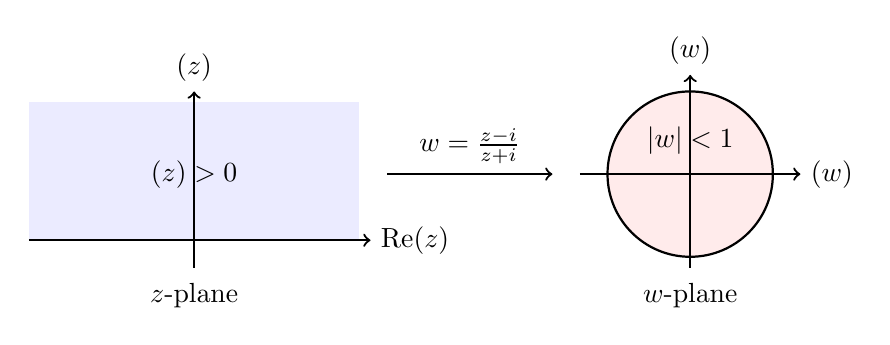
\begin{tikzpicture}[scale=0.7]
	
	% --- LEFT: upper half-plane in z-plane ---
	% Shaded region
	\fill[blue!20, opacity=0.4]
	(-3,0) rectangle (3,2.5);
	
	% Real axis
	\draw[thick, ->] (-3,0) -- (3.2,0) node[right] {$\mathrm{Re}(z)$};
	
	% Imaginary axis
	\draw[thick, ->] (0,-0.5) -- (0,2.7) node[above] {$\imag(z)$};
	
	% Boundary label
%	\node[left] at (-3,0) {$\imag(z)=0$};
	
	% Region label
	\node at (0,1.2) {$\imag(z)>0$};

	% z plane
\node at (0,-1) {$z$-plane};

	
	% --- Arrow for mapping ---
	\draw[->, thick] (3.5,1.2) -- (6.5,1.2) node[midway, above] {$w=\frac{z-i}{z+i}$};
	
	% --- RIGHT: unit disc in w-plane ---
	% Shaded disc
	\fill[red!20, opacity=0.4] (9,1.2) circle (1.5);
	
	% Unit circle boundary
	\draw[thick] (9,1.2) circle (1.5);
	
	% Real axis
	\draw[thick, ->] (7,1.2) -- (11,1.2) node[right] {$\real(w)$};
	
	% Imaginary axis
	\draw[thick, ->] (9, -0.5) -- (9, 3) node[above] {$\imag(w)$};
	
	% Region label
	\node at (9,1.8) {$|w|<1$};
	% 2 plane
\node at (9,-1) {$w$-plane};

	
\end{tikzpicture}
	\end{center}
	\caption{Mapping property of linear fractional transformation $f(z) = (z-i)/(z+i)$.}
\label{fig:exp_map1}	
\end{figure}




\begin{example}
	The complex exponential function $f(z)=e^z$ maps the horizontal strip $\{z:\, -\pi / 2 < \imag(z) < \pi/ 2\}$ conformally and bijectively to the right half plane $\{z:\, \real(z) > 0\}$. 
 (See Fig.~\ref{fig:exp_map1}). 
\end{example}

\begin{figure}
\begin{center}
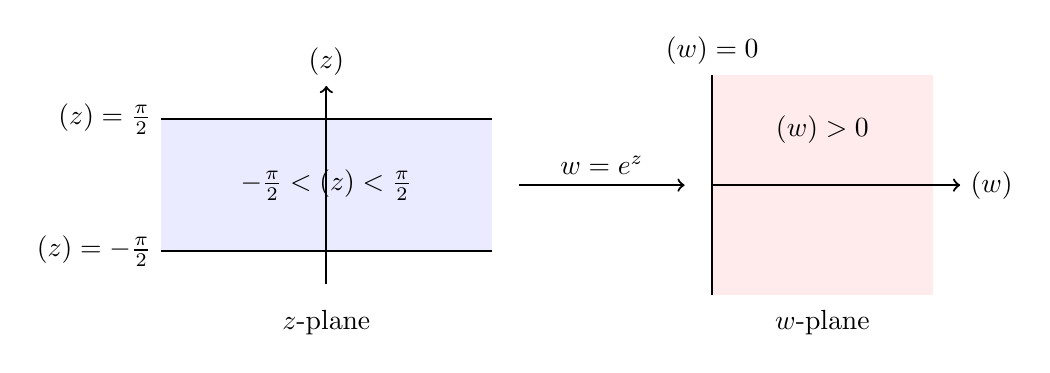
\begin{tikzpicture}[scale=0.7]
	
	% --- LEFT: horizontal strip in z-plane ---
	% Shaded strip
	\fill[blue!20, opacity=0.4]
	(-3,-1.2) rectangle (3,1.2);
	
	% Boundary lines
	\draw[thick] (-3,1.2) -- (3,1.2);
	\draw[thick] (-3,-1.2) -- (3,-1.2);
	
	% Imaginary axis
	\draw[thick, ->] (0,-1.8) -- (0,1.8) node[above] {$\imag(z)$};
	
	% Labels for boundaries
	\node[left] at (-3,1.2) {$\imag(z)=\frac{\pi}{2}$};
	\node[left] at (-3,-1.2) {$\imag(z)=-\frac{\pi}{2}$};
	
	% Label for region
	\node at (0,0) {$-\frac{\pi}{2} < \imag(z) < \frac{\pi}{2}$};
	
	% --- Arrow for mapping ---
	\draw[->, thick] (3.5,0) -- (6.5,0) node[midway, above] {$w=e^z$};
	
	% --- RIGHT: right half-plane in w-plane ---
	% Shaded right half-plane
	\fill[red!20, opacity=0.4]
	(7,-2) rectangle (11,2);
	
	% Boundary line (imaginary axis)
	\draw[thick] (7,-2) -- (7,2) node[above] {$\real(w)=0$};
	
	% Real axis
	\draw[thick, ->] (7,0) -- (11.5,0) node[right] {$\real(w)$};
	
	% Label for region
	\node at (9,1) {$\real(w)>0$};
	
	% w plane
\node at (9,-2.5) {$w$-plane};

	% z plane
\node at (0,-2.5) {$z$-plane};


\end{tikzpicture}
\end{center} 
	\caption{Mapping property of the complex exponential function.}
\label{fig:exp_map2}
\end{figure}


By the chain rule, composition of two conformal maps is also conformal. 

\begin{example}
We can map the right half-plane to the unit disk through the linear fractional transformation in Example~\ref{ex:LFT_conformal}. We can first map the right half-plane to the upper half-plane  by multiplication by~$i$, then apply the function $f(z) = \frac{z-i}{z+i}$. The overall transformation is
$$
f(iz) = \frac{(iz) - i}{(iz) + i} = \frac{z-1}{z+1}.
$$
\end{example}

\begin{example}
We can find a conformal mapping that transform the horizontal strip $S = \{z:\, 0< \imag(z) < \pi\}$ to the unit disk as follows. First, we use the exponential function $z\mapsto \exp(z)$ map $S$ to the upper half-plane.  The apply the transformation $f(z)$ in Example~\ref{ex:LFT_conformal} to map it to the unit disk. The composed transformation is
$$
z \mapsto \frac{e^z -  i}{e^z+i}.
$$
\end{example}




\section{Harmonic functions}

Another necessary condition for being holomorphic is that the real and imaginary parts are both harmonic functions. A twice-differentiable real-valued function $F(x,y)$ is said to be harmonic if it satisfies the Laplace equation
$$
F_{xx} +F_{yy} = 0,
$$
where $F_{xx}$ and $F_{yy}$ are the second partial derivatives of $F$ with respect to $x$ and $y$, respectively.

Suppose that $u(x,y)$ and $v(x,y)$ are twice differentiable, and the second-order derivatives are continuous functions, so that $u_{xy} = u_{yx}$ and $v_{xy} = v_{yx}$. Under these assumptions, we can deduce that the real and imaginary part of a holomorphic function are both harmonic functions. (We will show in a later lecture that the additional smoothness requirements always hold.) In general, we say that a function is in $C^2$ if the  second partial derivatives exist and are continuous.

\begin{svgraybox}
	\begin{theorem}
		Let $f(z)$ be a holomorphic function on a region $R$. If the real part $u(x,y)$ and imaginary part $v(x,y)$ are in $C^2$. Then
		$$
		u_{xx} + u_{yy} = 0 = v_{xx} + v_{yy}
		$$
		in the region $R$.
	\end{theorem}
\end{svgraybox}


\begin{proof}
	The complex function $f(z)$ is holomorphic by assumption, hence must satisfy the Cauchy-Riemann equations $u_x=v_y$ and $u_y = -v_x$. Take partial derivatives with respect to $x$ and $y$,  we obtain $u_{xx}=v_{yx}$ and $u_{yy} = - v_{xy}$. Because we can exchange the order of the partial derivatives, we get
	$$
	u_{xx}+u_{yy}  = v_{yx}-v_{xy} = v_{xy} - v_{xy} = 0.
	$$
	
	Similarly, we can show that $v(x,y)$ is harmonic by first deriving $u_{xy} = v_{yy}$ and $u_{yx} = -v_{xx} $ from the Cauchy-Riemann equations. Then,-
	$$
	v_{xx}+v_{yy}  = -u_{yx}+u_{xy} = -u_{xy} + u_{xy} = 0.
	$$
\end{proof}

In the followings, we will assume that $u(x,y)$ and $v(x,y)$ are $C^2$ functions. We define the notion of harmonic conjugates

\begin{svgraybox}
	\begin{definition} \index{Harmonic conjugate}
		Given a harmonic function $u(x,y)$, we say that $v(x,y)$ is a \df{harmonic conjugate} of $u(x,y)$ if $u(x,y) + iv(x,y)$ is holomorphic in a domain.
	\end{definition}
\end{svgraybox}

Equivalently, we can define that $v(x,y)$ is a harmonic conjugate to $u$ if $u$ and $v$ satisfy the Cauchy-Riemann equations. It is obvious that  harmonic conjugate to a given harmonic functions, if exists, is not unique. It is because, if $v(x,y)$ is a harmonic conjugate to $u(x,y)$, then for any complex constant $C$, the function $v(x,y)+C$ is also a harmonic conjugate.

The existence of harmonic conjugate depends on the topology of the domain on which the function $u(x,y)$ is defined. It is known that if the domain $D$ is simply connected, then a harmonic function $u(x,y)$ defined on $D$ has a harmonic conjugate. We can formulate the problem in terms of differential form. We want to find  a function $v(x,y)$ whose differential is given by
$$
dv = v_xdx + v_y dy = -u_y dx + u_x dy.
$$
Since $u_y$ and $u_x$ are given, the problem of finding a harmonic conjugate to $u(x,y)$ reduces to solving the differential equation above. We prove in the appendix of this section that solution always exists if the region of definition $D$ is simply connected (The proof relies an application of the Green's theorem).

\begin{example}
	We consider the function $$u(x,y) = \sin(x) \cosh(y).$$ This is harmonic because 
	$$
	u_{xx} = - \sin(x) \cosh(y), \ \ \text{ and } \ u_{yy} = \sin (x) \cosh(y).
	$$		
	From the condition $v_x= -u_y = -\sin(x) \sinh(y)$, we can obtain
	$$
	v(x,y) = \int -\sin(x) \sinh(y) \, dx = \cos(x) \sinh(y) + C(y),
	$$
	where $C(y)$ is a function of $y$. By applying the other Cauchy-Riemann equation $v_y =  u_x$, we get
	$$
	v_y = \cos(x)\cosh(y) + C'(y) = u_x = \cos(x)\cosh(y).
	$$
	Hence the function $C(y)$ should be a constant. The harmonic conjugate of $u(x,y)$ can be written as
	$$
	v(x,y) = \cos(x) \sinh(y) + C
	$$
	for some constant $C$. The complex holomorphic function is
	\begin{align*}
		\sin(x) \cosh(y) + i \cos(x) \sinh(y) &= 
		\frac{e^{ix} - e^{-ix}}{2i} \cdot  \frac{e^{y} + e^{-y}}{2} + i 
		\Big(\frac{e^{ix} + e^{-ix}}{2} \cdot \frac{e^{y} - e^{-y}}{2} \Big) \\
		&= \frac{1}{4i}[(e^{ix}- e^{-ix})(e^y + e^{-y}) - (e^{ix}+ e^{-ix})(e^y - e^{-y})] \\
		&= \frac{e^{i(x+iy)} - e^{-i(x+iy)}}{2i} \\
		&= \sin(z).
	\end{align*}
\end{example}


\begin{example}    \label{ex:harmonic_function}
	Find a harmonic conjugate of the function
	$$
	u(x,y) = -2x^2 + x^3+2y^2-3xy^2.
	$$
	
	The function $u(x,y)$ is defined on the whole complex plane. We check that it is harmonic:
	\begin{align*}
		u_x &= -4x + 3x^2-3y^2 \\
		u_{xx}&= -4 + 6x \\
		u_y &= 4y - 6xy \\
		u_{yy} &= 4-6x.
	\end{align*}
	Hence $u_{xx}+u_{yy}$ is identically equal to zero. 
	
	We now proceed to find a harmonic conjugate. We first integrate
	$$
	v_x = -u_y = -4y + 6xy
	$$
	with respect to $x$ and get
	$$
	v(x,y) = \int -4y + 6xy\, dx = -4xy + 3x^2 y  + C(y),
	$$
	where $C(y)$ is a constant that may involve $y$. Differentiate the above with respect to $y$,
	$$
	v_y = -4x+3x^2+C'(y).
	$$
	After comparing with $u_x$, we see that $C'(y) = -3y^2$, and hence $C(y) = -y^3 + C$ for some constant $C$. The answer is
	$$
	v(x,y) = -4xy + 3x^2 y -y^3 + C,
	$$
	where $C$ is any constant.	
\end{example}

%	Using the method of path integral, we can obtain the function $v$ by
%	$$
%	v(a,b) := \int_{(0,0)}^{(a,b)} (6xy-4y)dx + (-4x+3x^2-3y^2)dy .
%	$$
%	for any $(a,b) \in \mathbb{R}^2$. For the ease of calculations, we picked the origin $(0,0)$ as the start point of the path, and take the direct path from $(0,0)$ to $(a,b)$. Parametrize this path by
%	$$
%	\begin{cases}
	%		x = ta \\
	%		y = tb
	%	\end{cases}
%	$$
%	for $0\leq t \leq 1$. We evaluate the path integral
%	\begin{align*}
	%		v(a,b) &= \int_0^1 (6t^2 ab-4tb)a +
	%		(-4ta+3t^2 a^2-3t^2b^2)b\, dt \\
	%		&= \int_0^1 -8abt + (9a^2b -3b^3)t^2\, dt\\
	%		&= - 4ab + 3a^2b  - b^3 +C
	%	\end{align*}
%	where $C$ is a constant.
%	Hence, the function $v(x,y) = -4xy + 3x^2y - y^3 +C$ is a harmonic conjugate of $u(x,y)$.
%	
%	The complex function $u(x,y)+i v(x,y)$ is indeed a function of $z$,
%	$$
%	-2x^2 + x^3+2y^2-3xy^2+ i ( -4xy + 3x^2y - y^3) = (x+iy)^3-2(x+iy)^2 = z^3-2z^2.
%	$$
%\end{example}
%
%
When $u(x,y)$ is a {\em polynomial} in $x$ and $y$, there is a slick method to directly obtain the complex function $f(z)$ whose real part is $u(x,y)$. 
%If $u(x,y)$ is a harmonic polynomial, then by the line integral method, we know that it is the real part of a holomorphic function $f$. The function $f$ should be a polynomial in $x$ and $y$, because we are integrating polynomials in $x$ and $y$ in the line integral method. Potentially, this could be a function $f(z,\bar{z})$ of $z$ and $\bar{z}$, but since $\bar{\del} f(z,\bar{z})=0$, the function $f(z,\bar{z})$ can only depend on $z$.
We can write $z=x+iy$ and exploit the following equalities 
$$
u\big(\frac{z+\bar{z}}{2}, \frac{z-\bar{z}}{2i}\big) = u(x,y) = \real(f(z)) = \frac{f(z) + \overline{f(z)}}{2} = \frac{f(z) + f(\bar{z})}{2}.
$$
In the last step we can replace $\overline{f(z)}$ by $f(\bar{z})$, because $f$ is a polynomial in $z$.

We can re-do Example~\ref{ex:harmonic_function} by using this method.
\begin{align*}
	u\big(\frac{z+\bar{z}}{2}, \frac{z-\bar{z}}{2i}\big) &=
	-2 \big( \frac{z+\bar{z}}{2} \big)^2 + \big( \frac{z+\bar{z}}{2} \big)^3 +2 \big( \frac{z-\bar{z}}{2i} \big)^2 - 3 \big( \frac{z+\bar{z}}{2} \big) \big( \frac{z-\bar{z}}{2i} \big)^2 \\
	&= -z^2 - \bar{z}^2 + z^3/2 + \bar{z}^3/2.
\end{align*}
By comparing it with $(f(z)+f(\bar{z}))/2$, we obtain $f(z) = -2z^2 + z^3$.

One can further streamline this method by directly computing
\begin{equation}
	\phantom{=}	2u\big( \frac{z}{2}, \frac{z}{2i}\big) - u(0,0).
	\label{eq:harmonic_to_holomorphic}
\end{equation}
(We subtract $u(0,0)$ in order to preserve the constant term.)
This will be a complex differentiable function $f$ in variable $z$ only and the real part is precisely $u(x,y)$. The complex function in Example~\ref{ex:harmonic_function} is thus.
\begin{align*} &2u\big( \frac{z}{2}, \frac{z}{2i}\big) - u(0,0)\\
	&= 
	2\big(-2(\frac{z}{2})^2 + (\frac{z}{2})^3 + 2(\frac{z}{2i})^2 - 3(\frac{z}{2}) (\frac{z}{2i})^2\big) \\
	&= -2z^2+z^3.
\end{align*}



\section{Application: Smith Chart as a conformal M\"obius transformation}

\index{Smith chart}
Among the simplest examples of a M\"obius transformation with interesting
geometric behavior is the map
\[
\Phi(z)=\frac{z-1}{\,z+1\,}.
\]
Although this transformation appears in electrical engineering under the
name ``reflection coefficient,'' its structure is entirely classical.
From the point of view of complex analysis, the so-called \emph{Smith
	chart} is nothing more than the image of the right half-plane under the M\"obius transformation~$\Phi$. (See Fig.~\ref{fig:Smith_chart})

\begin{figure}
	\begin{center}
\includegraphics*[width=7cm]{Bare_Bones_Smith_Chart_-_with_annotations.png}
	\end{center}
	\caption{Smith chart (from wikipedia)}.
	\label{fig:Smith_chart}
\end{figure}

{\em Mapping the right half--plane to the unit disk}.
Let
\[
H=\{z\in\mathbb{C} : \real(z) > 0\}
\]
denote the right half--plane. A direct computation shows that
\[
|\Phi(z)| < 1
\quad\Longleftrightarrow\quad
|z-1| < |z+1|
\quad\Longleftrightarrow\quad
\real(z) > 0.
\]
Thus $\Phi$ maps $H$ conformally onto the open unit disk
\[
D(0,1) =\{w\in\mathbb{C} : |w|<1\}.
\]
The boundary line $\real(z)=0$ is mapped to the unit circle $|w|=1$, and
Möbius transformations send generalized circles (circles or lines) to
generalized circles. Consequently, the coordinate lines in $H$ become
families of circles inside the unit disk.

{\em Geometry of the image}. 
Write $z=x+iy$ with $x>0$. Then:

\begin{itemize}
	\item \textbf{Vertical lines $x=\text{constant}$} map to circles in
	the unit disk whose centers lie on the real axis. Each such circle is orthogonal to the unit circle.
	
	\item \textbf{Horizontal lines $y=\text{constant}$} map to circles
	tangent to the unit circle at the point $w=1$. Their centers lie on
	the real axis to the right of the disk.
\end{itemize}

Thus the familiar grid of the Smith chart is simply the image of the
rectangular coordinate system on $H$ under the Möbius transformation
$\Phi$.



\section{Additional proof for existence of harmonic conjugate}
\label{sec:harmonic_conjugate}
In this optional section we prove that harmonic conjugate of a harmonic function exists if the domain of definition is simply connected.   We assume that the function of interest is continuously differentiable.  In the followings, the functions $u$ and $v$ must be sufficiently smooth so that the Green's theorem can be applied.



\begin{svgraybox}
	\begin{theorem}
If the domain of definition is simply connected, then 
harmonic function has a harmonic conjugate in the same domain.
	\end{theorem}
\end{svgraybox}

\begin{proof}

Consider the differential form
$$
dv = v_xdx + v_y dy =-u_y dx + u_x dy. 
$$
We claim that the line integral 
\begin{equation}
	\int_{(x_0,y_0)}^{(x_1,y_1)} -u_y dx + u_x dy
	\label{eq:harmonic_conjugate_proof}
\end{equation}
does not depend on path. We can see it from Green's theorem, using the assumption that $D$ is simply connected and $u(x,y)$ satisfies the Laplace equation. If $C$ is a closed path enclosing a region $S$, we have
$$
\oint_C -u_y dx + u_x dy = \iint_S \frac{\partial}{\partial x} u_x - \frac{\partial}{\partial y}(-u_y) \, ds = \iint_S u_{xx}+u_{yy} \, ds= 0.
$$

We can thus define a function $v(x,y)$ by first fixing a point $(x_0,y_0)$ in the domain $D$ of $u(x,y)$, and define a function $v(x,y)$ by
\begin{equation}
	v(x,y) \triangleq \int_{(x_0,y_0)}^{(x,y)}-u_y dx + u_x dy
	\label{eq:u_harmonic_conjugate}
\end{equation}
for any point $(x,y)$ in $D$. This is well-defined because the line integral is independent of path, and there is at least one path connecting $(x_0,y_0)$ and $(x,y)$.

We now check that the function $v(x,y)$ so defined is a harmonic conjugate of $u(x,y)$. Let $(a,b)$ be any point in $D$. The partial derivative of $v$ with respect to $x$ at this point is
\begin{align*}
	v_x(a,b) &= \lim_{\Delta x\rightarrow 0} 
	\frac{v(a+\Delta x,b)-v(a,b)}{\Delta x} \\
	&= \lim_{\Delta x\rightarrow 0} \frac{1}{\Delta x} \int_{(a,b)}^{(a+\Delta x,b)}  -u_y dx + u_x dy \\
	&= \lim_{\Delta x\rightarrow 0} \frac{1}{\Delta x} \int_{(a,b)}^{(a+\Delta x,b)}  -u_y dx\\
	&= - u_y(a,b).
\end{align*}
In the last step we have used the assumption that $u_y$ is continuous at $(a,b)$.

Likewise, by consider the partial derivative of $v$ with respect to $y$, we get
\begin{align*}
	v_y(a,b) &= \lim_{\Delta y\rightarrow 0} 
	\frac{v(a,b+\Delta y)-v(a,b)}{\Delta y} \\
	&= \lim_{\Delta y\rightarrow 0} \frac{1}{\Delta y} \int_{(a,b)}^{(a,b+\Delta y)}  -u_y dx + u_x dy \\
	&= \lim_{\Delta y\rightarrow 0} \frac{1}{\Delta y} \int_{(a,b)}^{(a,b+\Delta y)}  u_x dy\\
	&= u_x(a,b).
\end{align*}
We have used the continuity of $u_x$ in the last step. This proves that the Cauchy-Riemann equations are satisfied at the point $(a,b)$. By the sufficient condition in Theorem~\ref{thm:complex_differentiable}, we conclude that $u(x,y)+i v(x,y)$ is a holomorphic function in the domain~$D$.


We can now conclude that a harmonic conjugate of $u(x,y)$ can be written as in \eqref{eq:u_harmonic_conjugate} when $D$ is simply connected. 
\end{proof}


This theorem provides the existence proof of harmonic conjugate. If can find a function $v(x,y)$ in closed-form expression such that $dv = -u_y dx + u_x dy$, then this function is a harmonic conjugate of $u(x,y)$. In general, the integration in \eqref{eq:harmonic_conjugate_proof} is not tractable. The purpose of the proof is to give a sufficient condition under which harmonic conjugate exists. 








\section*{Summary}

\begin{itemize}
	\item (Holomorphicity) A complex function $f(z)$ is holomorphic at a point $z_0$ if it is complex differentiable at all points in a neighborhood of~$z_0$. If $f(z)$ is complex differentiable at all points in a domain $D$, then $f(z)$ is holomorphic in~$D$. An entire function is a complex function that is holomorphic in the whole complex plane.





	
	\item (Differential rules) The differential rules from calculus, such as the product rule, quotient rule, and the chain rule, also apply for holomorphic functions.
	
	
\item (Holomorphic at $\infty$) We study the behavior of a complex function $f(z)$ at the point at infinity by making a change of variable $w=1/z$. By defining $g(w)=f(1/w)$, we say that $f(z)$ is continuous (resp. differentiable, holomorphic) at $\infty$ if $g(w)$ is continuous (resp. differetiable, holomorphic) at $w=0$.

\item (Smooth curve) A parametric curve in $\mathbb{C}$ is a continuous function $\gamma: [a,b]\rightarrow \mathbb{C}$. We say that this is a smooth (resp. piece-wise smooth) curve if $\gamma$ is a continuously differentiable (resp. piece-wise continuously differentiable). 

\item (Conformal mapping) The transformation induced by a complex function is conformal if it complex differentiable and the complex derivative is nonzero.	
	
\item (Laplace equation) 	The real and imaginary parts of a holomorphic function satisfy the Laplace equation, if they are twice differentiable.

	\item (Harmonic conjugate)  A harmonic function $v(x,y)$ is called a harmonic conjugate of harmonic conjugate $u(x,y)$ if $u(x,y)+iv(x,y)$ is harmonic.
	
%	\item (Dirichlet's problem) We can use conformal mapping to transform a Dirichlet problem on a simply connected domain to a Dirichlet problem on the unit circle.
	
	\item (Existence of harmonic conjugate) 
	Given a harmonic function defined on a simple connected domain, harmonic conjugate exists in the same domain.
\end{itemize}

\section*{Exercise}

\renewcommand{\labelenumi}{\arabic{enumi}.}
\begin{enumerate}
	
\item Let $f$ denote a holomorphic function in a domain. Prove 
\begin{enumerate}
\item $f$ is a constant function if $\real(z)$ is a constant function \item $f$ is a constant function if $\imag(z)$ is a constant function.
\item $f$ is a constant function if $|z|$ is a constant function. \end{enumerate}

	\item Expand the function in the form of power series $\sum_{k=0}^\infty a_k z^k$.
\begin{flalign*}
	(a)\ & \frac{1+z}{1+iz} & 
	(b)\ & \frac{1}{(1+z)(i+z)} &
	(c)\ & \frac{1}{1+z^3} &&&&&
\end{flalign*}

\item By repeated differentiating the function $1/(z+1)^2$, write down the power series expansion of $1/(z+1)^2$.

\item Prove that the radius of convergence $R$ of a series $\sum_{k=0}^\infty a_k z^k$ can be expressed as
$$
R = \sup \{ |z| :\, \lim_{k\rightarrow\infty} a_kz^k =0 \}.
$$

\item (Abel limit theorem) Let $a_n$, for $n\geq 0$ be complex numbers such that $\sum_{n=0}^\infty a_n$ converges. Define the power series
$$
f(z) = \sum_{n=0}^\infty a_n z^n.
$$
Show that if $z\rightarrow1 $ in such a way that $z$ stays inside the disk $|z-0.5|\leq 0.5$, then $f(z)\rightarrow f(1)$.

(Hint: A complex number $z$ is inside the disk $|z-0.5|\leq 0.5$ if and only if $|1-z| + |z| \leq 1$. By re-defining $a_0$, we can assume without loss of generality that $\sum_{n} a_n = 0$. For $n\geq 1$, consider the polynomial $s_n(z) = a_0+a_1z+\cdots a_nz^n$, and the partial sum $s_n \triangleq s_n(1) = a_0+\cdots + a_n$. Prove that
$$
s_n(z) = (1-z) (s_0 + s_1z + \cdots + s_{n-1}z^{n-1} ) + s_n z^n,
$$
and show that both terms approaches zero.
)


\item Consider the power series $\sum_{n=1}^\infty \frac{z^n}{n}$.

\begin{enumerate}
	\item Show that when $z=1$, this series diverges.
	
	%When $z=1$, the power series $\sum_{n=1}^\infty 1/n$ is the harmonic series and is divergent.
	
	\item 
	Let $z\neq 1$ be any other point on the unit circle. We first prove the following identity for each integer $m$,
	\begin{equation}
		\sum_{n=1}^m \frac{z^n}{n} = \frac{z}{1-z} \Big( \sum_{n=1}^{m-1} \frac{1}{n(n+1)} - \sum_{n=1}^{m-1}  \frac{z^n}{n(n+1)} \Big) + \frac{z(1-z^m)}{m(1-z)}.
		\label{eq:1}
	\end{equation}
	%The first term
	%$$\frac{z}{1-z} \Big( \sum_{n=1}^{m-1} \frac{1}{n(n+1)} - \sum_{n=1}^{m-1}  \frac{z^n}{n(n+1)} \Big) 
	%$$
	%on the right-hand side of \eqref{eq:1} can be expanded as the sum of the following sums
	%\begin{align*}
	%	\frac{1}{1\cdot 2} &(z)\\
	%	\frac{1}{2\cdot 3} &(z+z^2)\\
	%	%	\frac{1}{3\cdot 4} &(z+z^2+z^3)\\
	%	%	\frac{1}{4\cdot 5} &(z+z^2+z^3+z^4)\\
	%	& \vdots \\
	%	\frac{1}{(m-1)m} &(z+z^2+z^3+z^4+ \cdots + z^m)
	%\end{align*}
	%If we add the terms ``vertically'' by grouping terms with the same degree, and use the telescoping sum
	%$$
	%\frac{1}{n(n+1)}+\frac{1}{(n+1)(n+2)}+\cdots + \frac{1}{(m-1)m} = \frac{1}{n}-\frac{1}{m},
	%$$
	%we get
	%$$
	%\frac{z}{1-z} \Big( \sum_{n=1}^{m-1} \frac{1}{n(n+1)} - \sum_{n=1}^{m-1}  \frac{z^n}{n(n+1)} \Big)
	%=\sum_{n=1}^m \frac{z^n}{n} - \frac{1}{m}\sum_{n=1}^m z^n.
	%$$
	%From this we can obtain \eqref{eq:1} by noting that $\sum_{n=1}^m z^n = \frac{z(1-z^m)}{1-z}$.
	
	Using the identity in \eqref{eq:1}, we can prove that the power series $\sum_n z^n/n$ converges for $z\neq 1$ on the unit circle by comparing with the convergent power series 
	$$
	\sum_{n=1}^\infty \frac{1}{n(n+1)}.
	$$
	Use the fact that
	$$
	\sum_{n=1}^\infty \frac{z^n}{n(n+1)}
	$$
	converges absolutely for all $z$ with $|z|=1$, and the last term $ \frac{z(1-z^m)}{m(1-z)}$ in \eqref{eq:1}
	converges to zero as $m$ tends to infinity.
\end{enumerate}




\item Let $f(z)$ be a polynomial in complex variable $z$. Prove that $\overline{f(\bar{z})}$ is complex differentiable for all $z\in\mathbb{C}$.

\item (L'Hospital rule for $0/0$)

\begin{enumerate}
	\item Let $z_0$ be a finite complex number
 Suppose $f(z)$ and $g(z)$ are complex differentiable at $z_0$, $f(z_0)=g(z_0)=0$, and $g'(z_0)\neq 0$. Prove that
$$
\lim_{z\rightarrow z_0}  \frac{f(z)}{g(z)} = \frac{f'(z_0)}{g'(z_0)}.
$$ 
\item L'Hospital rule continues to hold at the point at infinity in the following sense. Suppose $f(z)$ (resp. $g(z)$) behaves like $a/z$ (resp. $b/z$) for some constant $a$ (resp. $b$) when $z$ tends to infinity. Further, suppose that $b\neq 0$. Then
$$
\lim_{z\rightarrow \infty}  \frac{f(z)}{g(z)} = \frac{a}{b}.
$$ 

(The mathematical meaning of $f(z)$ behaves like $a/z$ is $\lim_{z\rightarrow\infty} z f(z) = a$.)
\end{enumerate}

\item Suppose $f'(z)$ for $|z|>R$ for some real number $R$ and $\lim_{z\rightarrow \infty} f(z)$ exists. Show that if $f(z)$ is differentiable at the point at infinity, then the derivative is given by
	$$
	f'(\infty) = \lim_{z\rightarrow \infty} z^2 f'(z).
	$$


\item Consider the function
$$
u(x,y) = \sinh(x) \cos(y).
$$

\begin{enumerate}

\item Show that $u(x,y)$ is a harmonic function.

\item Find the harmonic conjugate of $u(x,y)$.

\item  Let $v(x,y)$ be your answer in part (b). Write the holomorphic function $u(x,y) + iv(x,y)$ as a function of $z$. 
\end{enumerate}



\item In general, the Mean Value Theorem does not hold for function in complex variable. Consider the function $f(z)=z^3$, which is complex differentiable everywhere, and the line segment between 1 and $i$. Represent a point on this segment by $x+(1-x)i$, for $x\in[0,1]$.  Show that 
$$f'(x+(1-x)i) \neq \frac{f(i)-f(1)}{i-1}$$ 
for all $x\in[0,1]$.

\item Solve the system
$$
u_x = v_y, \ \ u_y = -v_x
$$
under the assumption that $u(x,y) = x^2-y^2+g(y)$, where $g(y)$ is a function of~$y$. Find all possible holomorphic functions $f$ whose real part is equal to~$u$.

\item Suppose $f(z)$ is holomorphic in some region $D$. Prove that
$$
\frac{\partial}{\partial z} \frac{\partial}{\partial \bar{z} } |f(z)|^2
= |f'(z)|^2
$$
for $z\in D$. (Use the property that $\frac{\partial }{\partial \bar{z}} \overline{f(z)} =
\overline{\frac{\partial f}{\partial z}(z) }$.)

\item Find a holomorphic function $f(z)=u(x,y)+iv(x,y)$ such that
$u(x,y)^2 + i v(x,y)^2$ is also holomorphic.

\item Let $f(x)$ be a real function defined by
$$
f(x) \triangleq \begin{cases}
	0 & \text{ if } x\leq 0 \\
	e^{-1/x} & \text{ if } x >0.
\end{cases}
$$
Show that $f(x)$ is infinitely differentiable at all points, but we cannot represent $f(x)$ using power series at $x=0$.


\item The Joukowsky map is defined by
$$
J(z) \triangleq \frac{1}{2}\big(z + \frac{1}{z} \big)
$$
for $z \in \mathbb{C} \setminus\{0\}$.
We may extend the domain to the extended complex plane by continuity by setting
$$
J(0) \triangleq \infty, \ J(\infty) \triangleq \infty.
$$
With this convention, the Joukowsky function has the special property that 
$$
J(z) = J(1/z) 
$$
for all $z\in \bar{\mathbb{C}}$.

\begin{enumerate}
\item Show that the derivative of $J(z)$ is equal to
$$
J'(z) = \frac{1}{2}\big( 1 - \frac{1}{z^2}\big) = \frac{1}{2} \frac{(z-1)(z+1)}{z^2},
$$
for $z\neq 0$. 

\item Compute the derivative of $1/J(z)$ at $z=0$, and show that
$$
\frac{d}{dz} \frac{2z}{z^2+1} \Big|_{z=0}= 2.
$$
Moreover, show that $\big(1/J(z)\big)'$ approaches 0 as $z$ approaches the point at infinity.
Hence, $J(z)$ is conformal in the extended complex plane except~$\pm 1$.
\end{enumerate}


\end{enumerate}





